% ========================================= TEMPLATE INFO ========================================
%
% Author:       P4ntomime
% Version:      1.0.0
% Last updated: 2024-02-18
% Brief:        A LaTeX template for summaries. See README.md for more information.
% 
% ================================================================================================
\documentclass[8pt, a4paper, twoside]{extarticle}
% Font size:    8pt
% Paper size:   A4
% style:        twoside (needed, so odd and even pages have different margins)
% orientation:  portrait. (use 'landscape' for landscape orientation)


% ========================================= DOCUMENT INFO =========================================
\def\title{Regelungstechnik 4}                              % title
\def\shorttitle{RegT4}                                      % short title (displayed as PDF title)
\def\dozent{Prof. Dr. Markus Kottmann}                      % lecturer
\def\semester{FS 2025}                                      % semester
\def\author{Simone Stitz, Gian Marco Näf}                                   % author(s)
\def\repo{https://github.com/Giamo08/Zusammenfassungen}     % repository link
\def\version{1.0.\today}                                    % version
\def\pagelimit{20}                                          % page limit -> causes pages after limit to be red
\def\titleoption{compact}                                   % options: ultra compact, compact, normal
\def\enableToC{true}

% ================================= PACKAGES, SETUP AND COMMANDS ==================================
\input{preamble.tex}


% =========================================== DOCUMENT ============================================
\begin{document}
    \begin{layout}
        \part{Regelungstechnik 4}
        \section{Zustandsraumdarstellung (ZRD)}

\subsection{Zustrandsraumdarstellung von MIMO-Systemen}{153-154}

Der Vorteil der Zustandsraumdarstellung gegenüber der I/O-Beschreibung liegt darin, dass die internen Signale des Systems
(Zustandsvariablen) mitmodelliert werden. \\
Die ZRD kann aus dem Blockdiagramm abgeleitet werden. Umgekehrt kann aus der ZRD das Blockdiagramm
gezeichnet werden.

\smallskip

Die ZRD von MIMO-Systemen wird folgendermassen beschrieben:


\begin{center}
    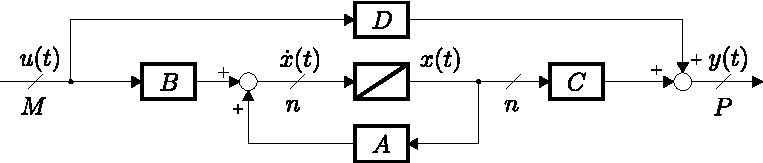
\includegraphics[width=0.75\columnwidth]{images/ZRD_blockdiagramm.pdf}
\end{center}

\begin{minipage}[c]{0.6\columnwidth}
        \fbox{\parbox{0.95\columnwidth}{
        $$ \dot{x}(t) = \bm{A} \cdot x(t) + \bm{B} \cdot u(t) $$
        $$ y(t) = \bm{C} \cdot x(t) + \bm{D} \cdot u(t) $$
    }}
\end{minipage}
\hfill
\begin{minipage}[c]{0.35\columnwidth}
    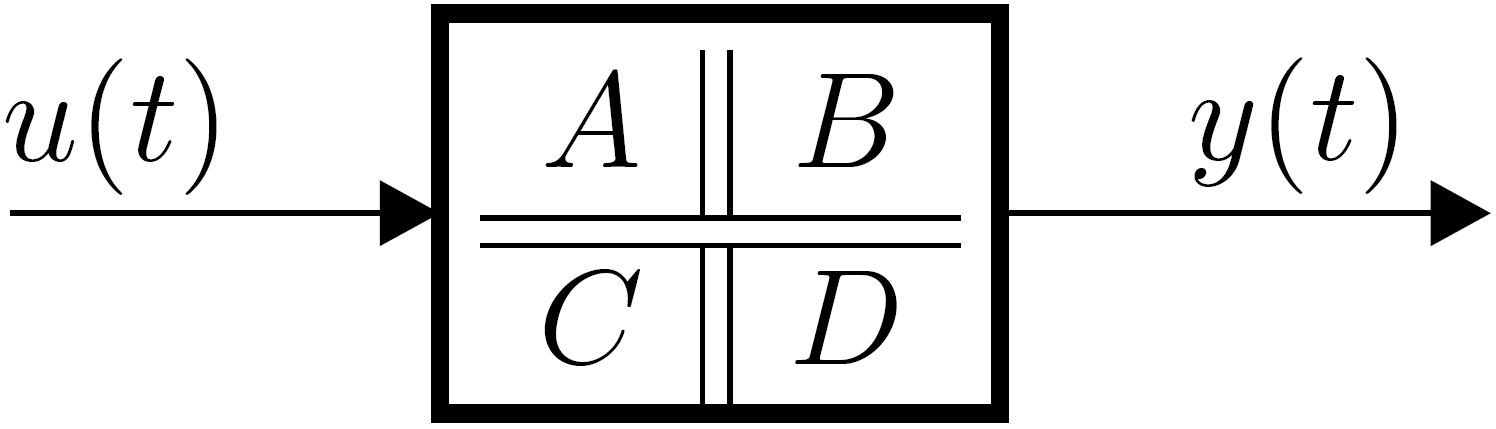
\includegraphics[width=\columnwidth]{images/ZRD_matrix_kompakt.png}
\end{minipage}


\begin{ctabular}{cll}
    \toprule
    $u(t) \in \mathbb{R}^{M}$               & Eingangsvektor    & fasst Eingangsgrössen in Vektor zusammen          \\
    \midrule
    $x(t)\in \mathbb{R}^{n}$                & Zustandsvektor    & fasst Zustände in Vektor zusammen                 \\
    \midrule
    $y(t)\in \mathbb{R}^{P}$                & Ausgangsvektor    & fasst Ausgangsgrössen in Vektor zusammen          \\
    \midrule
    $\bm{A} \in \mathbb{R}^{n \times n}$    & Systemmatrix      & beschreibt (Eigen-)Dynamik des Systems,           \\
                                            &                   & beschreibt \textbf{Stabilität} des Systems        \\
    \midrule
    $\bm{B} \in \mathbb{R}^{n \times M}$    & Eingangsmatrix    & beschreibt, wie der Eingang auf den               \\
                                            &                   & Zustandsvektor einwirken kann                     \\
    \midrule
    $\bm{C} \in \mathbb{R}^{P \times n}$    & Ausgangsmatrix    & beschreibt, welche Zustandsvariablen (oder        \\
                                            &                   & Linearkombinationen davon) \textbf{messbar} sind  \\
    \midrule
    $\bm{D} \in \mathbb{R}^{P \times M}$    & Durchgangsmatrix  & beschreibt direkte Kopplung zwischen Ein- und     \\
                                            &                   & Ausgang                                           \\
    \bottomrule
\end{ctabular}


\textbf{Hinweis:} Für Regelstrecken gilt aufgrund ihres Tiefpassverhaltens meist $\bm{D} = 0$


\subsubsection{ZRD für DGL der Ordnung $\bm{n}$}

\vspace{-0.2cm}

\begin{minipage}[c]{0.58\columnwidth}
    Für eine DGL der Ordnung $n$ werden die Zustände des Zustandsvektors $x$ jeweils so gewählt, dass der erste Zustand der 
    \textbf{unabgeleiteten} Variable entspricht und der letzte Zustand der $n-1$-ten Ableitung. \\
    \textrightarrow\ 'Kette' von Integratoren
\end{minipage}
\hfill
\begin{minipage}[c]{0.4\columnwidth}
    $$ x = \begin{bmatrix} x \\ \dot{x} \\ \vdots \\ x^{(n-1)}\end{bmatrix}
    \quad \Rightarrow\
    \dot{x} = \begin{bmatrix} \dot{x} \\ \ddot{x} \\ \vdots \\ x^{(n)}\end{bmatrix} $$
\end{minipage}


\subsection{Zustrandsraumdarstellung von SISO-Systemen}{154}

\begin{minipage}[c]{0.5\columnwidth}
        \fbox{\parbox{0.95\columnwidth}{
        $$ \dot{x}(t) = \bm{A} \cdot x(t) + b \cdot u(t) $$
        $$ y(t) = c \cdot x(t) + d \cdot u(t) $$
    }}
\end{minipage}
\hfill
\begin{minipage}[c]{0.45\columnwidth}
    Wegen $M = P =1$ werden die Matritzen $\bm{B}$ und $\bm{C}$ zu Vektoren. \\
    $\bm{D}$ wird zu einem Skalar.
\end{minipage}


\subsection{Verfahren mit ZRD -- Übersicht}

Zum Thema ZRD werden die folgenden Verfahren genauer betrachtet, bevor diese auf die Regelungstechnik angewendet werden.

\smallskip

\begin{tabular}{ll}
    \tabitem ZRD aus Modellierung nach physikalischen Prinzipien                & \ref{ZRD via physikalischer Modellbildung}            \\
    \tabitem Lineariserung einer nichtlinearen ZRD                              & \ref{Linearisierung einer ZRD}                        \\
    \tabitem ZRD aus einer UTF oder DGL bestimmen                               & \ref{Zustandsraumdarstellung aus einer UTF oder DGL}  \\
    \tabitem Herauslesen der ZRD aus einem Blockdiagramm                        & \ref{Zustandsraumdarstellung aus Blockdiagramm}       \\
    \tabitem Aggregation von Teilsystem (Serie-, Parallel-, Kreisschaltung)     & \ref{Aggregation von Teilsystemen}                    \\
    \tabitem Ähnlichkeitstransformation durch andere Wahl des Zustandsvektors   & \ref{Ähnlichkeitstransformation}                      \\
\end{tabular}


\subsection{ZRD via physikalischer Modellbildung}
\label{ZRD via physikalischer Modellbildung}

Aus einem physikalischen System werden die Eingang- und Ausgangssignale, sowie die Zustände bestimmt. Diese werden mathematisch / physikalisch
beschrieben und als ZRD dargestellt.

\subsubsection{Vorgehen -- Herleitung eines ZRD-Modells}

\begin{enumerate}
    \item Anzahl Speicher (Integratoren) bestimmen
    \item Wahl der Zustandsgrössen
    \item Beschreibung der \textbf{Änderung} (Ableitungen) der Zustandsgrössen als Gleichungen
    \item Substitution der 'nicht-Zustandsgrössen' mittls algebraischer Gleichungen
    \item Bilden der Zustands- und Ausgangsgleichungen
    \item Darstellung in Matrix-Notation
\end{enumerate}



\example{ZRD eines RLC-Systems}{155-156}

\begin{minipage}[t]{0.3\columnwidth}
    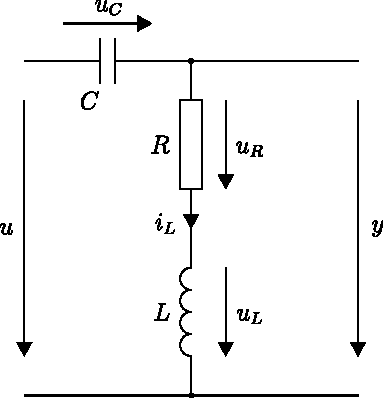
\includegraphics[width=\columnwidth, align=t]{images/ZRD_beispiel_schaltkreis.pdf}
\end{minipage}
\hfill
\begin{minipage}[t]{0.67\columnwidth}
    \begin{outline}
        \1 SISO-System mit zwei Speichern \textrightarrow\ zwei Zustände
            \2 Kondensator \textrightarrow\ $u_C$ (bzw. Ladung)
            \2 Spule \textrightarrow\ $i_L$
    \end{outline}

    \medskip
    
    Somit ergibt sich folgender Zustandsvektor
    $$ x(t)   = \begin{bmatrix} x_1 \\ x_2 \end{bmatrix}
                    = \begin{bmatrix} u_C \\ i_L \end{bmatrix} $$

                
    Die Netzwerkgleichungen ergeben sich aus dem Schema.
\end{minipage}

\smallskip

\renewcommand{\arraystretch}{1.5}
\begin{tabular}{lll}
    Knoten:             & $C \cdot \dot{u}_C = i_C = i_L$                               & \textrightarrow\ $\dot{u}_C = \frac{i_L}{C}$                                          \\
    Eingangsmasche:     & $L \cdot \dot{i}_L = u - u_C - u_R = u - u_C - R \cdot i_L$   & \textrightarrow\ $\dot{i}_L = \frac{u}{L} - \frac{u_C}{L} - \frac{R}{L} \cdot i_L$    \\
    Äussere Masche:     & $u = u_C + y$                                                 & \textrightarrow\ $y = u - u_C$                                                        \\
\end{tabular}
\renewcommand{\arraystretch}{1}

\medskip

Die drei (linearen) Gleichungen rechts können direkt in die ZRD gebracht werden, indem sie in Matritzen geschrieben werden.

\vspace{-0.4cm}

\begin{align*}
    \dot{x}(t)  &= \begin{bmatrix} \dot{u}_C \\ \dot{i}_L \end{bmatrix}
                 = \begin{bmatrix} 0 & \frac{1}{C} \\ - \frac{1}{L} & - \frac{R}{L} \end{bmatrix} \cdot \overbrace{ \begin{bmatrix} u_C \\ i_L \end{bmatrix} }^{x(t)}
                 + \begin{bmatrix} 0 \\ \frac{1}{L} \end{bmatrix} \cdot u(t)\\
    y(t)        &= \begin{bmatrix} -1 & 0 \end{bmatrix} \cdot  \underbrace{ \begin{bmatrix} u_C \\ i_L \end{bmatrix} }_{x(t)} + 1 \cdot u(t)
\end{align*}

\vspace{-0.3cm}

%-----------------------------------------------------------------------------------------------------------------------------------
\example{Feder-Masse-System}

Kraftbilanz:

\[
m\ddot p = F_u-kp
\]

Zustände:

\[
x_1=p,
\qquad
x_2=\dot p
\]

ZRD:

\[
\dot x=
\begin{bmatrix}
0 & 1\\
-\frac{k}{m} & 0
\end{bmatrix}
x+
\begin{bmatrix}
0\\
\frac{1}{m}
\end{bmatrix}
u
\]

\[
y=
\begin{bmatrix}
1 & 0
\end{bmatrix}
x
\]
%------------------------------------------------------------------------------------------------------------------------------------

\subsection{Linearisierung einer ZRD}{168}
\label{Linearisierung einer ZRD}

Die Linearisierung eines Systems erfolgt üblicherweise in einem Arbeitspunkt, damit relativ einfach ein Regler für diesem Arbeitspunkt 
entwickelt werden kann.

\smallskip

Wenn ein System in einem Arbeitspunkt linearisiert wird, has das zur Folge,

\begin{enumerate}
    \item dass das Verhalten des nichtlinearen Systems in einer 'kleineren' Umgebung um den Arbeitspunkt erhalten bleibt.
    \item dass das linearisierte System dieses Verhalten, entsprechend 'gestreckt', im ganzen Zustandsraum zeigt.
\end{enumerate}


\subsubsection{Linearisierte ZRD}

Die linearisierte ZRD für ein nichtlineares System in einem Arbeitspunkt mit $f(x_0, u_0) = 0$ und $y_0 = g(x_0, u_0)$ kann gewonnen werden, indem 
die 'Deltas' gebildet werden. \\
(Die $\Delta$-Symbole werden in der Notation jedoch oft weggelassen.)

\begin{ctabular}{llll}
    Zustandsgleichung(en)   & $\dot{x} = f(x, u)$ & \textrightarrow\  & $\Delta \dot{x} = A \cdot \Delta x + B \cdot \Delta u$    \\
    Ausgangsgleichung(en)   & $y = g(x, u)$       & \textrightarrow\  & $ \Delta y = C \cdot \Delta x + D \cdot \Delta u $
\end{ctabular}

Dazu werden die folgenden Jacobi-Matritzen benötigt, welche im Arbeitspunkt $(x_0, u_0)$ ausgewertet werden.

$$ 
    A =
    \left. \begin{bmatrix}
        \frac{\partial f_1}{\partial x_1} & \cdots & \frac{\partial f_1}{\partial x_n} \\
        \vdots & \ddots & \vdots \\
        \frac{\partial f_n}{\partial x_1} & \cdots & \frac{\partial f_n}{\partial x_n}
    \end{bmatrix} \right|_{x_0, u_0}
    \quad
    B =
    \left. \begin{bmatrix}
        \frac{\partial f_1}{\partial u_1} & \cdots & \frac{\partial f_1}{\partial u_M} \\
        \vdots & \ddots & \vdots \\
        \frac{\partial f_n}{\partial u_1} & \cdots & \frac{\partial f_n}{\partial u_M}
    \end{bmatrix} \right|_{x_0, u_0}
$$

$$
    C =
    \left. \begin{bmatrix}
        \frac{\partial g_1}{\partial x_1} & \cdots & \frac{\partial g_1}{\partial x_n} \\
        \vdots & \ddots & \vdots \\
        \frac{\partial g_P}{\partial x_1} & \cdots & \frac{\partial g_P}{\partial x_n}
    \end{bmatrix} \right|_{x_0, u_0}
    \quad
    D =
    \left. \begin{bmatrix}
        \frac{\partial g_1}{\partial u_1} & \cdots & \frac{\partial g_1}{\partial u_M} \\
        \vdots & \ddots & \vdots \\
        \frac{\partial g_P}{\partial u_1} & \cdots & \frac{\partial g_P}{\partial u_M}
    \end{bmatrix} \right|_{x_0, u_0}
$$


\subsubsection{Vorgehen -- Linearisierung}

\begin{enumerate}
    \item Statischen Arbeitspunkt $(u_0, \, y_0)$ festlegen \\
        \textbf{Im AP sind alle Ableitungen $\bm{0}$} \textrightarrow\ $\dot{x} = f(x, u) \overset{!}{=} 0$
    \item ZRD durch Berechnung der Jacobi-Matzitzen linearisieren (Auswertung im AP)
\end{enumerate}
%=============================================================================================================================
\para{Arbeitspunkt}

Im Arbeitspunkt gilt:

\[
\dot{x}_0=f(x_0,u_0)=0
\]

\textrightarrow\ Alle Ableitungen auf Null setzen und nach $x_0$ bzw. $u_0$ auflösen.
%===============================================================================================================================

\subsection{Zustandsraumdarstellung aus UTF oder DGL}{169-170}
\label{Zustandsraumdarstellung aus einer UTF oder DGL}

Für die folgenden Betrachtungen wird die UTF in einer Form betrachtet, in der ein allfälliger Proportionalteil durch den Term $d$
repräsentiert wird.

$$ G(s) = \frac{Y(s)}{U(s)} = d + \frac{b_m s^m + b_{m-1} s^{m-1} + \ldots + b_1 s + b_0}{s^n + a_{n-1} s^{n-1} + \ldots + a_1 s + a_0} \qquad (m < n)$$


Ein entsprechendes Blockdiagramm in \textbf{Regelungsnormalform} hat folgende Struktur:

\begin{center}
    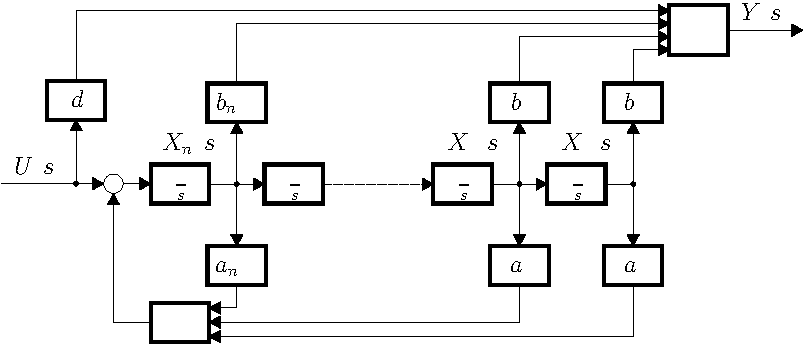
\includegraphics[width=0.75\columnwidth]{images/ZRD_regelungsnormalform.pdf}
\end{center}

In den Zeitbereich transformiert ergibt sich folgende Zustandsraumdarstellung:

$$
\overbrace{
\begin{bmatrix}
    \dot{x}_1 \\ \dot{x}_2 \\ \vdots \\ \dot{x}_{n-1} \\ \dot{x}_n
\end{bmatrix}
}^{\dot{x}}
=
\overbrace{
\begin{bmatrix}
    0       & 1         & 0         & \cdots    & 0         \\
    0       & 0         & 1         & \ddots    & \vdots    \\
    \vdots  & \vdots    & \ddots    & \ddots    & 0         \\
    0       & 0         & \cdots    & 0         & 1         \\
    -a_0    & -a_1      & \cdots    & -a_{n-2}  & -a_{n-1}
\end{bmatrix}
}^{A}
\cdot 
\overbrace{
\begin{bmatrix}
    x_1 \\ x_2 \\ \vdots \\ x_{n-1} \\ x_n
\end{bmatrix}
}^{x}
+
\overbrace{
\begin{bmatrix}
    0 \\ 0 \\ \vdots \\ 0 \\ 1
\end{bmatrix}
}^{b} \cdot  u
$$

$$
y =
\underbrace{
\begin{bmatrix}
    b_0 & b_1 & \cdots & b_{n-2} & b_{n-1}
\end{bmatrix}
}_{c}
\begin{bmatrix}
    x_1 \\ x_2 \\ \vdots \\ x_{n-1} \\ x_n
\end{bmatrix}
+ d \cdot u
$$


\subsubsection{Eindeutigkeit}

\begin{outline}
    \1 Aus einer UTF eine Zustandsraumdarstellung zu gewinnen ist \textbf{nicht eindeutig}. Auf triviale Art lassen sich alternative Formen
        produzieren (z.B. Zustandsvariablen anders nummerieren)
    \1 Aus einer ZRD die UTF zu gewinnen ist \textbf{eindeutig}
\end{outline}


\subsection{ZRD im Bildbereich}



\begin{minipage}[c]{0.5\columnwidth}
    Die ZRD existiert auch im Bildbereich und hat die Form:
\end{minipage}
\hfill
\begin{minipage}[c]{0.45\columnwidth}
        \fbox{\parbox{0.9\columnwidth}{
            \vspace{-0.3cm}
            \begin{align*}
                s X(s)  &= \bm{A} \cdot X(s) + \bm{B} \cdot U(s) + x(0) \\
                Y(s)    &= \bm{C} \cdot X(s) + \bm{D} \cdot U(s)
            \end{align*}
            \vspace{-0.5cm}
    }}
\end{minipage}


\subsubsection{UTF aus ZRD (Bildbereich)}

\vspace{-0.3cm}

\begin{minipage}[c]{0.44\columnwidth}
    Die UTF $G(s)$ kann durch den Zusammenhang rechts gewonnen werden.

    \smallskip

    \textbf{Hinweis:} In der UTF $G(s)$ kommen keine (statischen) Zustände $x_0$ mehr vor.
\end{minipage}
\hfill
\begin{minipage}[c]{0.52\columnwidth}
    \begin{align*}
        Y(s)    &= \bm{C} \cdot \overbrace{(s \bm{I} - \bm{A})^{-1} \cdot \bm{B} \cdot U(s)}^{X(s)} + \bm{D} \cdot U(s)  \\
                &= \underbrace{\left[ \bm{C} \cdot (s \bm{I} - \bm{A})^{-1} \cdot \bm{B} + \bm{D} \right]}_{G(s)} \cdot U(s)
    \end{align*}
\end{minipage}


\subsection{Zustandsraumdarstellung aus Blockdiagramm}{171}
\label{Zustandsraumdarstellung aus Blockdiagramm}

Mittels folgendem Vorgehen kann die ZRD aus dem Blockdiagrmam bestimmt werden:

\smallskip
\begin{enumerate}
    \item Eingangs- und Ausgangssignale bestimmen
    \item Zustandsvektor bilden, indem alle Speicher aufgelistet werden \\
        \textrightarrow\ Länge des Zustandsvektors entspricht Systemordnung \\
        \textrightarrow\ entspricht Summe der Ordnung der Teilsysteme
    \item Gleichung $\dot{x} = f(x, u)$ bilden, indem alle Intergratoreingänge $(=\dot{x}_i)$ 'zurückverfolgt' werden,
        bis deren Abhängigkeit von Eingangssignalen \& Zustandsvariablen definiert ist
    \item Gleichung $y = g(x, u)$ bilden, indem Ausgangssignale $(=y_i)$ 'zurückverfolgt' werden, bis deren Abhängigkeit von 
        Eingangssignalen \& Zustandsvariablen definiert ist
    \item Bei linearen Systemen: Gleichungen $f$ und $g$ mit Matritzen $\bm{A}, \, \bm{B}, \, \bm{C}$ und $\bm{D}$ formulieren
\end{enumerate}

\vspace{-0.1cm}

\textbf{Beim Ausgang anfangen und Integrator für Integrator in Richtung Eingang wandern. 
Für jeden 'Block' eine Gleichung aufstellen und diese in ZRD 'einfüllen'}


\example{ZRD aus Blockdiagramm}

\begin{minipage}[c]{0.53\columnwidth}
    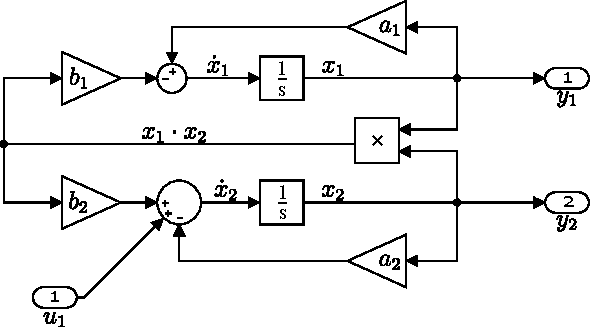
\includegraphics[width=\columnwidth]{images/ZRD_beispiel_blockdiagramm.pdf}
\end{minipage}
\hfill
\begin{minipage}[c]{0.45\columnwidth}
    \resizebox{\columnwidth}{!}{
        \renewcommand{\arraystretch}{1.3}
        \begin{tabular}{@{}ll@{}}
            $\dot{x}_1(t) = f_1(x, u)$  & $= a_1 \cdot x_1(t)$                      \\
                                        & $\quad - b_1 \cdot x_1(t) \, x_2(t)$            \\
            $\dot{x}_2(t) = f_2(x, u)$  & $= -a_2 \cdot x_2(t)$                     \\
                                        & $\quad + b_2 \cdot x_1(t) \, x_2(t) + u_1(t)$   \\
            $y_1(t) = g_1(x, u)$        & $= x_1(t)$                                \\
            $y_2(t) = g_2(x, u)$        & $= x_2(t)$
        \end{tabular}
        \renewcommand{\arraystretch}{1}
    }
\end{minipage}



\subsection{Blockdiagramm aus ZRD / Gleichung}

%NOTE: Nicht im Skirpt, kurz in V3 von Kottmann erwähnt

\begin{itemize}
    \item Auflösen nach höchster Ableitung
    \item Kette von Integratoren aufzeichnen
    \item Signale nach Integratoren wie benötigt abgreifen und Gleichung 'zusammenbauen'
\end{itemize}


\subsection{Aggregation von Teilsystemen}{172-174}
\label{Aggregation von Teilsystemen}

\textbf{Hinweis:} Grossbuchstaben und fett gedrucktes sind Matritzen


\begin{minipage}[t]{0.52\columnwidth}
    \subsubsection{Serieschaltung}

    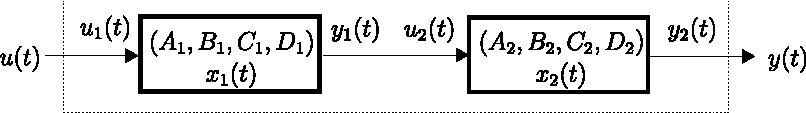
\includegraphics[width=\columnwidth]{images/ZRD_serieschaltung.pdf}
    $$
    \overbrace{ \begin{bmatrix} \dot{x}_1 \\ \dot{x}_2 \end{bmatrix}}^{\dot{x}}
    =
    \overbrace{\begin{bmatrix} A_1 & 0 \\ B_2 \cdot C_1 & A_2 \end{bmatrix} }^{\bm{A}}
    \cdot
    \overbrace{ \begin{bmatrix} x_1 \\ x_2 \end{bmatrix} }^{x}
    +
    \overbrace{ \begin{bmatrix} B_1 \\ B_2 \cdot D_1 \end{bmatrix} }^{\bm{B}} \cdot u
    $$
    $$
    y =
    \underbrace{ \begin{bmatrix} D_2 \cdot C_1 & C_2 \end{bmatrix}}_{\bm{C}}
    \cdot
    \underbrace{ \begin{bmatrix} x_1 \\ x_2 \end{bmatrix} }_{x}
    +
    \underbrace{D_2 \cdot D_1}_{\bm{D}} \cdot u
    $$
\end{minipage}
\hfill
\begin{minipage}[t]{0.45\columnwidth}
    \subsubsection{Parallelschaltung}

    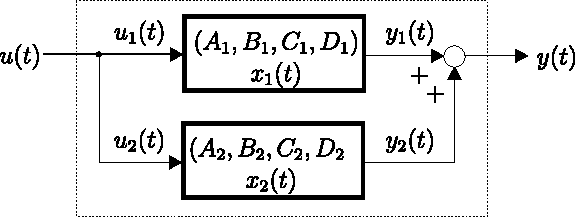
\includegraphics[width=\columnwidth]{images/ZRD_parallelschaltung.pdf}
    $$
    \overbrace{ \begin{bmatrix} \dot{x}_1 \\ \dot{x}_2 \end{bmatrix} }^{\dot{x}}
    =
    \overbrace{ \begin{bmatrix} A_1 & 0 \\ 0 & A_2 \end{bmatrix}}^{\bm{A}}
    \cdot 
    \overbrace{ \begin{bmatrix} x_1 \\ x_2 \end{bmatrix} }^{x}
    +
    \overbrace{ \begin{bmatrix} B_1 \\ B_2 \end{bmatrix} }^{\bm{B}} \cdot u
    $$
    $$
    y =
    \underbrace{ \begin{bmatrix} C_1 & C_2 \end{bmatrix} }_{\bm{C}}
    \cdot
    \underbrace{ \begin{bmatrix} x_1 \\ x_2 \end{bmatrix} }_{x}
    +
    \underbrace{(D_2 + D_1)}_{\bm{D}} \cdot u
    $$
\end{minipage}



\subsubsection{Kreisschaltung}


\begin{minipage}[c]{0.55\columnwidth}
    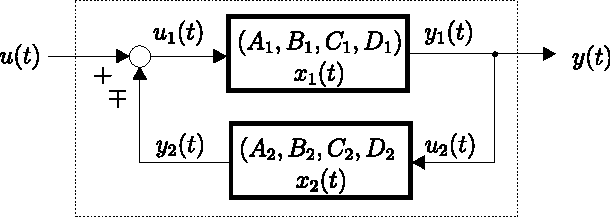
\includegraphics[width=\columnwidth]{images/ZRD_kreisschaltung.pdf}
\end{minipage}
\hfill
\begin{minipage}[c]{0.42\columnwidth}
    $$ K_1 = (I \pm D_2 D_1)^{-1} $$
    $$ K_2 = (I \pm D_1 D_2)^{-1} $$

    \begin{center}
        SISO-Systeme: $K_1 = K_2$
    \end{center}
\end{minipage}

\smallskip

$$
\overbrace{ \begin{bmatrix} \dot{x}_1 \\ \dot{x}_2 \end{bmatrix} }^{\dot{x}}
=
\overbrace{
\begin{bmatrix}
    A_1 \mp B_1 K_1 D_2 C_1 & \mp B_1 K_1 C_2           \\
    B_2 K_2 C_1             & A_2 \mp B_2 K_2 D_1 C_2
\end{bmatrix}}^{\bm{A}}
\cdot 
\overbrace{ \begin{bmatrix} x_1 \\ x_2 \end{bmatrix} }^{x}
+
\overbrace{
\begin{bmatrix} B_1 K_1 \\ B_2 K_2 D_1 \end{bmatrix} }^{\bm{B}} u
$$
$$
y =
\underbrace{ \begin{bmatrix} K_2 C_1 & \mp K_2 D_1 C_2 \end{bmatrix} }_{\bm{C}}
\cdot
\underbrace{ \begin{bmatrix} x_1 \\ x_2 \end{bmatrix} }_{x}
+
\underbrace{K_2 D_1}_{\bm{D}} \cdot u
$$

\columnbreak


\subsection{Ähnlichkeitstransformation}{175}
\label{Ähnlichkeitstransformation}


Bei der Ähnlichkeitstransformation wird eine ZRD in eine andere ZRD transformiert,
welche \textbf{dasselbe I/O-Verhalten}, aber einen \textbf{anderen internen Zustandsvektor} hat. \\
Die Ähnlichkeitstransformation wird verwendet, um ein System in eine 'besser geeignete' Form zu bringen.

\vspace{-0.2cm}

\begin{minipage}[c]{0.3\columnwidth}
    $$ \dot{x}(t) =\bm{A} \cdot x(t) + \bm{B} \cdot u(t) $$
    $$ y(t) =\bm{C} \cdot x(t) + \bm{D} \cdot u(t) $$
\end{minipage}
\hfill
\begin{minipage}[c]{0.38\columnwidth}
    $$ \underrightarrow{\text{Ähnlichkeitstransformation}} $$
\end{minipage}
\hfill
\begin{minipage}[c]{0.3\columnwidth}
    $$ \dot{\tilde{x}}(t) =\bm{\tilde{A}} \cdot \tilde{x}(t) + \bm{\tilde{B}} \cdot u(t) $$
    $$ y(t) =\bm{\tilde{C}} \cdot \tilde{x}(t) + \bm{\tilde{D}} \cdot u(t) $$
\end{minipage}

\medskip

Wenn der Zustand $x(t)$ mit einer \textbf{regulären konstanten Matrix} $\bm{P}$ multipiziert wird, ergibt sich der neue 
Zustand $\tilde{x}(t)$.
Die Umrechnungen (Ähnlichkeitstransformation) der ZRD erfolgt allgemein mittels.
$$ \boxed{ \tilde{x} = \bm{P} x \qquad  \bm{\tilde{A}} = \bm{P A P^{-1}} \qquad \bm{\tilde{B}} = \bm{P B} \qquad \bm{\tilde{C}} = \bm{C P^{-1}} \qquad \bm{\tilde{D}} = \bm{D} } $$


\subsubsection{Eigenschaften der Ähnlichkeitstransformation}

\begin{outline}
    \1 Direkte I/O-Kopplung ($\bm{\tilde{D}} = \bm{D}$) bleibt wegen gleichem I/O-Verhalten unverändert
    \1 Ändert Eigenwerte der Matix \textbf{nicht}
    \1 Ändert \textbf{nichts} an Steuerbarkeit, Beobachtbarkeit und Minimalität eines Systems
    \1 Um z.B. in einer Simulation die korrekten Signalverläufe zu berechnen, muss eine Anfangsbedingung mittransformiert werden: $\tilde{x}(0) = \bm{P} \cdot x(0)$
    \1 Wird ein System mit $\bm{P_1} = \bm{P}$ transformiert und das resultierende System mit $\bm{P_2} = \bm{P^{-1}}$ rücktransformiert, so ergibt isch wieder das ursprüngliche System
\end{outline}


\example{Zustandsvariablen in ZRD tauschen}

\begin{minipage}[c]{0.48\columnwidth}
    Eine gegebene ZRD mit Zustandsvektor $x$ soll mit Zustandsvektor $\tilde{x}$ ausgedrückt werden.
    Dafür wird die Transformationsmatrix $\bm{P}$ benötigt.
\end{minipage}
\hfill
\begin{minipage}[c]{0.48\columnwidth}
    $$ \text{ \textrightarrow } \quad \tilde{x} = \begin{bmatrix} \tilde{x}_1 \\ \tilde{x}_2 \end{bmatrix} = \begin{bmatrix} x_2 \\ x_1 \end{bmatrix}
    = \underbrace{ \begin{bmatrix} 0 & 1 \\ 1 & 0 \end{bmatrix} }_{ \bm{P} } \cdot \underbrace{ \begin{bmatrix} x_1 \\ x_2 \end{bmatrix} }_{ x } $$
\end{minipage}
%-----------------------------------------------------------------------------------------------------------------------------------
\para{Vertauschen von Zuständen}

Für

\[
\tilde x=
\begin{bmatrix}
x_2\\
x_1
\end{bmatrix}
\]

gilt

\[
P=
\begin{bmatrix}
0&1\\
1&0
\end{bmatrix}
\]

und

\[
\tilde A=PAP^{-1},
\qquad
\tilde B=PB,
\qquad
\tilde C=CP^{-1}
\]
%-----------------------------------------------------------------------------------------------------------------------------------
        \section{Anwendungen der ZRD}

\subsection{Lösung der ZRD im Zeitbereich}{176-180}
\label{ZRD Lösung Zeitbereich}


Durch eine Transformation der ZRD in den Frequenzbereich, algebraische Berechnungen und anschliessender Rücktransformation in den Zeitbereich
ergibt sich die \textbf{Lösung der ZRD im Zeitbereich} als:

\vspace{-0.2cm}

\begin{empheq}[box=\fbox]{align*}
    x(t) &= \underbrace{ e^{\bm{A} t} \cdot x_0}_{x_F} + \underbrace{ \int\limits_0^t e^{\bm{A} (t - \tau)} \cdot \bm{B} \cdot u(\tau) \, \diff \tau }_{x_E} \\
    y(t) &= \underbrace{ \bm{C} \cdot e^{\bm{A} t} \cdot x_0 }_{y_F} + \underbrace{ \bm{C} \cdot \int\limits_0^t  \e^{\bm{A} (t - \tau)} \cdot \bm{B} \cdot u(\tau) \, \diff \tau + \bm{D} \cdot u(t)}_{y_E}
\end{empheq}


\begin{tabular}{ll}
    $x_F$   & Freie Antwort: System mit $u = 0$ aus Anfangszustand $x_0 = x(0)$ loslassen   \\
    $x_E$   & Erzwungene Antwort: System aus Zustand $x_0 = 0$ loslassen                    \\
            & \textrightarrow\ nur abhängig von Eingangssignal $u$
\end{tabular}

\smallskip

\textbf{Hinweis:} $e^{\bm{A} t} = \bm{\Phi}(t)$ heisst \textbf{Transitionsmatrix} \textrightarrow\ siehe Abschnitt \ref{Transitionsmatrix}

\medskip


\paragraph{Eigenschaften -- Freie Antwort}

Für die freie Antwort ergeben sich aus der Theorie der Eigenwerte / Eigenvektoren die folgenden Eigenschaften:

\begin{outline}
    \1 Zeigt der Startwert $x_0 = v_i$ in die Richtung eines Eigenvektors, so bewegt sich der Zustand ausschliesslich in diese Richtung:
        $x(t) = e^{\lambda_i t} \cdot v_i = e^{\lambda_i t} \cdot x_0$
    \1 Zeigt $x_0$ in eine beliebige Richtung, so kann $x(t)$ durch Superposition bestimmt werden
        \2 $x_0$ wird in Richtung der Eigenvektoren $v_i$ zerlegt und jede dieser Komponenten folgt bei der zeitlichen Entwicklung dem Faktor $e^{\lambda_i t}$
\end{outline}



\subsubsection{Impulsantwort $\boldsymbol{g(t)}$}

Ist die Transitionsmatrix $e^{\bm{A} t} = \bm{\Phi}(t)$ bekannt, so ist die \textbf{Impulsantwort $g(t)$}
$$ \boxed{ g(t) = \bm{C} \cdot e^{\bm{A} t} \cdot \bm{B} + \bm{D} \cdot \delta(t) = \bm{C} \cdot \bm{\Phi}(t) \cdot \bm{B} + \bm{D} \cdot \delta(t) } $$


\subsection[Transitionsmatrix]{Transitionsmatrix $e^{\bm{A} t} = \bm{\Phi}$}{177}
\label{Transitionsmatrix}

\begin{minipage}[c]{0.7\columnwidth}
    \raggedright
    Die Transitionsmatrix (auch Fundamentalmatrix genannt) ist (wie oben bereits angewandt) definiert als:
\end{minipage}
\hfill
\begin{minipage}[c]{0.28\columnwidth}
    \raggedright
    $$ \boxed{ e^{\bm{A} t} = \bm{\Phi}(t) } $$
\end{minipage}

\smallskip

Sie wird benötigt, um die Zustandsraumdarstellung im \textbf{Zeitbereich} zu lösen.
Es gibt grundsätzlich mehrere Methoden, die quadratische $(n \times n)$ Transitionsmatrix zu bestimmen.

\smallskip

Hier soll allerdings die analytische Berechnung mittels inverser Laplace-Transformation erwähnt sein:
$$ \boxed{ \bm{\Phi}(t) = e^{\bm{A} t} = \mathcal{L}^{-1} \Bigl\{ (s \bm{I} - \bm{A})^{-1} \Bigr\} } $$

\textbf{Hinweis:} Die Rücktransformation erfolgt erst im letzten Schritt. \\
\textrightarrow\ Jedes Element der Matrix wird \textbf{einzeln} rücktransformiert


\medskip

\paragraph{Eigenschaften der Transitionsmatrix $\bm{\Phi}(t) = e^{\bm{A} t}$}

\smallskip

\begin{ctabular}{c | c | c}
    $\bm{\Phi}(0) = \bm{I}$ & $\bm{\dot{\Phi}}(t) = \bm{A} \cdot \bm{\Phi}(t) \, (= \bm{\Phi}(t) \cdot \bm{A})$ & $\bm{\Phi}(t)$ ist stets invertierbar
\end{ctabular}



\paragraph{Transitionsmatrix einer Diagonalmatrix}

Die Transitionsmatrix $\bm{\Phi}(t) = e^{\bm{A} t}$ kann eifach berechnet werden, wenn $\bm{A}$ eine Diagonalmatrix ist.

$$
\bm{A_{\rm Diag}} = 
\begin{bmatrix}
    \lambda_1   & 0     \\
    0           & \lambda_2 
\end{bmatrix} 
\qquad \Rightarrow\ \quad
e^{\bm{A_{\rm Diag}} t} = 
\begin{bmatrix}
    e^{\lambda_1 t} & 0                 \\
    0               & e^{\lambda_2 t}
\end{bmatrix} 
$$

\textbf{Hinweis:} Diagonalisierung einer Matrix: siehe Abschnitt \ref{Diagonalisierung}


\subsection{Entkopplung mittels Diagonalform}{180-185}

Die Diagonalform entkoppelt die $n$ Differentialgleichunge 1. Ordnung der ZRD, sodass man $\bm{n}$ \textbf{voneinander unabhängige} Differentialgleichungen erhält.

\smallskip

Die Lösung der Zustandsgleichungen (bzw. der ZRD) ist besonders einfach, wenn sich das System in \textbf{Diagonalform} befindet.
Ausserdem ist die \textbf{Stabilität} des Systems sofort an der \textbf{Diagonalmatrix} $\bm{\Lambda} = \bm{A_{\rm Diag}}$ ablesbar.

\smallskip

Für ein \textbf{SISO-System} ist die Diagonalform gegeben als:


\begin{minipage}[t]{0.5\columnwidth}
    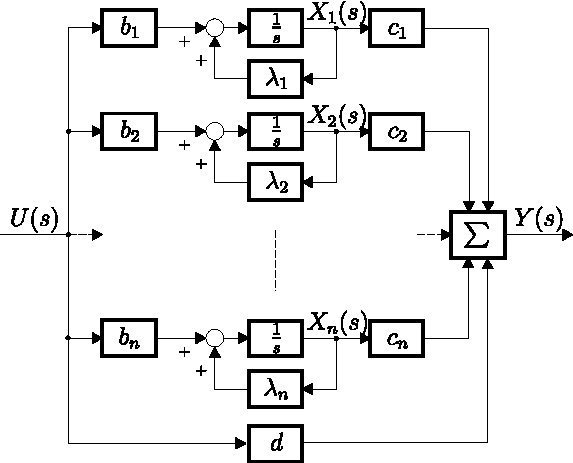
\includegraphics[width=\columnwidth, align=t]{images/ZRD_diagonalform.pdf}
\end{minipage}
\hfill
\begin{minipage}[t]{0.48\columnwidth}

    \vspace{-0.2cm}

    $$
    \begin{bmatrix}
        \dot{x}_1 \\
        \dot{x}_2 \\
        \vdots \\
        \dot{x}_n
    \end{bmatrix}
    =
    \overbrace{
    \begin{bmatrix}
        \lambda_1   & 0         & \cdots    & 0         \\
        0           & \lambda_2 & \ddots    & \vdots    \\
        \vdots      & \ddots    & \ddots    & 0         \\
        0           & 0         & \cdots    & \lambda_n
    \end{bmatrix}
    }^{\bm{\Lambda} = \bm{A_{\rm Diag}}}
    \begin{bmatrix}
        x_1 \\
        x_2 \\
        \vdots \\
        x_n
    \end{bmatrix}
    +
    \begin{bmatrix}
        b_1 \\
        b_2 \\
        \vdots \\
        b_n
    \end{bmatrix}
    \cdot u
    $$
    $$
    y =
    \begin{bmatrix}
        c_1 & c_2 & \dots & c_n
    \end{bmatrix}
    \cdot
    \begin{bmatrix}
        x_1 \\
        x_2 \\
        \vdots \\
        x_n
    \end{bmatrix}
    + d \cdot u
    $$
\end{minipage}
    

Aus dem Diagramm ist ersichtlich, dass das System folgende UTF $G(s)$ hat:

$$ G(s) = \frac{Y(s)}{U(s)} = \frac{b_1 c_1}{s - \lambda_1} +  \frac{b_2 c_2}{s - \lambda_2} + \cdots + \frac{b_n c_n}{s - \lambda_n} $$


\paragraph{Eigenschaften der Diagonalform}

\begin{outline}
    \1 Wenn $G(s)$ \textbf{minimal} ist, entsprechen die Diagonal-Elemente $\lambda_i$ der Systemmatrix $\bm{\Lambda} = \bm{A_{\rm diag}}$ den \textbf{Polen} von $G(s)$, also den Polen der $n$ parallelen $\text{PT}_1$-Glieder
        \2 'Interne' Stabilität' kann bei nicht-minimalen Systemen von I/O-Stabilität der UTF $G(s)$ abweichen
     \1 $G(s)$ ist \textbf{minimal}, bzw. hat Ordnung $n$, wenn
        \2 alle Produkte $b_i c_i \neq 0$ sind \textbf{und}
        \2 alle Pole unterschiedlich sind, d.h. $\lambda_i \neq \lambda_j$ für $i \neq j$
    \1 Gut geeignet für Stabilitätsbetrachtung (siehe Abschnitt \ref{Stabilität})
\end{outline}



\subsection{Diagonalisierung}{182-185}
\label{Diagonalisierung}

\subsubsection{Diagonalisierung mittels PBZ}

Da die Diagonalmatrix $\bm{\Lambda} = \bm{A_{\rm Diag}}$ die Pole beinhaltet, können diese aus der UTF mittels PBZ berechnet werden und
anschliessend in eine Diagonalmatrix geschrieben werden. \\
\textbf{Diese Methode ist nur für SISO-Systeme anwendbar!}

\smallskip

\begin{outline}
    \1 Wenn Pol-/Nullstellenkürzungen möglich sind resultiert ebenfalls eine Diagonalstruktur, jedoch mit reduzierter Ordnung
    \1 Bei Mehrfachpolen resultiert die Jordanform
        \2 weicht geringfügig von Diagonalform ab
\end{outline}


\example{Diagonalisierung mittels PBZ}

\vspace{-0.3cm}

\begin{minipage}[b]{0.45\columnwidth}
    $$ G(s) =  \frac{s+3}{(s+1) (s+2)} = \frac{2}{s+1} + \frac{1}{s+2} $$
\end{minipage}
\hfill
\begin{minipage}[b]{0.18\columnwidth}
    $$ \underrightarrow{ \text{Pole in Matrix} } $$
\end{minipage}
\hfill
\begin{minipage}[c]{0.3\columnwidth}
    $$
    \bm{\Lambda} = \bm{A_{\rm Diag}} = 
    \begin{bmatrix}
        -1  & 0     \\
        0   & -2    \\
    \end{bmatrix}
    $$
\end{minipage}



\subsubsection{Diagonalisierung mittels Eigenwerten / Eigenvektoren}

Eine andere Methode der Diagonalisierung benutzt die Theorie der Eigenwerte und Eigenvektoren, welche auch für MIMO-Systeme angewendet werden kann.
Die Diagonalmatrix $\bm{\Lambda} = $ berechnet sich als

\vspace{-0.2cm}

$$ \boxed{ \bm{\Lambda} = \bm{A_{\rm Diag}} = \bm{V}^{-1} \cdot \bm{A} \cdot \bm{V} \qquad \quad \bm{V} = \text{Matrix der Eigenvektoren} } $$

\textrightarrow\ Entspricht Ähnlichkeitstransformation von $\bm{A}$ mit Transformationsmatrix $\bm{P} = \bm{V^{-1}}$


\subsection{Stabilität}
\label{Stabilität}

Ein LZI-System ist \textbf{asymptotisch stabil}, wenn \textbf{alle Pole in der linken Halbebene liegen} (bzw. einen negativen Realteil haben). \\
Unter Betrachtung der ZRD wird diese Bedingung interpretiert als:
Wenn alle \textbf{Eigenwerte} der \textbf{Systemmatrix} $\bm{A}$ (welche den Eigenwerten von $\bm{\Lambda} = \bm{A_{\rm Diag}}$ entsprechen)
einen \textbf{negativen Realteil} besitzen, ist das System \textbf{asymptotisch stabil}.

\vspace{-0.2cm}

$$ \boxed{ \det(\lambda \cdot \bm{I} - \bm{A}) \overset{!}{=} 0 \qquad \rightarrow \forall \lambda \quad \mathrm{Re} \{ \lambda \} < 0 \qquad \text{ \textrightarrow\ System asymptotisch stabil}}  $$

\textbf{Achtung: Umgekehrt gilt diese Aussage nicht!} Ein asymptotisch stabiles LTI-System bedeutet \textbf{nicht}, 
dass alle Eigenwerte der Systemmatrix $\bm{A}$ des Systems einen negativen Realteil besitzen. \textrightarrow\ Pol-/Nullstellenkürzungen


\columnbreak


\subsection{Steuerbarkeit}{185-187}

Die Steuerbarkeit beschäftigt sich mit der Frage, ob (bzw. wie) der \textbf{Zustand $\bm{x}$ durch den Eingang $\bm{u}$ beeinflusst} werden kann.
Somit können z.B. instabile Pole weiter nach links geschoben werden, um ein instabiles System zu stabilisieren.

\medskip

\paragraph{Defintionen von Steuerbarkeit}

Beide Definitionen von Steuerbarkeit sind äquivalent.

\smallskip

\begin{enumerate}
    \item Ein System $(\bm{A}, \, \bm{B})$ ist steuerbar, wenn der Zustandsvektor $x$ mit geeignetem $u(t)$ in endlicher Zeit $T_e$ von jedem
            Anfangszustand $x(0)$ zu jedem Endzustand $x(T_e)$ gebracht werden kann.
    \item Ein System $(\bm{A}, \, \bm{B})$ ist steuerbar, wenn die Eigenwerte von $\bm{A} - \bm{BK}$ durch geeignete
            Wahl von $\bm{K}$ beliebig plaziert werden können.
\end{enumerate}



\subsubsection{Steuerbarkeitsmatrix $\bm{Q_S}$}
\label{Steuerbarkeitsmatrix}

Ein System ist \textbf{vollständig steuerbar}, wenn
\begin{outline}
    \1 Der \textbf{Rang} der Steuerbarkeitsmatrix $\bm{Q_S}$ der Ordnung $n$ des Systems entspricht
        \2 Die Matrix $\bm{Q_S}$ hat somit vollen Rang
    \1 Bei Single-Input-System: ($m = 1$): Die \textbf{Determinante} von $\bm{Q_S}$ \textbf{ungleich Null ist}
\end{outline}

\vspace{-0.1cm}

$$
\boxed{ 
\bm{Q_S} = 
\begin{bmatrix}
    \bm{B} & \bm{A B} & \bm{A^2 B} & \cdots & \bm{A^{n-1} B} 
\end{bmatrix}
\qquad \qquad \text{ Dimension: } n \times (n \cdot m)
}
$$


\begin{minipage}[c]{0.48\columnwidth}
    \begin{tabular}{ll}
        $\bm{A}$    & Systemmatrix ($n \times n$)   \\
        $\bm{B}$    & Eingangsmatrix ($n \times m$) \\
    \end{tabular}
\end{minipage}
\hfill
\begin{minipage}[c]{0.48\columnwidth}
    \begin{tabular}{ll}
        $n$         & Zustände \\
        $m$         & Eingänge \\
    \end{tabular}
\end{minipage}


\subsubsection{Nicht-steuerbare Systeme}

\begin{outline}
    \1 Gewisse Eigenwerte von $\bm{A} - \bm{BK}$ sind \textbf{nicht verschiebbar}
    \1 Anzahl der fixen Eigenwerte entspricht dem Defizit des Rangs von $\bm{Q_S}$
\end{outline}


\example{Typische nicht-steuerbare Systeme}

\begin{center}
    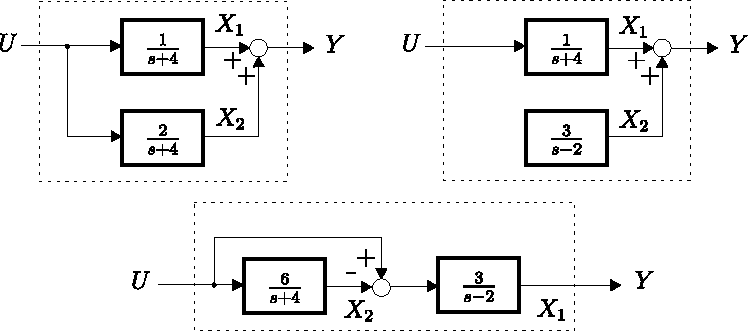
\includegraphics[width=0.8\columnwidth]{images/ZRD_nicht_steuerbare_systeme.pdf}
\end{center}


\subsubsection{Regelungsnormalform mittels Ähnlichkeitstransformation}

Ein steuerbares SISO-System kann mit einer geeigneten Transformationsmatrix $\bm{P}$ in Regelungsnormalform (siehe \ref{Regelungsnormalform}) 
gebracht werden. 


\begin{minipage}[c]{0.78\columnwidth}
    Diese geeigneten Transformationsmatrix $\bm{P}$ wird mittels folgendem Vorgehen ermittelt:

    \smallskip

    \begin{enumerate}
        \item Steuerbarkeitsmatrix $\bm{Q_S}$ invertieren   \\
            \textrightarrow\ Voraussetzung: muss invertierbar sein!
        \item Von $\bm{Q_S}^{-1}$ wird die letzte Zeile als $q$ bezeichnet
        \item Transformationsmatrix $\bm{P}$ bilden als
    \end{enumerate}
\end{minipage}
\hfill
\begin{minipage}[c]{0.2\columnwidth}
    $$
    \bm{P} =
    \begin{bmatrix}
        q                   \\
        q \cdot \bm{A}      \\
        q \cdot \bm{A}^2    \\
        \vdots              \\
        q \cdot \bm{A}^{n-1}
    \end{bmatrix}
    $$
\end{minipage}



\subsection{Beobachtbarkeit}{189}
\label{Beobachtbarkeit}

Die Beobachtbarkeit stellt die Frage danach, ob (bzw. wie) der \textbf{Zustand $\bm{x}$ durch die Messung des Ausgangs $\bm{y}$ bestimmt} werden kann.

\medskip

\paragraph{Defintionen von Beobachtbarkeit}

Beide Definitionen von Beobachtbarkeit sind äquivalent.

\smallskip

\begin{enumerate}
    \item Ein System $(\bm{A}, \bm{C})$ ist beobachtbar, wenn der Anfangszustand $x_0$ innert endlicher
        Zeit $T_e$ eindeutig bestimmt werden kann, sofern $u$ und $y$ für $0 \leq t \leq T_e$ bekannt sind.
    \item Ein System $(\bm{A}, \bm{C})$ ist beobachtbar, wenn die Eigenwerte von $\bm{A} - \bm{HC}$ durch geeignete
        Wahl von $\bm{H}$ beliebig plaziert werden können.
\end{enumerate}



\subsubsection{Beobachtbarkeitsmatrix $\bm{Q_B}$}
\label{Beobachtbarkeitsmatrix}

Ein System ist \textbf{vollständig beobachtbar}, wenn

\begin{outline}
    \1 Der \textbf{Rang} der Beobachtbarkeitsmatrix $\bm{Q_B}$ der Ordnung $n$ des Systems entspricht
        \2 Die Matrix $\bm{Q_B}$ hat somit vollen Rang
    \1 Bei Single-Output-System:  Die \textbf{Determinante} von $\bm{Q_B}$ \textbf{ungleich Null ist}
\end{outline}

\smallskip

\begin{minipage}[c]{0.4\columnwidth}
    $$
    \bm{Q}_B = 
    \begin{bmatrix}
        \bm{C} \\ \bm{C A} \\ \bm{C A^2} \\ \vdots \\ \bm{C A^{n-1}} 
    \end{bmatrix}
    $$
\end{minipage}
\hfill
\begin{minipage}[c]{0.58\columnwidth}
    \begin{tabular}{ll}
        Dimension:  & $(k \cdot n) \times n$ \\
        $\bm{A}$    & Systemmatrix ($n \times n$) \\
        $\bm{C}$    & Beobachtungsmatrix ($k \times m$) \\
        $n$         & Zustände \\
        $m$         & Eingänge \\
        $k$         & Ausgänge 
    \end{tabular}
\end{minipage}


\subsubsection{Nicht-beobachtbare Systeme}

\begin{outline}
    \1 Gewisse Eigenwerte von $\bm{A} - \bm{HC}$ sind \textbf{nicht verschiebbar}
    \1 Anzahl der fixen Eigenwerte entspricht dem Defizit des Rangs von $\bm{Q_B}$
\end{outline}


\example{Typische nicht-beobachtbare Systeme}

\begin{center}
    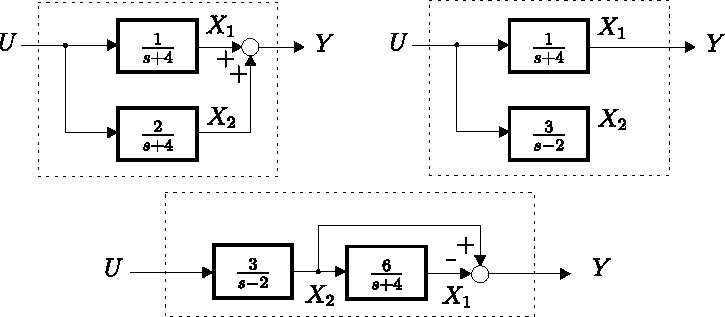
\includegraphics[width=0.8\columnwidth]{images/ZRD_nicht_beobachtbare_systeme.pdf}
\end{center}


\subsection{Minimalität}

Ein System ist minimal, wenn...
\begin{outline}
    \1 Das System \textbf{steuerbar und beobachtbar} ist
    \1 Keine Pol-/NS-Kürzungen in der UTF möglich sind
\end{outline}

% Ist ein System \textbf{steuerbar und beobachtbar}, so ist es minimal. In der UTF können keine Pol-/NS-Kürzungen vorgenommen werden.

\smallskip

Zu einem nicht-minimalen System $(\bm{A}, \, \bm{B}, \, \bm{C})$ kann ein System $(\bm{A_M}, \, \bm{B_M}, \, \bm{C_M})$ tieferer Ordnung
angegeben werden, das trotzdem \textbf{dieselbe UTF}(-Matrix) $G(s)$ hat.

\subsubsection{Einfluss von Nichtminimalität}

\begin{outline}
    \1 \textbf{Bau eines neuen Systems}
        \2 Ersetzung durch minimale Version des Systems \\
        \textrightarrow\ Bau der \textbf{minimale Realisierung} des Systems
    \1 \textbf{Reglerentwurf für bestehende nichtminimale Strecke}
        \2 mindestens ein Pol (bzw. Eigenwert) der Strecke nicht veränderbar \\
            \textrightarrow\ \textbf{gravierend}, wenn Strecke deshalb nicht stabilisiert werden kann
        \2 Algorithmen / Softwarepakete funktionieren oft nicht korrekt, wenn System nicht minimal
\end{outline}



\subsection{Normalformen}

Kann ein SISO-System mit UTF $G(s)$ in eine der beschriebenen Normalformen gebracht werden, so hat das System gewisse Eigenschaften

$$  G(s) = d + \frac{b_{n-1} s^{n-1} + \cdots + b_1 s + b_0}{s^n + a_{n-1} s^{n-1} + \cdots + a_1 s +a_0 } $$


\subsubsection{Regelungsnormalform}{188}
\label{Regelungsnormalform}

Kann ein System in Regelungsnormalform gebracht werden, so ist es \textbf{immer steuerbar}.

$$
A =
\begin{bmatrix}
    0       & 1         & 0         & \cdots    & 0         \\
    0       & 0         & 1         & \ddots    & \vdots    \\
    \vdots  &           & \ddots    & \ddots    & \vdots    \\
    0       & 0         & \cdots   & 0         & 1         \\
    -a_0    & -a_1      & \cdots    & -a_{n-2}  & -a_{n-1}
\end{bmatrix}
\quad
b =
\begin{bmatrix}
    0 \\ 0 \\ \vdots \\ 0 \\ 1
\end{bmatrix}
\quad
c =
\begin{bmatrix}
    b_0 \\ b_1 \\ \vdots \\ b_{n-2} \\ b_{n-1}
\end{bmatrix}^{T}
\quad
d = d
$$



\subsubsection{Beobachtungsnormalform}

Kann ein System in Beobachtungsnormalform gebracht werden, so ist es \textbf{immer beobachtbar}.

$$
A =
\begin{bmatrix}
    0       & 0         & 0         & \cdots    & -a_0      \\
    1       & 0         & 0         & \cdots    & -a_1      \\
    0       & 1         & \ddots    & \ddots    & \vdots    \\
    \vdots  & \ddots    & \ddots    & 0         & -a_{n-2}  \\
    0       & \cdots    & 0         & 1         & -a_{n-1}
\end{bmatrix}
\quad
b =
\begin{bmatrix}
    b_0 \\ b_1 \\ \vdots \\ b_{n-2} \\ b_{n-1}
\end{bmatrix}
\quad
c =
\begin{bmatrix}
    0 \\ 0 \\ \vdots \\ 0 \\ 1
\end{bmatrix}^{T}
\quad
d = d
$$

\textbf{Hinweis:} Die Beobachtungsnormalform ist \textbf{dual} zur Regelungsnormalform.


\subsection{Eigenschaften von Zustandsraummodellen}{190-193}

Ausgewählte wichtige Eigenschaften eines Systems $(\bm{A}, \bm{B}, \bm{C})$ mit Zustandsvektor $x$ sind hier noch einmal aufgelistet:

\smallskip

\begin{outline}
    \1 Die Ordnung des Systems entspricht der Länge des Zustandsvektors $x$
    \1 System ist asymptotisch stabil, wenn alle Eigenwerte von $\bm{A}$ in der LHE liegen bzw. alle
        $\lambda_i < 0$ sind 
    \1 System ist steuerbar, wenn $\bm{Q_S}$ vollen Rang hat
    \1 System ist beobachtbar, wenn $\bm{Q_B}$ vollen Rang hat
        \2 Bei einem Beobachtbarkeits-Problem kann z.B. ein zusätzlicher Sensor die Strecke beobachtbar machen
    \1 Ein System ist minimal, wenn es steuerbar \textbf{und} beobachtbar ist
    \1 Wenn nur die UTF $G(s)$ eines Systems bekannt ist, sind \textbf{keine Aussagen über Steuerbarkeit / Beobachtbarkeit möglich} \\
        \textrightarrow\ Dafür muss innerer Aufbau des Systems (ZRD) bekannt sein!
\end{outline}




        \section{Zustandsrückführungen}

\begin{minipage}[t]{0.48\columnwidth}
    Bei einer Zustandsrückführung geht man davon aus, dass der Zustandsvektor $x$ des Systems vollständig bekannt ist und zur 
    Regelung benutzt werden kann.

    \smallskip

    \textbf{Hinweis:} Für die folgenden Betrachtungen des Systems gilt $\bm{D} = 0$, sowie

    \vspace{-0.2cm}

    $$
    \bm{K} = 
    \begin{bmatrix}
        k_1 &   k_2 & \ldots    & k_n
    \end{bmatrix}
    $$
\end{minipage}
\hfill
\begin{minipage}[t]{0.48\columnwidth}
    
    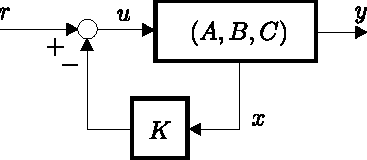
\includegraphics[width=\columnwidth, align=t]{images/ZRD_zustandsrueckfuehrung.pdf}
\end{minipage}

\medskip

\textbf{Hinweis:} Die Zeichnung zeigt das Konzept. In einem Blockdiagramm hat jede Zustandsgrösse ihre eine eigene Rückführung 
(und somit ihre eigene Verstärkung $k_i$)


Die Systemgleichung des geschlossenen Regelkreises mit \textbf{neuer Systemmatrix} $\overline{\bm{A}}$ ergibt sich zu:
$$ \dot{x} = \bm{A} \cdot x + \bm{B} \cdot u = \bm{A} \cdot x + \bm{B} \cdot \underbrace{(r - \bm{K} x)}_{u} = \underbrace{(\bm{A} - \bm{BK})}_{\overline{\bm{A}}} \cdot x + \bm{B} \cdot r $$

\medskip

Die UTF des geschlossenen Regelkreises $G_f(s)$ berechnet sich dann als:

\vspace{-0.2cm}

$$ G_f(s) = \frac{Y(s)}{R(s)} = \bm{C} \cdot (s \bm{I} - \bm{A} + \bm{BK})^{-1} \cdot \bm{B} = \bm{C} \cdot (s \bm{I} - \overline{\bm{A}})^{-1} \cdot \bm{B} $$

Wenn vorausgesetzt wird, dass das System $(\bm{A}, \, \bm{B})$ \textbf{steuerbar} ist, können die \textbf{Pole des geschlossenen Regelkreises beliebig vorgegeben} werden. \\
Dies kann mittels Polvorgabe (\ref{Polvorgabe}) oder LQR-Verfahren (\ref{LQR-Verfahren}) erreicht werden.
%-----------------------------------------------------------------------------------------------------------------------------------
\para{Geschlossener Kreis}

Für

\[
u=-Kx
\]

ergibt sich

\[
\dot x=(A-BK)x
\]

Die Eigenwerte von

\[
A-BK
\]

sind die Pole des geschlossenen Regelkreises.

\para{Polvorgabe}

Polplatzierung mittels Zustandsrückführung ist nur möglich, wenn

\[
\mathrm{rang}(Q_s)=n
\]

gilt.

\subsubsection{LQR-Regler}

Kostenfunktion:

\[
J=
\int_0^\infty
(x^TQx+u^TRu)\,dt
\]

Gewichte:

\[
Q \rightarrow Zustände
\]

\[
R \rightarrow Stellaufwand
\]

Regler:

\[
u=-Kx
\]

MATLAB:

\[
\texttt{k=lqr(A,B,Q,R)}
\]

\para{Vorverstärkung}

\[
u=-Kx+Lr
\]

\[
A_{cl}=A-BK
\]

Die Pole des geschlossenen Kreises sind die Eigenwerte von

\[
A-BK
\]
%-----------------------------------------------------------------------------------------------------------------------------------
\subsection{Eigenschaften von Zustandsrückführungen}

Reglenentwurf mittels Polvorgabe und LQR-Verfahren haben folgende Eigenschaften:

\smallskip

\begin{outline}
    \1 Zustandsrückführung wirkt sich nur auf \textbf{Pole} aus, nicht auf Nullstellen
        \2 Nullstellen, welche durch $b$-Koeffizienten bestimmt sind, belieben erhalten
    \1 Ordnung des Regelkreises bleibt erhalten ( \textrightarrow\ statischer Regler)
    \1 Zustandsrückführung $k$ entspricht grundsätzlichen einem statischen (P-)Regler.
        \2 Bei konstanter Führungsgrösse $r$ entsteht ein stationärer Fehler \\
            \textrightarrow\ kann durch Erweiterung mit Vorverstärkung oder I-Anteil in Regelkreis korrigiert werden (siehe Abschnitt \ref{Statische Erweiterungen der Zustandsrückführung})
\end{outline}


\subsection{Reglerentwurf mittels Polvorgabe}{194-196}
\label{Polvorgabe}

Bei der Zustandsrückführung können \textbf{alle $\bm{n}$ Pole beliebig vorgegeben} werden, sofern das \textbf{System steuerbar} ist.

\smallskip

Bei einer WOK hingegen hat man meist nur einen Freiheitsgrad (Verstärkungsfaktor des Reglers), um alle $n$ Pole festzulegen, 
da die Pollagen miteinander gekoppelt sind.


\subsubsection{Lage der Pole}

\begin{minipage}[t]{0.35\columnwidth}
    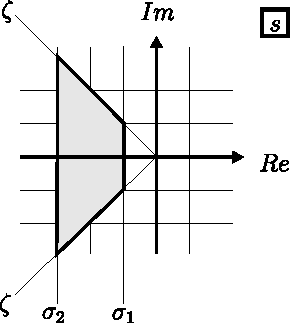
\includegraphics[width=\columnwidth, align=t]{images/ZRD_polplatzierung.pdf}
\end{minipage}
\hfill
\begin{minipage}[t]{0.62\columnwidth}
    \raggedright
    Die Wahl der Pole des Reglers soll folgende Kriterien erfüllen:

    \smallskip

    \begin{outline}
        \1 Pole müssen in LHE liegen $(\sigma < 0)$, damit Regelkreis stabil ist
        \1 Transienten sollen schneller abklingen als ein geeignetes $C \cdot e^{- \sigma_1}$
        \1 System soll genügend gedämpft sein, z.B. $\zeta > \frac{1}{\sqrt{2}}$
        \1 Obere Grenze $\sigma_2 > \sigma$ verhindert zu grosse Stellsignale
        \1 Pole, welche bereits akzeptabel liegen nicht unnötig verschieben
    \end{outline}
\end{minipage}


\subsubsection{Vorgabe der Pollagen}

Die Eigenwerte der Matrix $\overline{\bm{A}} = (\bm{A} - \bm{BK})$ sind gegeben durch die \textbf{Wurzeln} (Nullstellen) des Polynoms

\vspace{-0.2cm}

$$ \boxed{ \det \left(\lambda \cdot \bm{I} - \overline{\bm{A}} \right) = \det \left( \lambda \cdot \bm{I} - \bm{A} + \bm{BK} \right) = (\lambda - \lambda_1) \cdot  (\lambda - \lambda_2) \ldots  (\lambda - \lambda_n) } $$

Das geregelte System bzw. der geschlossene Regelkreis besitzt die UTF $G_f(s)$, bei welcher der \cbl{Nenner} bzw. die Pole vorgegeben werden.
$$ G_f(s)   = \frac{Y(s)}{U(s)} 
            = \frac{b_{n-1} s^{n-1} + b_{n-2} s^{n-2} + \ldots + b_1 s + b_0}{\cbl{ s^n + (a_{n-1} + k_n) s^{n-1} + \ldots + (a_1 + k_2) s + (a_0 + k_1) } } $$ 

Um die Pole des geregelten Systems $G_f(s)$ an die vorgegeben Stellen $\lambda_1 \ldots \lambda_n$ zu bringen, müssen folgende Polynome
mittels \textbf{Koeffizientenvergleich} zum Übereinstimmen gebracht werden. (Das Polynom rechts wird sinnvollerweise ausmultipliziert.)

\vspace{-0.2cm}

$$ \boxed{ \cbl{ s^n + (a_{n-1} + k_n) s^{n-1} + \ldots + (a_1 + k_2) s + (a_0 + k_1)} \overset{!}{=}
\det \left( s \cdot \bm{I} - \bm{A} + \bm{BK} \right) } $$

\textbf{Hinweis:} Die Parameter $k_i$ sind \textbf{eindeutig} bestimmbar, sofern das System \textbf{steuerbar} ist.


\example{Struktur eines Regelkreises mit Zustandsrückführung}

\begin{center}
    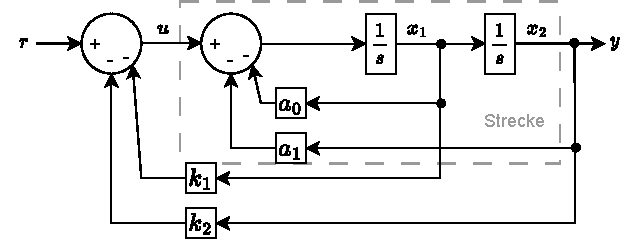
\includegraphics[width=0.7\columnwidth]{images/ZRD_zustandsrueckfuehrung_beispiel.pdf}
\end{center}

\vspace{-0.2cm}


\subsection{LQR-Verfahren (Linear Quadratic Regulator)}{196-199}
\label{LQR-Verfahren}

Für die Zustandsrückführungen wird die Matrix $\bm{K}$ mit Einträgen $k_i$ benutzt. Nun kann es sein, dass mehrere Matritzen $\bm{K}$ zur gleichen
Polverteilung führen. \\
\textrightarrow\ Das (Linear Quadratic Regulator) LQR-Verfahren ermittelt die \textbf{beste Matrix} $\bm{K}$

\medskip

Das LQR-Verfahren beruht auf der Lösung eines \textbf{Optimierungsproblems}. 
Aus folgenden beiden Anforderungen muss ein 'optimaler' Kompromiss gefunden werden:

\smallskip

\begin{outline}
    \1 Zustände $x(t)$ sollten möglichst schnell gegen $0$ konvergieren
    \1 Stellgrösse $u(t)$ soll nicht zu gross werden (nicht zu viel Stellenergie brauchen)
\end{outline}


\subsubsection{Zielfunktion $\bm{J(K)}$}

Die Zielfunktion $J(K)$ soll \textbf{minimiert} werden, um optimale Gewichtungsfaktoren $k_i$ für die Zustandsrückführungen zu finden. \\
Dabei setzt sich die Zielfunktion $J(K)$ aus den Zuständen $(x_1, \, \cdots, \, x_n)$ und den Eingangssignalen $(u_1, \, \cdots, \, u_m)$, 
sowie Gewichtungsmatritzen $\bm{Q}$ und $\bm{R}$ zusammen.

\begin{minipage}[c]{0.69\columnwidth}
    $$ \boxed{J(K) = \int\limits_{0}^{\infty} \left[ x(\bm{K}, t)^T \cdot\bm{Q} \cdot x(\bm{K}, t) + u(\bm{K}, t)^T \cdot \bm{R} \cdot u(\bm{K}, t) \right] \, \diff t } $$
\end{minipage}
\hfill
\begin{minipage}[c]{0.3\columnwidth}
    \begin{outline}
        \1 $\bm{Q}$ gewichtet Zustände \\
            Dimension: $n \times n$
            \smallskip
        \1 $\bm{R}$ gewichtet Eingänge \\
            Dimension: $m \times m$
    \end{outline}
\end{minipage}



\subsubsection{Wahl der Gewichtungsmatritzen $\bm{Q}$ und $\bm{R}$}

Die Matritzen $\bm{Q}$ und $\bm{R}$ werden folgendermassen gewählt:

\smallskip

\begin{outline}
    \1 Falls möglich: Diagonalmatritzen
        \2 Elemente auf \textbf{Diagonalen} müssen \textbf{positiv} sein \textrightarrow\ positiv definit
    \1 Falls keine Diagonalmatrix: Symmetrie
\end{outline}

\smallskip

\textbf{Hiweis:} In der Praxis ist die Wahl von $\bm{Q}$ und $\bm{R}$ meist ein \textbf{iterativer Prozess}. \\
Der 'erste Wurf' der Werte in den Matritzen wird so gewählt, dass \textbf{alle Summanden des Integranden in etwa gleich gewichtet} sind.


\example{Zielfunktion mit zwei Zuständen und einem Eingang}

Die Grössen liegen in den vorgegebene Bereichen.
Mit den Gewichtungsmatritzen sollen die Anteile der drei Integranden in vergleichbare Grösenordnungen gebracht werden.

\begin{ctabular}{l l l}
    \tabitem $x_1(t) \approx \pm 5 \cdot 10^{-3} \, \meter$         &
    \tabitem $x_2(t) \approx \pm 10^{2} \, \frac{\meter}{\second}$  &
    \tabitem $u(t) \approx \pm 10 \, \volt$
\end{ctabular}

\vspace{-0.3cm}

$$ \text{Integranden auf Gewichtung 1 bringen:} \quad \cbl{200^2} \cdot x_1^2 + \cor{100^2} \cdot x_2^2 + \cgn{0.1^2} \cdot u^2 $$

\vspace{-0.3cm}

\[
    \text{In Matrixform:} \quad 
    J = \int\limits_{0}^{\infty} \left[ x^T \cdot
    \begin{bmatrix}
        \cbl{4 \cdot 10^4}  & 0         \\
        0                   & \cor{10^4} 
    \end{bmatrix}
    \cdot x + u^T \cdot
    \begin{bmatrix}
        \cgn{10^{-2}}
    \end{bmatrix}
    \cdot u \right] \, \diff t
\]


\example{Nicht-Diagonale Matrix $\bm{Q}$}

Mischterme stehen neben der Diagonalen und werden aufgeteilt.

\vspace{-0.2cm}
\[
    \cbl{13} \cdot x_1^2 + \cvt{(-16)} \cdot x_1 \cdot x_2 + \cor{15} \cdot x_2^2
    \qquad 
    \Rightarrow\
    \begin{bmatrix}
        x_1 & x_2
    \end{bmatrix}
    \cdot
    \begin{bmatrix}
        \cbl{13}    & \cvt{-8}  \\
        \cvt{-8}    & \cor{15}
    \end{bmatrix}
    \cdot
    \begin{bmatrix}
        x_1 \\ x_2
    \end{bmatrix}
\]


\subsubsection{Optimale Rückführverstärkungen $\bm{K}$}

Der geschlossene Regelkreis mit Zustandsrückführung (also mit \textbf{neuer Systemmatrix} $\overline{\bm{A}}$) gehorcht der Differentialgleichung 

\vspace{-0.2cm}

$$ \dot{x} = \bm{A} \cdot x - \bm{BK} \cdot x = (\bm{A} - \bm{BK}) \cdot x \qquad \text{mit } x(0) = x_0 $$


und hat die Lösung

\vspace{-0.2cm}

$$ x(\bm{K}, t) = e^{(\bm{A} - \bm{BK}) t} \cdot x_0 \qquad \qquad
    u(\bm{K}, t) = - \bm{K} \cdot x(\bm{K}, t) = - \bm{K} \cdot e^{(\bm{A} - \bm{BK}) t} \cdot x_0 $$


\vspace{0.2cm}

Damit wird die Zielfunktion $\bm{J(K)}$ 

\vspace{-0.4cm}

\begin{align*}
    J(K)    &= \int\limits_{0}^{\infty} \left[ x(\bm{K}, t)^T \cdot\bm{Q} \cdot x(\bm{K}, t) + u(\bm{K}, t)^T \cdot R \cdot u(\bm{K}, t) \right] \, \diff t \\
            &= x_0^T \cdot \underbrace{ \int\limits_{0}^{\infty} \left[ e^{(\bm{A} - \bm{BK}) t} \right]^T \cdot \left[ \bm{Q} + \bm{K^T RK} \right] \cdot e^{(\bm{A} - \bm{BK}) t} \, \diff t }_{\bm{S}(\bm{K})} \cdot x_0
\end{align*}


Die optimalen Rückführverstärkungen (als Matrix $\bm{K}$) ergeben sich aus der positiv definiten Lösung der Matrix $\bm{S}$ der entsprechenden Matrix-Ricatti-Gleichung:

\vspace{-0.2cm}

$$ \boxed{ \bm{K} = \bm{R^{-1} B^T S} } $$

\textbf{Hinweis:} Meist wird die Lösung $\bm{K}$ direkt mit Matlab ermittelt.


\subsubsection{Eigenschaften des LQR-Verfahrens}

\begin{outline}
    \1 Ist $\bm{R}$ \textbf{'klein'}, ergibt sich tendentiell eine \textbf{grössere Reglerverstärkung $\bm{K}$} und ein schnellerer Regelkreis
        \2 Pole liegen weiter links
    \1 Werden $\bm{Q}$ und $\bm{R}$ um denselben Faktor geändert, so ergibt sich wieder dieselbe Rückführungsverstärkung $\bm{K}$
    \1 Gelegentlich ist es von Vorteil, als Gewichtung $\bm{Q} = \bm{C^T C}$ zu verwenden
        \2 $\bm{C}$ entspricht der 'richtigen' Ausgangsmatrix des Systems
    \1 Mittels LQR-Verfahren werden sehr \textbf{robuste Regler} entworfen (\textrightarrow\ siehe Skrip S. 199)
\end{outline}


\medskip

\paragraph{Einfluss von $\bm{R}$ und $\bm{Q}$ auf Stellgrösse $\bm{u(t)}$}

\begin{ctabular}{l c c}
    \toprule
    $\bm{R} \uparrow$ / $\bm{Q} \downarrow$ & $u(t=0) \, \downarrow$    & langsameres Abklinken \\
    \midrule
    $\bm{R} \downarrow$ / $\bm{Q} \uparrow$ & $u(t=0) \, \uparrow$      & schnelleres Abklinken \\
    \bottomrule
\end{ctabular}

%-----------------------------------------------------------------------------------------------------------------------------------
\subsubsection{Zustandsregler mit PI-Zusatz}

Integratorzustand:

\[
x_I=\int e(t)\,dt
\]

Erweiterter Zustandsvektor:

\[
x_{PI}
=
\begin{bmatrix}
x\\
x_I
\end{bmatrix}
\]

Regler:

\[
u=-Kx-k_Ix_I
\]

Vorteil:

\[
e_\infty = 0
\]

für konstante Führungs- und Störgrössen.
%-----------------------------------------------------------------------------------------------------------------------------------

\subsection{Statische Erweiterungen der Zustandsrückführung}
\label{Statische Erweiterungen der Zustandsrückführung}

Die Zustandsrückführung sorgt dafür, dass der geschlossene Regelkreis $G_f(s)$ eine befriedigende Dynamik hat.
Das (statische) \textbf{Folgeverhalten} ist jedoch noch \textbf{nicht garantiert}. \\
Für den geschlossenen Regelkreis $G_f(s)$ soll gelten:

\smallskip

\begin{outline}
    \1 Führungsverhalten: $y = r$
    \1 Keine Regelabweichung bei konstantem $r$: $e(t) = r(t) - y(t) \to 0$ bzw. $G_f(0) = 1$ 
\end{outline}

\smallskip

\textbf{Hinweis:} Folgende Betrachtungen beziehen sich auf SISO-Systeme.


\subsubsection{Erweiterung mit Vorverstärkung}{200}

$L$ kann verwendet werden, um $r = y$ zu garantieren. \\
Ausserdem kann $L$ als Vorfilter verwendet werden, und so die Dynamik des Regelkreises verbessern 
\textrightarrow\ Lead-Glied mit $T_2 < T_1$ macht Regelkreis schnell

\smallskip

\begin{minipage}[t]{0.63\columnwidth}
    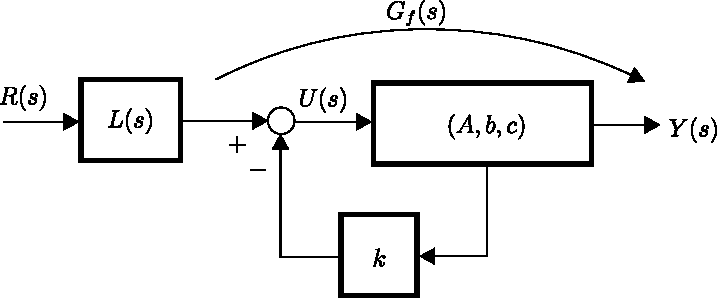
\includegraphics[width=\columnwidth, align=t]{images/zustandsrueckfuehrung_vorverstaerkung.pdf}
\end{minipage}
\hfill
\begin{minipage}[t]{0.33\columnwidth}
    \textbf{Verstärkung korrigieren:}
    $$ L = G_f(0)^{-1} = \frac{1}{G_f(0)} $$

    \textbf{Zusätzliches Vorfilter:}
    $$ L = \frac{1}{G_f(0)} \cdot \frac{s T_1 + 1}{s T_2 + 2} $$
\end{minipage}

\medskip

$$ \text{UTF Regelkreis (ohne  L(s)):} \quad G_f(s) = \frac{Y(s)}{U(s)} = \bm{C} \cdot (s \bm{I} - \bm{A} + \bm{BK})^{-1} \cdot \bm{B} = \bm{C} \cdot (s \bm{I} - \overline{\bm{A}})^{-1} \cdot \bm{B}$$

Die Vorverstärkung hat jedoch den \textbf{Nachteil der Parameterabhängigkeit}.


\subsubsection{Erweiterung mit PI- / I-Zusatz}{200-202}

Der statische Fehler kann auch mittels PI- bzw. reinem I-Anteil im Regler ($K_P = 0$) unterdrückt werden.
Der Entwurf eines solchen zusätzlichen Reglers kann auf zwei verschiedene Arten erfolgen.

\smallskip

Die Integratorerweiterung hat jedoch den \textbf{Nachteil der Phasensenkung}.

\medskip

\paragraph{Variante: Kaskadierter Regler}

Der Entwurf des Reglers erfolgt in zwei \textbf{separaten} Schritten:

\smallskip

\begin{enumerate}
    \item Zustandsrückführung $\bm{K}$ entwerfen
    \item PI-Regler für den in Schritt 1 entstandenen Regelkreis entwerfen
\end{enumerate}

\smallskip

\textrightarrow\ \textbf{Nicht ideal}, da z.B. die robusten Eigenschaften des inneren Kreises in Schritt 2) verloren gehen können

\vspace{-0.2cm}

\begin{center}
    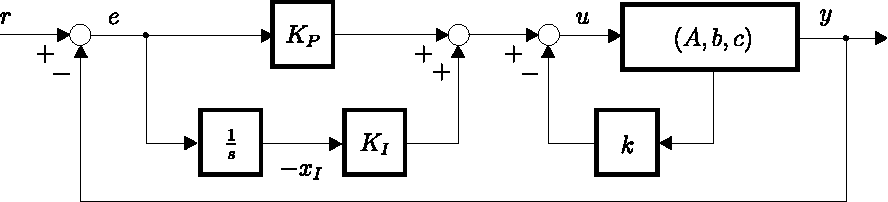
\includegraphics[width=0.8\columnwidth]{images/zustandsrueckfuehrung_PI.pdf}
\end{center}


\paragraph{Variante: Erweiterung der Strecke}

Eine bessere Variante ist es, den Regler 'aus einem Guss' zu entwerfen, indem die \textbf{Stecke} $n$-ter Orndung (aus obiger Abbildung)
\textbf{um einen Integrator erweitert} wird.

\smallskip

Der Zustandsvektor der neuen Strecke wird wegen dem zusätzlichen Integrator um den Zustand $x_I$ erweitert. Das System hat folgende ZRD:

\vspace{-0.1cm}

$$
\underbrace{ \begin{bmatrix} \dot{x} \\ \dot{x}_I \end{bmatrix}}_{\dot{x}_{\rm PI}}
=
\underbrace{\begin{bmatrix} \bm{A} & 0 \\ c & 0 \end{bmatrix} }_{\bm{A}_{\rm PI}}
\cdot
\underbrace{ \begin{bmatrix} x \\ x_I \end{bmatrix} }_{x_{\rm PI}}
+
\underbrace{ \begin{bmatrix} b \\ 0 \end{bmatrix} }_{b_{\rm PI}} \cdot u
\qquad \qquad 
y
=
\underbrace{ \begin{bmatrix} c & 0 \end{bmatrix}}_{c_{\rm PI}} \cdot x_{\rm PI}
$$


Für die neue Strecke kann anschliessend eine Zustandsrückführungsmatrix $\bm{K}$ ausgelegt werden. 
Dafür können Polplatzierung oder das LQR-Verfahren angewendet werden.

\vspace{-0.1cm}

$$ u = -(k + K_P \cdot c) \cdot c - K_I \cdot x_I = - \underbrace{ \begin{bmatrix} k + K_P \cdot c & K_I \end{bmatrix}}_{k_{\rm PI}} \cdot \underbrace{ \begin{bmatrix} x \\ x_I \end{bmatrix} }_{x_{\rm PI}} $$


\begin{outline}
    \1 Regler-Parameter $K_I$ entspricht letztem Element des Vektors $k_{\rm PI}$
    \1 Sobald der freie Parameter $K_P$ festgelegt ist, ist der Vektor $k_{\rm PI}$ eindeutig definiert
\end{outline}

\smallskip

Sobald die Werte $K_P$ und $K_I$ festgelegt sind, wird der Regler gemäss obiger \textbf{Kaskaden-Struktur} implementiert


        \section{Beobachter}

Für den Entwurf einer Zustandsrückführung ist es nötig, dass alle Zustandsgrössen $x$ gemessen werden können.
Dies ist oft nicht möglich oder zu teuer. \\
Stattdessen wird durch einen \textbf{Beobachter} (basierend auf dem \textbf{gemessenen Ausgangssignal} $y$) der gesamte \textbf{Zustandsvektor geschätzt}.
\textrightarrow\ Geschätzter Zustandsvektor: $\hat{x}(t)$

\smallskip

In der Struktur des Beobachter-System wird die Systemmatrix $\bm{A}$ durch die \textbf{neue Systemmatrix} $\overline{\bm{A}} = (\bm{A} - \bm{HC})$ ersetzt.
Ausserdem wird ein \textbf{Schätzfehler} $e = x - \hat{x}$ definiert, welcher gegen $0$ konvergieren soll.

\smallskip

Der Schätzfehler klingt vollständig ab, wenn der Realteil der Eigenwerte von $\overline{\bm{A}} < 0$ ist. 

\vspace{-0.2cm}

\begin{center}
    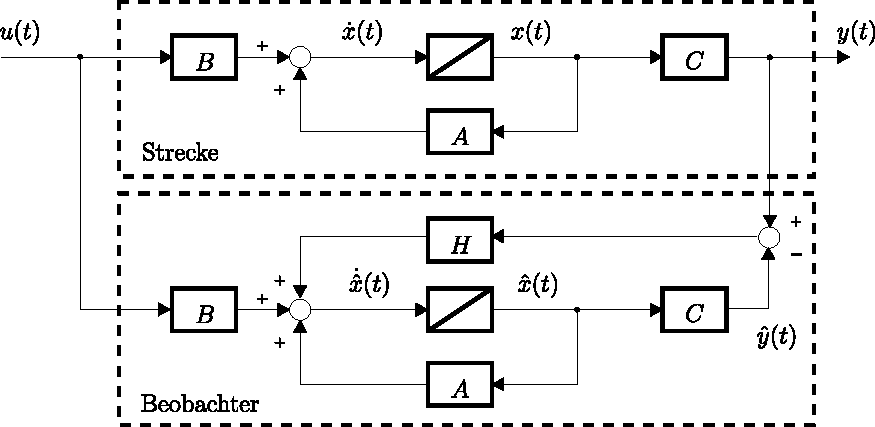
\includegraphics[width=0.85\columnwidth, align=t]{images/beobachter_strecke_mit_beobachter.pdf}
\end{center}


\textbf{Hinweis:} Für die folgenden Betrachtungen des Systems gilt $\bm{D} = 0$, sowie

\vspace{-0.1cm}

$$
\bm{H} = 
\begin{bmatrix}
        h_1 &   h_2 & \ldots    & h_n 
\end{bmatrix}^T
$$
%-----------------------------------------------------------------------------------------------------------------------------------

\para{Beobachterfehler}

\[
e=x-\hat x
\]

\[
\dot e=(A-HC)e
\]

Die Beobachterpole sind die Eigenwerte von

\[
A-HC
\]

\subsubsection{Reduzierter Beobachter}

Wird ein Teil der Zustände direkt gemessen,
müssen nur die übrigen Zustände geschätzt werden.

Anzahl Beobachterzustände:

\[
n-q
\]

mit

\[
q=
\text{Anzahl direkt gemessener Zustände}
\]

\para{Beobachter als Filter}

Kleine Beobachterverstärkung:

\[
H \downarrow
\]

\textrightarrow\ weniger Messrauschen

\textrightarrow\ langsamere Schätzung

\vspace{0.1cm}

Grosse Beobachterverstärkung:

\[
H \uparrow
\]

\textrightarrow\ schnellere Schätzung

\textrightarrow\ mehr Messrauschen
%-----------------------------------------------------------------------------------------------------------------------------------
\subsection{Dualität: Steuerbarkeit -- Beobachtbarkeit}{205}

Aufgrund der Dualität von Steuerbarkeit und Beobachtbarkeit sind viele Konzepte in den folgenden Abschnitten sehr ähnlich zu den Konzepten der Zustandsrückführung. \\
Es gelten die folgenden Korrespondenzen:

\begin{ctabular}{ccc}
    \toprule
    \textbf{Steuerbarkeit}  &               & \textbf{Beobachtbarkeit}  \\
    \midrule
    $\bm{Q_S}$              & \textlrarrow  & $\bm{Q_B^T}$              \\
    \midrule
    $\bm{B}$                & \textlrarrow  & $\bm{C^T}$                \\
    \midrule
    $\bm{A}$                & \textlrarrow  & $\bm{A^T}$                \\
    \midrule
    $\bm{K}$                & \textlrarrow  & $\bm{H^T}$                \\
    \bottomrule
\end{ctabular}


\subsection{Entwurf eines Beobachters mittels Polvorgabe}{205-207}

\textbf{Voraussetzung: Das System ist beobachtbar.} \textrightarrow\ Beobachtbarkeitsmatrix (\ref{Beobachtbarkeitsmatrix})

\smallskip

Die Ermittlung der Parameter $h_i$ des Beobachters erfolgt analog (bzw. dual) zu Ermittlung der Parameter $k_i$ der Zustandsrückführung.
Typischerweise werden die \textbf{Pole des Beobachters aber etwas weiter links} platziert (bzw. vorgegeben), damit der Fehler schneller abklingt.


\subsubsection{Vorgabe der Pollagen}

Die Eigenwerte der Matrix $\overline{\bm{A}} = (\bm{A} - \bm{HC})$ sind gegeben durch die \textbf{Wurzeln} (Nullstellen) des Polynoms

\vspace{-0.2cm}

$$ \boxed{ \det \left(\lambda \cdot \bm{I} - \overline{\bm{A}} \right) = \det \left( \lambda \cdot \bm{I} - \bm{A} + \bm{HC} \right) = (\lambda - \lambda_1) \cdot  (\lambda - \lambda_2) \ldots  (\lambda - \lambda_n) } $$

Die Eigenwerte von $\overline{\bm{A}} = (\bm{A} - \bm{HC})$ müssen mit den \cbl{vorgegebenen Polen} übereinstimmen.
Dies wird wieder durch einen \textbf{Koeffizientenvergleich} erreicht.

\vspace{-0.2cm}

$$ \boxed{ \cbl{(s - p_1) \cdot (s - p_2) \cdot \ldots \cdot (s - p_n)} \overset{!}{=}
\det \left( s \cdot \bm{I} - \bm{A} + \bm{HC} \right) } $$

% \textbf{Hinweis:} Die Parameter $h_i$ sind \textbf{eindeutig} bestimmbar, sofern das System \textbf{beobachtbar} ist.


\subsubsection{Separationsprinzip}

In der Regelungstechnik werden oft Systeme mit Zustandsrückführung \textbf{und} Beobachter eingesetzt. 

\begin{center}
    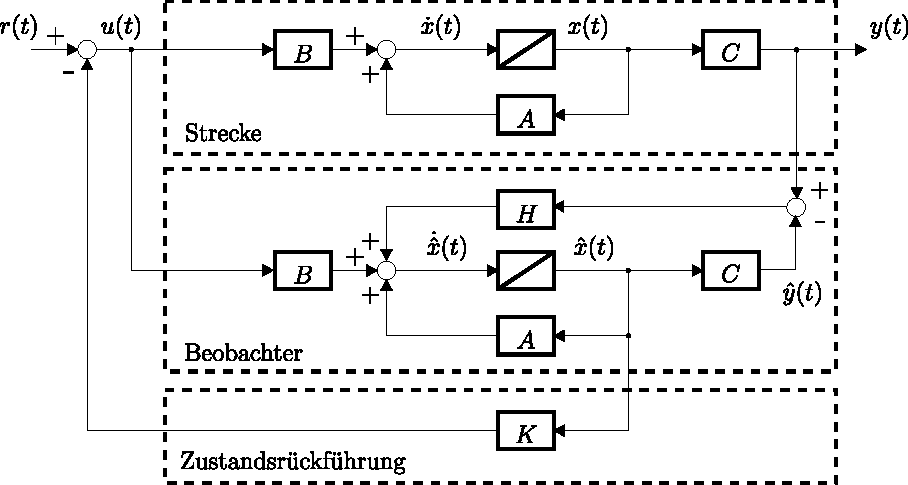
\includegraphics[width=0.85\columnwidth, align=t]{images/beobachter_strecke_beobachter_ZRF.pdf}
\end{center}

Es kann gezeigt werden, dass beide Teilsysteme (Zustandsrückführung und Beobachter) \textbf{separat entworfen} werden können und ein \textbf{stabiles Gesamtsystem} resultiert. \\
Die Bedingungen dafür sind:

\begin{tabular}{ll}
    \tabitem Zustandsrückführung stabil:    & $\det(\lambda_Z \cdot \bm{I} - \bm{A} + \bm{BK}) \overset{!}{=} 0 \quad \rightarrow \forall \lambda_Z \quad \mathrm{Re} \{ \lambda_Z \} < 0$ \\
    \tabitem Beobachter stabil:             & $\det(\lambda_B \cdot \bm{I} - \bm{A} + \bm{HC}) \overset{!}{=} 0 \quad \rightarrow \forall \lambda_B \quad \mathrm{Re} \{ \lambda_B \} < 0$
\end{tabular}

\medskip

Die Eigenwerte (bzw. Pole) des Gesamtsystems entsprechen der \textbf{Vereinigung der Eigenwerte der Teilsysteme}.
Die Eigenwerte (bzw. Pole) könnten auch durch Lösung einer einzigen (aufwendigen) Gleichung gelöst werden:

\vspace{-0.2cm}

$$ \det(\lambda \cdot \bm{I} - \bm{A} + \bm{BK}) \cdot \det(\lambda \cdot \bm{I} - \bm{A} + \bm{HC}) \overset{!}{=} 0 $$

\textbf{Hinweis:} Gezeigt ist die 'Eigenwert-Sicht'. Wenn gezeigt werden soll, dass der Fokus auf den Polen liegt, dann wird in den Gleichungen jeweils $\lambda$ durch $s$ ersetzt.


\subsection{LQG-Verfahren (Linear Quadratic Gaussian Estimation)}

Die duale Methode zum LQR-Verfahren der Zustandsrückführung ist das LQG-Verfahren.
Im Gegensatz zum LQR-Verfahren handelt es sich beim LQG-Verfahren um ein \textbf{stochastisches Optimierungsproblem}.


\subsubsection{Optimale Beobachterverstärkung $\bm{H}$}

Die optimalen Beobachterverstärkungen (als Matrix $\bm{H}$) ergeben sich aus der positiv definiten Lösung der Matrix $\bm{S}$ der entsprechenden Matrix-Ricatti-Gleichung:

\vspace{-0.2cm}

$$ \boxed{ \bm{H} = (\bm{R^{-1} C S})^T = \bm{S C^T R^{-1}} } $$

\textbf{Hinweis:} Meist wird die Lösung $\bm{H}$ direkt mit Matlab ermittelt.


\subsubsection{Eigenschaften des LQG-Verfahrens}

\begin{outline}
    \1 Die Gewichtungsmatritzen $\bm{R}$ und $\bm{Q}$ werden \textbf{positiv definit} gewählt
        \2 Die Gewichtungsmatritzen charakterisieren die Rauschleistung im System
    \1 Ist $\bm{R}$ klein, so ist das Messrauschen gering bzw. die Messung zuverlässig
        \2 Die Verstärkung $\bm{H}$ ist dann grösser und Regelkreis somit schneller
    \1 Die Robustheit des Gesamtsystems ist \textbf{nicht garantiert}, wenn Beobachter und Zustandsrückführung \textbf{unabhängig voneinander} entworfen werden
        \2 Separationsprinzip gilt nicht für Robustheit bei LQG!
\end{outline}


\subsection{Varianten von Beobachtern}{209-211}

\subsubsection{Beobachter für Teilsysteme}

Ein Beobachter kann auch den Ausgang eines Teilsystems (hier $w$) beobachten, statt den Ausgang des Gesamtsystems.
Auch muss der Eingang eines Beobachters nicht der Stellgrösse $u$ entsprechen, sondern kann das Ausgangssignal eines vorherigen Teilsystems sein (hier $w$).

\vspace{-0.2cm}

\begin{center}
    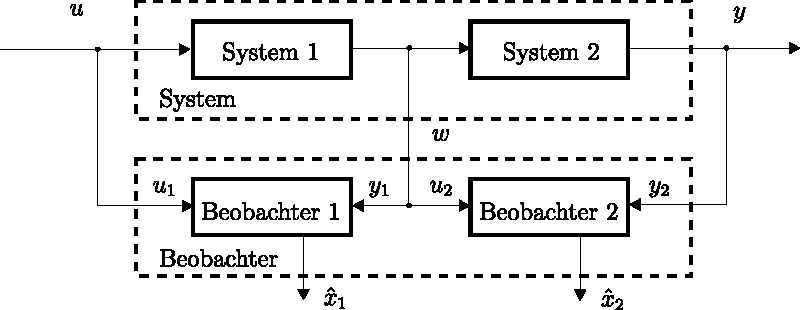
\includegraphics[width=0.8\columnwidth]{images/beobachter_teilsysteme.pdf}
\end{center}

\vspace{-0.2cm}

Durch die Beobachtung von Teilsystemen kann die \textbf{Komplexität beim Entwurf reduziert} werden.


\subsubsection{Redundante Messungen}

Redundante Messungen sind sinnvoll, wenn Messrauschen vorhanden ist.

\smallskip

Zwei Sensoren, welche unabhängig voneinander dieselbe Grösse messen, liefern dasselbe Signal, überlagert von unterschiedlichem Rauschen.
Das Signal kann mit zwei Sensoren besser geschätzt werden, wobei natürlich eine Kosten-Nutzen-Rechnung gemacht werden muss.



\subsubsection{Reduzierter Beobachter}

Wenn Zustandsgrössen rauschfrei gemessen werden können, ist es nicht nötig, diese zu schätzen. 
Es müssen dann nur $n - \mu$ Grössen geschätzt werden. Somit kann der Beobachter reduziert werden.

\smallskip

Bei folgender Darstellung der ZRD des Beobachters wird angenommen, dass die \textbf{Messgrössen einem Teil des Zustandsvektors entsprechen}.
Diese müssen folglich \textbf{nicht} durch den Beobachter geschätzt werden.

\vspace{-0.1cm}

\begin{minipage}[c]{0.5\columnwidth}
    \begin{align*}
        \begin{bmatrix} \dot{x}_{\nu} \\ \dot{x}_{\mu} \end{bmatrix}    &= \begin{bmatrix} \bm{A_{11}}   & \bm{A_{12}} \\ \bm{A_{21}}  & \bm{A_{22}} \end{bmatrix} \cdot \begin{bmatrix} x_{\nu} \\ x_{\mu} \end{bmatrix}
                                                                        + \begin{bmatrix} \bm{B_1} \\ \bm{B_2} \end{bmatrix} \cdot u                                                                                        \\
        y                                                               &= \begin{bmatrix} \bm{0} & \bm{I} \end{bmatrix} \cdot \begin{bmatrix} x_{\nu} \\ x_{\mu} \end{bmatrix}
    \end{align*}
\end{minipage}
\hfill
\begin{minipage}[c]{0.45\columnwidth}
    \begin{tabular}{ll}
        $x_{\mu}$   & gemessene Zustandsgrössen     \\
        $x_{\nu}$   & geschätzte Zustandsgrössen    \\
    \end{tabular}
\end{minipage}

\smallskip

\paragraph{Realisierung des reduzierten Beobachters}

\begin{center}
    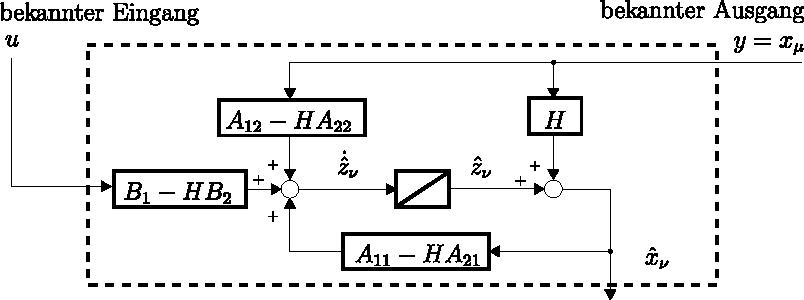
\includegraphics[width=0.8\columnwidth, align=t]{images/beobachter_reduziert.pdf}
\end{center}

\vspace{-0.2cm}


\subsection{Implementierung eines Zustandsreglers mit Beobachter}

Für eine SISO-Strecke wurde ein Zustandsregler mit Beobachter mit Verstärkung $k$ und eine Vorverstärkung $L$ entworfen.

\vspace{-0.2cm}

\begin{center}
    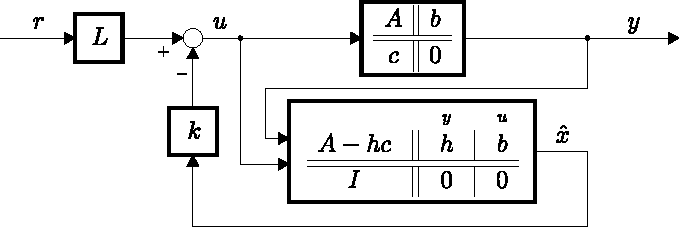
\includegraphics[width=0.8\columnwidth, align=t]{images/beobachter_zustandsregler_vorverstaerkung.pdf}
\end{center}


Das System kann auch so betrachtet werden, dass der Beobachter und die Vorverstärkung mit in den Regler 'gepackt' werden.
Durch einsetzen von $u = L r - k \hat{x}$ (gemäss Regelkreis oben) ergibt sich für das Gesamtregelsystem (unten) die folgende ZV-Darstellung:

\begin{ctabular}{r c c c c c}
    $\dot{\hat{x}} =$   & $(\bm{A}- hc - bk)$   & $\hat{x} \ +$ & $bLr$   & $+ \ hy$  \\
    $u =$               & $-k$                  & $\hat{x} \ +$ & $Lr$    &           \\
\end{ctabular}

\begin{center}
    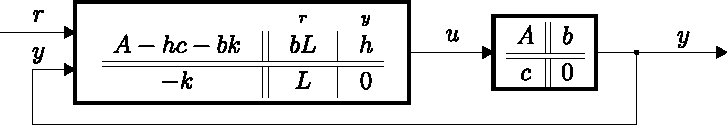
\includegraphics[width=0.8\columnwidth, align=t]{images/beobachter_zustandsregler_gesamtsystem.pdf}
\end{center}

\vspace{-0.2cm}


\subsubsection{Eigenschaften der Implementierung}

\begin{outline}
    \1 Gesamtregler ist MIMO-System mit Eingängen $r$ und $y$
    \1 Die beiden UTF $\frac{U(s)}{R(s)}$ und $\frac{U(s)}{Y(s)}$ haben dieselbe Systemmatrix $(\bm{A} - hc - bk)$
        \2 Beide UTF haben somit \textbf{identische Pole}
        \2 Nullstellen der beiden UTF sind unterschiedlich
\end{outline}

\vspace{-0.4cm}

$$ \frac{U(s)}{R(s)} = \frac{\beta_n s^n \beta_{n-1} s^{n-1} + \cdots + \beta_1 s + \beta_0}{s^n + \alpha_{n-1} s^{n-1} + \cdots + \alpha_1 + \alpha_0} \qquad \quad
    \frac{U(s)}{Y(s)} = \frac{\overline{\beta}_m s^m \overline{\beta}_{m-1} s^{m-1} + \cdots + \overline{\beta}_1 s + \overline{\beta}_0}{s^n + \alpha_{n-1} s^{n-1} + \cdots + \alpha_1 + \alpha_0} $$


\subsubsection{Reglerstruktur -- Zustandsreglers mit Beobachter}

Die folgende Filterform (Direkte Form) implementiert die \textbf{minimale Realisierung} des Reglers mit Beobachter.
Es sind allerdings auch andere Realisierungen möglich.

\vspace{-0.2cm}

\begin{center}
    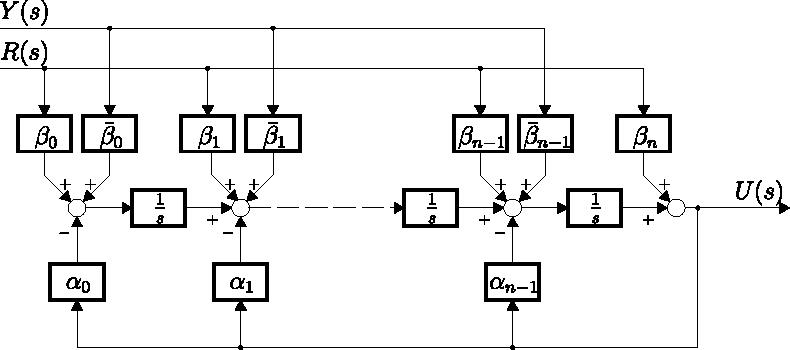
\includegraphics[width=0.8\columnwidth, align=t]{images/beobachter_implementation.pdf}
\end{center}


        \section{Digitale Regelung}

\subsection{Regelkreis mit digitalem Regler}{214}

Ein Regelkreis mit digitalem Regler hat folgende Struktur:

\smallskip

\begin{minipage}[t]{0.64\columnwidth}
    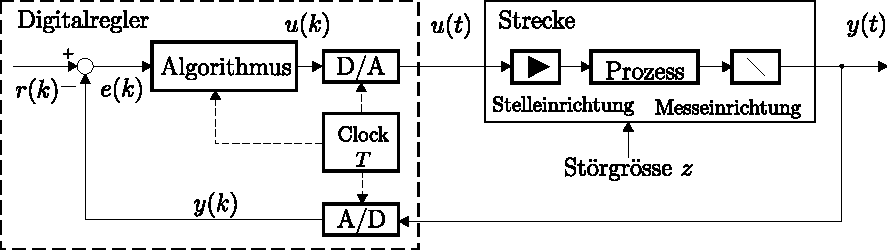
\includegraphics[width=\columnwidth, align=t]{images/dig_reg_regelkreis.pdf}
\end{minipage}
\hfill
\begin{minipage}[t]{0.34\columnwidth}
    \begin{outline}
        \1 Strecke ändert \textbf{nicht}
        \1 Regler arbeitet \textbf{zeitdiskret}
        \1 Zentraler Clock
            \2 Abtastzeit $T$
        \1 Schnittstellen:\\
            A/D bzw. D/A Wandler
    \end{outline}
\end{minipage}


\subsubsection{Vorteile / Nachteile digitale Regler}{215-217}

\begin{itemize}
    \item[+] Struktur / Parameter des Reglers einfach veränderbar \textrightarrow\ adaptive Regelung
    \item[+] Entwicklungsumgebungen (z.B. Simulink) erlauben Simulation des Reglers und anschliessende Code-Generierung
    \item[+] Nichtlineare Regleralgorithmen sind einfach implementierbar 
    \item[+] Digitale Regler können Teil eines hierarchischen Regelsystems sein
    \item[+] Einfacher, schneller Wechsel zwischen verschiedenen Reglern möglich
    \item[+] (Intelligente) Sensoren liefern Daten digital, nicht analog
    \item[-] Wertquantisierung der Signale \textrightarrow\ Quantisierungsrauschen
    \item[-] Zeitquantisierung \textrightarrow\ Totzeit von ca. $50\, \%$ der Abtastzeit $T$ 
    \item[-] Rundungsfehler aufgrund von rechnerischer Zahlendarstellung   
\end{itemize}
%-----------------------------------------------------------------------------------------------------------------------------------
\subsubsection{Diskretisierung eines Integrators}

Kontinuierlich:

\[
G(s)=\frac1s
\]

Rechteck vorwärts:

\[
G(z)=\frac{T}{z-1}
\]

Rechteck rückwärts:

\[
G(z)=\frac{Tz}{z-1}
\]

Trapezregel (Tustin):

\[
G(z)=
\frac{T}{2}
\frac{z+1}{z-1}
\]

\para{Stabilität}

Kontinuierlich:

\[
\Re(\lambda)<0
\]

Diskret:

\[
|z_i|<1
\]

(Pole innerhalb Einheitskreis)
%-----------------------------------------------------------------------------------------------------------------------------------

\subsection{Signale im digitalen Regelkreis}{184}
\label{Signale im digitalen Regelkreis}

Die im Digitalregler verarbeiteten Signale $y(k)$, $r(k)$, $e(k)$ und $u(k)$ sind keine Funktionen der Zeit, sondern \textbf{Folgen von Werten}!

\begin{outline}
    \1 Sensorseitig wird jeweilt zum Zeitpunkt $t = k \cdot T$ das Signal $y(t)$ abgetastet
        \2 \textbf{TP:} Analoges Tiefpassfilter \textrightarrow\ Anti-Aliasing
    \1 Aktorseitig wird mit einem \textbf{ZOH}-Halteglied (Zero-Order-Hold) aus dem diskreten Signal $u(k)$ das Signal $u(t)$ erzeugt, welches während eines Abtastintervalls konstant ist
\end{outline}

\vspace{-0.2cm}

\begin{center}
    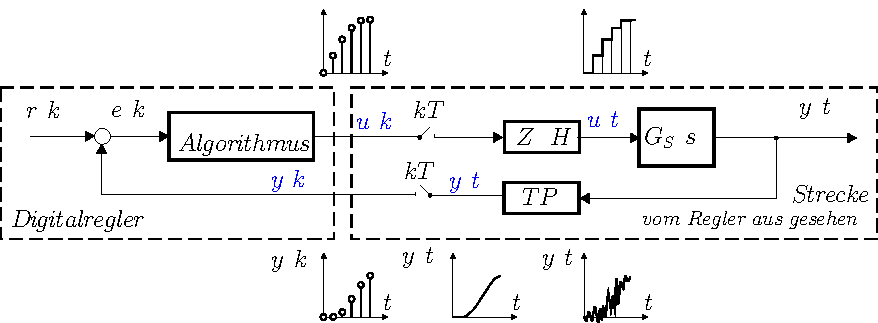
\includegraphics[width=0.9\columnwidth]{images/dig_reg_regelkreis_signale.pdf}
\end{center}

\vspace{-0.2cm}

Damit das Zusammenspiel zwischen digitalem Regler und analoger Strecke korrekt funktioniert, muss die Schnittstelle 'gut funktionieren'.
Da diese Schnittstelle aus A/D- bzw. D/A-Wandlern besteht, müssen die Effekte rund um die \textbf{Signal-Quantisierung} betrachtet werden.


\subsubsection{Quantisierung der Signalwerte / Sättigung}{219-220}

Quantisierung und Sättigung sind \textbf{nichtlineare Effekte}. Es ist daher wichtig, die Auflösung der A/D- und D/A-Wandler geeignet zu wählen.

\smallskip

\begin{outline}
    \1 Zu grobe Quantisierung der Signalwerte führt zu \textbf{Nichtliearität}
    \1 Zu feine Quantisierung der Signalwete hat \textbf{keinen negativen Einfluss} auf Regler
        \2 Ist jedoch teuer
\end{outline}


\subsubsection{Wahl der Abtastzeit $\bm{T}$}{220-221}

Im Prinzip gilt: \textbf{Je kleiner die Abtastzeit $\bm{T}$ eines Reglers ist, desto besser kann der Regler arbeiten}.

\smallskip

\begin{outline}
    \1 Wird die Abtastzeit zu klein gewählt, können numerische Probleme entstehen
    \1 Wird die Abtastzeit zu gross gewählt, kommt es zu Überschwingen oder bis zur Destabilisierung des Systems
\end{outline}

\smallskip

Damit die Abtastzeit $T$ des Reglers entsprechend gewählt werden kann, gibt es 'Faustregeln', bei welchen die Führungsgrösse, der offene Regelkreis 
(Regelstrecke) oder der geschlossene Regelkreis betrachtet wird.

\medskip

\paragraph{Faustregel: Abtastzeit mittels Führungsgrösse}

Das Spektrum der Führungsgrösse $r(t)$ ist begrenzt durch $\omega_r$. Damit bei der Abtastung von $y(t)$ keine Informationen verloren gehen,
wird das Nyquist-Theorem meist um \cbl{Faktor 10} übererfüllt.

\vspace{-0.2cm}

$$ \omega_s = \frac{2 \pi}{T} \leq \cbl{10} \cdot 2 \, \omega_r $$


\columnbreak


\paragraph{Faustregel: Abtastzeit mittels Regelstrecke}

\begin{minipage}[c]{0.45\columnwidth}
    Aus der \textbf{Schrittantwort der Regelstrecke} werden mittels \textbf{Wendetangente} die folgenden Parameter herausgelesen und damit die Abtastzeit bestimmt. 

    \smallskip

    \textrightarrow\ Wenn sich die verschiedenen \textbf{Empfehlungen widersprechen}, ist tendenziell der \textbf{kleinere Wert} als Abtastzeit $T$ zu wählen!
\end{minipage}
\hfill
\begin{minipage}[c]{0.53\columnwidth}   
    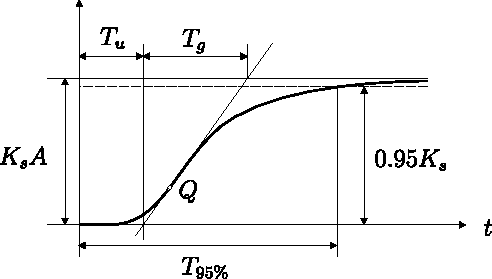
\includegraphics[width=\columnwidth, align=t]{images/dig_reg_schrittantwort_wendetangente.pdf}
\end{minipage}

\vspace{-0.1cm}

\begin{ctabular}{lll}
    \toprule
    \textbf{Kennwert}   & \textbf{Abtastzeit}                                   & \textbf{Kommentar}                \\
    \midrule
    $T_u$               & $0.1 \cdot T_u \leq T \leq 0.25 \cdot T_u$            & Prozess mit ausgeprägter Totzeit  \\
    \midrule
    $T_g$               & $T \leq 0.1 \cdot T_g$                                & $T_g \gg T_u$                     \\
    \midrule
    $T_{95\%}$          & $0.05 \cdot T_{95\%} \leq T \leq 0.1 \cdot T_{95\%}$  &                                   \\
    \bottomrule
\end{ctabular}

\smallskip


\paragraph{Faustregel: Abtastzeit mittels geschlossenem Regelkreis}

\textbf{Voraussetzung:} Es existiert bereits ein Regler in Analogtechnik oder in der Simulation.

\smallskip

\begin{minipage}[t]{0.45\columnwidth}
    Aus der \textbf{Schrittantwort des geschlossenen Regelkreises} werden die folgenden Parameter herausgelesen und damit die Abtastzeit bestimmt.

    \smallskip

    \textrightarrow\ Wenn sich die verschiedenen \textbf{Empfehlungen widersprechen}, ist tendenziell der \textbf{kleinere Wert} als Abtastzeit $T$ zu wählen!
\end{minipage}
\hfill
\begin{minipage}[t]{0.53\columnwidth}   
    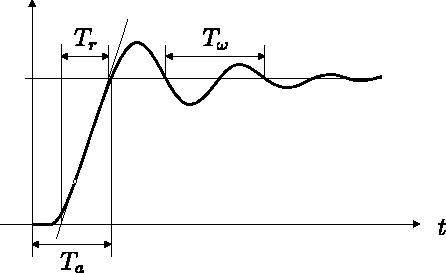
\includegraphics[width=\columnwidth, align=t]{images/dig_reg_schrittantwort_kennwerte.pdf}
\end{minipage}

\vspace{-0.1cm}

\begin{ctabular}{ll}
    \toprule
    \textbf{Kennwert}   & \textbf{Abtastzeit}                           \\
    \midrule
    $T_a$               & $0.05 \cdot T_a \leq T \leq 0.1 \cdot T_a$    \\
    \midrule
    $T_r$               & $0.05 \cdot T_r \leq T \leq 0.1 \cdot T_r$    \\
    \midrule
    $T_{\omega}$        & $T \leq 0.05 \cdot T_{\omega}$                \\
    \bottomrule
\end{ctabular}



\subsubsection{Anti-Aliasing Filter}{222-223}

Ein Signal $y(t)$ wird periodisch mit Abtastzeit $T$, bzw. mit Abtastfrequenz $\omega_s$ abgetastet. 
Die Folge der abgetasteten Werte ist dann $y(k)$.

\vspace{-0.5cm}

$$ y(t) = A \cdot \cos(\omega_0 t) \quad \underrightarrow{\text{sampling: } \omega_s} \quad y(kT) = A \cdot \cos(\omega_0 \cdot kT) \qquad \text{mit } \omega_s = 2 \pi f_s = \frac{2 \pi}{T} $$

\vspace{-0.2cm}

Dieselbe Folge resultiert aber auch, wenn ein Signal $\tilde{y}(t) = A \cdot \cos\left([n \cdot \omega_s \pm \omega_0] \cdot t \right)$ mit $\omega_s$ abgetastet wird ($n$ ganzzahlig). \\
Hat solch ein Signal $\tilde{y}(t)$ Frequenzanteile, die \textbf{oberhalb der Nyquistfrequenz $\bm{\omega_N}$} liegen, so werden diese
Anteile ebenfalls ins Frequenzband $\omega = [0, \, \omega_N]$ abgebildet. 

\smallskip

Frequenzanteile, welche oberhalb der Nyquistfrequenz $\omega_N$ liegen, müssen deshalb mit einem \textbf{Anti-Aliasing-Filter (Tiefpass)} herausgefiltert werden.
Somit ist das Nyquist-Kriterium erfüllt.

\vspace{-0.2cm}

$$ \omega_N = \frac{\omega_s}{2} = \frac{\pi}{T} \quad \Leftrightarrow\ \quad \omega_s > 2 \cdot \omega_{\rm Signal} $$


\subsection{Reglerentwurf -- direkt vs. indirekt}{224-225}

\begin{minipage}[t]{0.48\columnwidth}
    \raggedright
    \begin{outline}
        \1  Indirekter digitaler Reglerentwurf
            \2 $G_S(s)$ \textrightarrow\ 'links herum' \textrightarrow\ $G_{R,I}(z)$
            \2 Zeitkontinuerlicher Regler wird zeitdiskret approximiert
    \end{outline}
\end{minipage}
\hfill
\begin{minipage}[t]{0.48\columnwidth}
    \raggedright
    \begin{outline}
        \1 Direkter digitaler Reglerentwurf
            \2 $G_S(s)$ \textrightarrow\ 'rechts herum' \textrightarrow\ $G_{R,D}(z)$
            \2 'Digitale Natur' des Reglers von Anfang an berücksichtigt
    \end{outline}
\end{minipage}


\begin{center}
    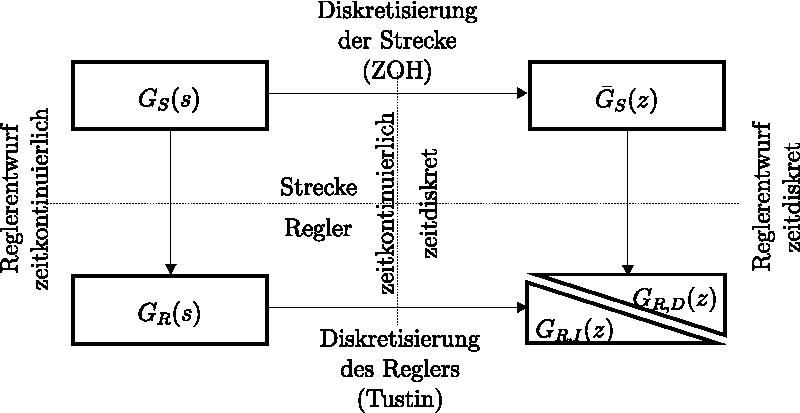
\includegraphics[width=0.8\columnwidth, align=t]{images/dig_reg_reglerentwurf.pdf}
\end{center}

% \begin{minipage}[t]{0.51\columnwidth}
%     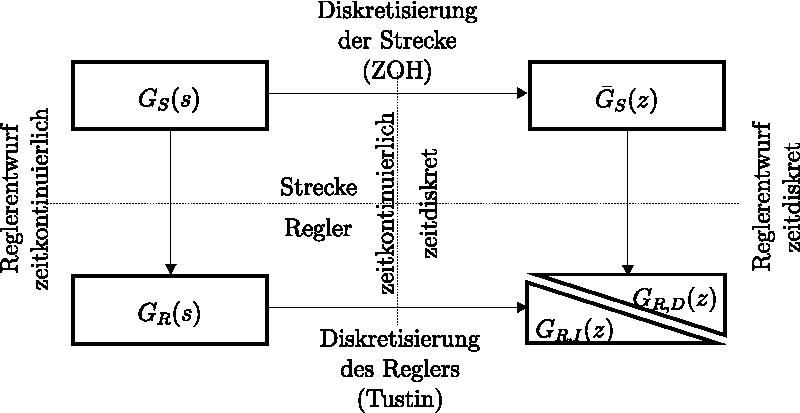
\includegraphics[width=\columnwidth, align=t]{images/dig_reg_reglerentwurf.pdf}
% \end{minipage}
% \hfill
% \begin{minipage}[t]{0.48\columnwidth}
%     \raggedright
%     \begin{outline}
%         \1  \textbf{Indirekter digitaler Reglerentwurf}
%             \2 $G_S(s)$ \textrightarrow\ 'links herum' \textrightarrow\ $G_{R,I}(z)$
%             \2 Zeitkontinuerlicher Regler wird zeitdiskret approximiert
%         \1 Direkter digitaler Reglerentwurf
%             \2 $G_S(s)$ \textrightarrow\ 'rechts herum' \textrightarrow\ $G_{R,D}(z)$
%             \2 'Digitale Natur' des Reglers von Anfang an berücksichtigt
%     \end{outline}
% \end{minipage}


        
\section{Indirekter digitaler Reglerentwurf}

\subsection{Approximationen für Diskretisierung}{226}

\begin{minipage}[c]{0.48\columnwidth}
    Ein kontinuierlicher Regler (hier I-Regler) weist folgendes Verhalten auf:
\end{minipage}
\hfill
\begin{minipage}[c]{0.48\columnwidth}
    $$ u(t) = K_R \cdot \int\limits_0^t e(\tau) \, \diff \tau $$
\end{minipage}


Der entsprechende zeitdiskrete Regler kann \textbf{nicht exakt} gebildet werden, da $e(t)$ nur zu diskreten Zeitpunkten $e(kT)$ bekannt ist.
Geht man davon aus, dass $e(t)$ \textbf{nicht start ändert} (\textrightarrow\ geeignete Wahl der Abtastzeit $T$), dann kann $u(k)$
folgendermassen approximiert werden:

\vspace{-0.2cm}

$$ u(k) = K_R \cdot \int\limits_0^{kT} e(\tau) \, \diff \tau
    = \underbrace{K_R \cdot \int\limits_0^{kT- T} e(\tau) \, \diff \tau}_{u(k-1)} 
    + \underbrace{K_R \cdot \int\limits_{kT-T}^{kT} e(\tau) \, \diff \tau}_{\approx A} $$


\subsubsection{Approximationen der Fläche $\bm{A}$}

Die Fläche $A$ kann auf mehrere Arten approximiert werden:


\begin{minipage}[c]{0.35\columnwidth}
    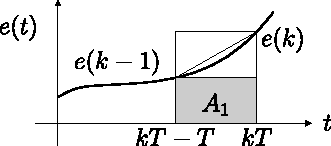
\includegraphics[width=\columnwidth, align=t]{images/dig_reg_approximation_integration.pdf}
\end{minipage}
\hfill
\begin{minipage}[c]{0.64\columnwidth}
    \resizebox{\columnwidth}{!}
    {
        \renewcommand{\arraystretch}{1.3}
        \begin{tabular}{ll@{}}
            Rechteckregel vorwärts (Euler)      & $A = T \cdot e(k-1)$                      \\
            Rechteckregel rückwärts             & $A = T \cdot e(k)$                        \\
            \textbf{Trapezregel (Tustin)}       & $A = T \cdot \dfrac{e(k-1) + e(k)}{2} $ 
        \end{tabular}
        \renewcommand{\arraystretch}{1}
    }
\end{minipage}

\vspace{0.2cm}
\textbf{Hinweis:} Für die Diskretisierung von Reglern wird die \textbf{Trapez-Approximation} verwendet, da diese am genausten ist.


\subsection{Vorgehen: Diskretisierung eines Reglers}{226-228}

Die Ordnung des Reglers bleibt bei der Diskretisierung erhalten.

$$ G_R(s) = \frac{U(s)}{E(s)} = \frac{b_m s^m + b_{m-1} s^{m-1} + \ldots + b_1 s + b_0}{s^n + a_{n-1} s^{n-1} + \ldots + a_1 s + a_0} \quad (m \leq n) $$
$$ \overline{G}_R(z) = \frac{U(z)}{E(z)} = \frac{\overline{b}_m z^m + \overline{b}_{m-1} z^{m-1} + \ldots + \overline{b}_1 z + \overline{b}_0}{z^n + \overline{a}_{n-1} z^{n-1} + \ldots + \overline{a}_1 z + \overline{a}_0} $$

\begin{enumerate}
    \item UTF des Reglers $G_R(s)$ bestimmen
    \item Wahl der Abtastzeit $T$ und Diskretisierungsmethode \textrightarrow\ typischerweise \textbf{Tustin}
    \item Transformation zu $\overline{G}_R(z)$  durch Substitution aller Variablen $s$ in $G_R(s)$ mit gewünschter Approximation \textrightarrow\ siehe Abschnitt \ref{Approximationsmethoden -- Substitutionsterme}
    \item Falls nötig: Doppelbrüche in $\overline{G}_R(z)$ eliminieren und $T$ numerisch einsetzen
    \item $\overline{G}_R(z)$ 'separieren' und ausmultiplizieren \\
        $\overline{b}_m z^m \cdot E(z) + \ldots + \overline{b}_1 z \cdot E(z) + \overline{b}_0 \cdot E(z) = z^n \cdot U(z) + \ldots + \overline{a}_1 z \cdot U(z) + \overline{a}_0 \cdot U(z)$
    \item Umformen in Differenzengleichung \\
        $\overline{b}_m \cdot e(k+m)  + \ldots + \overline{b}_1 \cdot e(k+1) + \overline{b}_0 \cdot e(k) = u(k+n) + \ldots + \overline{a}_1 \cdot u(k+1) + \overline{a}_0 \cdot u(k)$
    \item Resultierende zeitinvariante Gleichung $u(k)$ auflösen und bei Bedarf um $n$ Zeitschritte verschieben
\end{enumerate}



\subsubsection{Substitutionsterme z-Transformation}{227}
\label{Approximationsmethoden -- Substitutionsterme}

\begin{ctabular}{lcc}
    \toprule
    \textbf{Methode}                & \textbf{Substitution von} $\bm{s}$                & \textbf{Substitution von} $\bm{z}$    \\
    \midrule
    Rechteckregel vorwärts (Euler)  & $s = \frac{z - 1}{T}$                             & $z = 1 + sT$                          \\
    \midrule
    Rechteckregel rückwärts         & $s = \frac{1}{T} \cdot \frac{z - 1}{z}$           & $z = \frac{1}{1 - sT}$                \\
    \midrule
    \textbf{Tustin}                 & $\bm{s = \frac{2}{T} \cdot \frac{z - 1}{z + 1}}$  & $z = \frac{2 + sT}{2 - sT}$           \\
    \bottomrule
\end{ctabular}


% \begin{center}
%     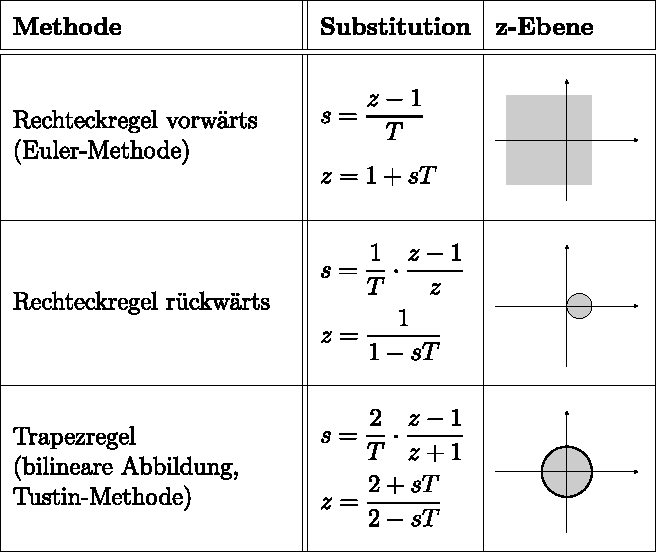
\includegraphics[width=0.8\columnwidth, align=t]{images/dig_reg_substitution_z_trafo.pdf}
% \end{center}


\example{Lead-Regler diskretisieren}

Gegeben sei die Übertragungsfunktion $G_R(s)$ eines \textbf{kontinuierlichen} Reglers.
Daraus soll die zu implementierende \textbf{Differenzengleichung} ermittelt werden. 

\vspace{-0.2cm}

\begin{ctabular}{lcl}
    \tabitem Diskretisierungsmethode: \textbf{Tustin}   &   & \tabitem Abtastzeit: $T = 0.1 \, \second$
\end{ctabular}

\vspace{-0.3cm}

$$ \bm{1.} \quad G_R(s) = 4 \cdot \frac{s+1}{s+5} \quad {\textrightarrow\ } \bm{2.} $$
$$ \overline{G}_{R}(z) \overset{\bm{3.}}{=} 4 \cdot \frac{1 + \frac{2}{T} \frac{z-1}{z+1}}{5 + \frac{2}{T} \frac{z-1}{z+1}} 
    \overset{\bm{4.}}{=} 4 \cdot \frac{T (z+1) + 2 (z-1)}{5 T (z+1) + 2 (z-1)} = \frac{3.36 z - 3.04}{z - 0.6} = \frac{U(z)}{E(z)} $$
$$ \bm{5.} \quad z \cdot U(z) - 0.6 \cdot U(z) = 3.36 z \cdot E(z) - 3.04 \cdot E(z) $$
$$ \bm{6.} \quad u(k+1) - 0.6 \cdot u(k) = 3.36 \cdot e(k+1) - 3.04 \cdot e(k) \qquad \big| \text{-1 Zeitschritt} $$
$$ \bm{7.} \quad u(k) = 0.6 \cdot u(k-1) + 3.36 \cdot e(k) - 3.04 \cdot e(k-1) $$


\subsection{Empirische Einstellregeln für digitale PID-Regler}

Für eine Strecke mit Totzeit $G_S(s)$ wird ein \textbf{zeitkontinuierlicher} PID-Regler mit UTF $G_R(s)$ entworfen.
Dieser kann mit den empirischen Einstellregeln von Ziegler-Nichols parametrisiert werden.

\vspace{-0.2cm}

$$ 
    G_S(s) = \frac{K_S}{s T_g + 1} \cdot e^{- s T_u} \qquad \qquad
    G_R(s) = K_R \left( 1 + \frac{1}{s T_N} + s T_V \right)
$$

Wird der \textbf{PID-Regler diskretisiert}, so kann er nach den Regeln von \textbf{Takahashi, Chan und Auslander} empirisch eingestellt werden (siehe Abschnitt \ref{Einstellregeln nach Takahashi, Chan und Auslander}).


\subsubsection{Einstellregeln nach Takahashi, Chan und Auslander}{230}
\label{Einstellregeln nach Takahashi, Chan und Auslander}

\textbf{Voraussetzung: } $\bm{T \leq 2 T_u}$

\begin{ctabular}{l c c c}
    \toprule
    \textbf{Regler}     & $\bm{K_R}$                                        & $\bm{T_N}$                                & $\bm{T_V}$                    \\
    \midrule
    P-Regler            & $\frac{T_g}{K_S (T_u + T)}$                       & $-$                                       & $-$                           \\
    \midrule
    PI-Regler           & $0.9 \cdot \frac{T_g}{K_S (T_u + \frac{T}{2})}$   & $3.33 \left( T_u + \frac{T}{2} \right)$   & $-$                           \\
    \midrule
    PID-Regler          & $1.2 \cdot \frac{T_g}{K_S (T_u + T)}$             & $ \left( T_u + \frac{T}{2} \right)$       & $0.5 \left( T_u + T \right)$  \\
    \bottomrule
\end{ctabular}

\textbf{Hinweis:} Für eine Abtastzeit von $T=0$ entspricht obige Tabelle der zeitkontinuerlichen Ziegler-Nichols Approximation.


        
\section{z-Transformation / Zeitdiskrete Übertragungsfunktion}

\subsection{Folgen (und deren z-Transformation)}{230}

Eine zeitliche Folge $f(k)$ bricht typischerweise nicht ab und wird folgendermassen beschrieben:

\vspace{-0.2cm}

$$ f(k) = \{1, \, a, \, a^2, \, a^3, \, \ldots \} = a^k \qquad \text{für } k \geq 0 \quad k \text{ ganzzahlig} $$


\subsubsection{Spezielle Folgen: Abbrechende Folgen}

Bei einer abbrechenden Folge liegen \textbf{alle Pole bei Null}. \\
Man spricht in diesem Fall von einem \textbf{FIR-Filter} (Finite Response Filter)


\example{Abbrechende Folge und deren z-Transformierte}

\vspace{-0.2cm}

$$ f(k) = \left\{ f(0), \, f(1), \, f(2), \, f(3), \, 0, \, 0, \, 0, \, \ldots  \right\} $$

\vspace{-0.2cm}

$$ F(z) = f(0) + \frac{f(1)}{z} + \frac{f(2)}{z^2} + \frac{f(3)}{z^3} = \frac{f(0) \, z^3 + f(1) \, z^2 + f(2) \, z + f(3)}{z^3}$$



\subsection{z-Transformation -- Definition}{232}

Die Überführung eine Folge in den Frequenzbereich erfolgt mittels z-Tranaformation und ist definiert als

\vspace{-0.2cm}

$$ \boxed{ F(z) = \mathcal{Z}\{f(k)\} = \sum\limits_{k=0}^{\infty} f(k) \cdot z^{-k} \quad \text{mit der komplexen Variablen } z } $$


\textrightarrow\ Häufig werden \textbf{Tabellen} und die \textbf{Eigenschaften} der z-Transformation verwendet \\
\textrightarrow\ Siehe \ref{zTransformierte einger Funktionen} und \ref{Eigenschaften der z-Transformation}



\subsection{z-Transformierte einiger Funktionen}{232}
\label{zTransformierte einger Funktionen}

Alle Folgen $f(k)$ sind nur für für $k \geq 0$ und ganzzahlige $k$ definiert.

\smallskip

\begin{minipage}[t]{0.44\columnwidth}
    \begin{center}
        \renewcommand{\arraystretch}{1.4}
        \begin{tabular}{c c c}
            \toprule
            $\bm{f(k)}$                             & $\laplace$    & $\bm{F(z)}$                                       \\
            \midrule
            $\delta(k)$                             & $\laplace$    & $1$                                               \\
            \midrule
            $\varepsilon(k)$                        & $\laplace$    & $\frac{z}{z-1}$                                   \\
            \midrule
            $k$                                     & $\laplace$    & $\frac{z}{(z-1)^2}$                               \\
            \midrule            
            $k^2$                                   & $\laplace$    & $\frac{z(z+1)}{(z-1)^3}$                          \\
            \midrule
            $a^k$                                   & $\laplace$    & $\frac{z}{z-a}$                                   \\
            \bottomrule
        \end{tabular}
        \renewcommand{\arraystretch}{1}
    \end{center}
\end{minipage}
\hfill
\begin{minipage}[t]{0.54\columnwidth}
    \begin{center}
        \renewcommand{\arraystretch}{1.4}
        \begin{tabular}{c c c}
            \toprule
            $\bm{f(k)}$                             & $\laplace$    & $\bm{F(z)}$                                           \\
            \midrule
            $\cos(bk)$                              & $\laplace$    & $\frac{z(z - \cos(b))}{z^2 - 2z \cos(b) + 1}$         \\
            \midrule
            $\sin(bk)$                              & $\laplace$    & $\frac{z \sin(b)}{z^2 - 2z \cos(b) + 1}$              \\
            \midrule
            $k \cdot a^k$                           & $\laplace$    & $\frac{az}{(z-a)^2}$                                  \\
            \midrule
            $k \cdot \cos(bk)$                      & $\laplace$    & $\frac{z(z - a \,\cos(b))}{z^2 - 2az \cos(b) + a^2}$  \\
            \midrule
            $k \cdot \sin(bk)$                      & $\laplace$    & $\frac{z a \sin(b)}{z^2 - 2az \cos(b) + a^2}$         \\
            \bottomrule
        \end{tabular}
        \renewcommand{\arraystretch}{1}
    \end{center}
\end{minipage}

\smallskip

\textbf{Hinweis:} $\varepsilon(k)$ ist eine Folge von $1$ern \\
\textbf{Hinweis:} Oft wird $\frac{F(z)}{z}$ in der Tabelle gefunden

\para{DC-Verstärkung}

\[
G_{DC}
=
G(z)\Big|_{z=1}
\]

\subsection{Eigenschaften der z-Transformation}{235}
\label{Eigenschaften der z-Transformation}

\resizebox{\columnwidth}{!}{
    \begin{tabular}{ccc}
        \toprule
        \textbf{Zeitbereich}                                                        & \textbf{Bildbereich}                          & \textbf{Operation im Zeitbereich}     \\
        \midrule
        $a_1 f_1(k) + a_2 f_2(k)$                                                   & $a_1 F_1(z) + a_2 F_2(z)$                     & Superposition                         \\
        \midrule
        $f(k+1)$                                                                    & $z F(z) - z \, f(0)$                          & Linksverschiebung...                  \\
        \midrule
        $f(k+2)$                                                                    & $z^2 F(z) - z^2 f(0) - z f(1)$          & ...mehrfach angewendet                \\
        \midrule
        $f(k-m) \quad m \geq 0$                                                     & $\frac{1}{z^m} F(z)$                          & Rechtsverschiebung                    \\
        \midrule
        $\sum\limits_{\nu=0}^k f(\nu)$                                              & $\frac{z}{z-1} F(z)$                          & Partialsummen                         \\
        \midrule
        $\sum\limits_{\nu=0}^k f_1(\nu) \cdot f_2(k - \nu)$                         & $F_1(z) \cdot F_2(z)$                         & Faltung                               \\
        \bottomrule
    \end{tabular}
}


\subsubsection{Grenzwertsätze der z-Transformation}{235}

\textbf{Achtung:} Grenzwertsätze dürfen nur angewendet werden, wenn Grenzwerte existieren! \\
\textrightarrow\ In der Regelungstechnik eigentlich immer gegeben...

\begin{center}
    \begin{tabular}{l c ll}
        \toprule
        \textbf{Zeitbereich}                &       & \textbf{Bildbereich}                                      & \textbf{Bezeichnung}      \\
        \midrule
        $f(0)$                              & $=$   & $\lim\limits_{z \to \infty} F(z)$                         & Anfangswerttheorem        \\
        \midrule
        $\lim\limits_{k \to \infty} f(k)$   & $=$   & $\lim\limits_{z \to 1} \left[ (z-1) \cdot F(z) \right]$   & Endwerttheorem            \\
        \bottomrule
    \end{tabular}
\end{center}


\subsection{Rücktransformation}
\label{Rücktransformation}

Die Rücktransformation kann auf mehrere Arten erreicht werden:

\smallskip

\begin{enumerate}
    \item Direktes benutzen von Tabellen in Rückwärtsrichtung
    \item Zerlegung von $F(z)$ in einfachere, tabellierte Ausdrücke \textrightarrow\ Partialbruchzerlegung
    \item Polynomdivision bzw. Reihenentwicklung von $f(z)$ in negativen Potenzen von $z$
    \item (Allgemeine Umkehroperation zur Definition der z-Transformation)
\end{enumerate}

\smallskip 

\textbf{Bemerkung zu 2.:} Statt $F(z)$ zu zerlegen wird der Ausdruck $\frac{F(z)}{z} = s_1 + s_2 + \ldots$ zerlegt.
Anschliessend werden die Ausdrücke $z \cdot s_i$ rücktransformiert, deren Summe $f(k)$ ergibt. \\
Somit ist die Wahrscheinlicheit höher, den benötigten Term in der Tabelle zu finden. 



\subsection{Beispiele zur z-Transformation}

\example{Geometrische Folge im Frequenzbereich}

Die geometrische Folge ist das Pendant zur zeitkontinuierlichen Exponentialfunktion.

\vspace{-0.2cm}

\[
    F(z)    = \sum\limits_{k=0}^{\infty} a^k \cdot z^{-k} = \sum\limits_{k=0}^{\infty} a^k \cdot \left( \frac{a}{z} \right)^k
            = 1 + \frac{a}{z} + \left( \frac{a}{z} \right)^2 + \left( \frac{a}{z} \right)^3 + \ldots 
\]

Durch eine geeignete Umformung kann die Folge anders dargestellt werden und anschliessend nach $F(z)$ aufgelöst werden.

\vspace{-0.2cm}

\[
    F(z) - 1 = \frac{a}{z} \cdot F(z) \quad \Leftrightarrow \quad 
    1 = F(z) \left( 1 - \frac{a}{z} \right) \quad \Leftrightarrow \quad 
    F(z) = \frac{z}{z-a}
\]


\example{Periodische Folge}

\vspace{-0.2cm}

$$ f_5(k) = \{ \underbrace{0, \, 0, \, 0, \, 0, \,}_{n \text{ Glieder}} \underbrace{ h(0), \, h(1), \, \ldots, \, h(m-1)}_{m \text{ Glieder}}, \underbrace{ h(0), \, h(1), \, \ldots, \, h(m-1)}_{m \text{ Glieder}}, \, \ldots \} $$

$$ F_5(z) = z^{-m} \cdot F_5(z) + z^{-n} \cdot H(z)  \qquad \Rightarrow\ \qquad F_5(z) = \frac{1}{z^n} \frac{z^m}{z^m -1} H(z) $$


\textrightarrow\ $H(z)$ entspricht der z-Transformierten von $\left\{  h(0), \, h(1), \, \ldots, \, h(m-1) 
, \, 0, \, 0, \, \ldots \right\}$


\example{Ausgangssignal bestimmen}

Der Ausgang entspricht der \textbf{Faltung} vom Eingangssignal und Impulsantwort: 
$$ y(k) = u(k) * g(k) $$
Bei jedem Schritt $k$ wird die Impulsantwort mit dem aktuellen $u(k)$ 'skaliert' um $k$ Schritte nach rechts geschoben.

\smallskip

Für $u(k) = \{ 1, \, 0, \, 1, \, 0 , \, 0, \, \ldots \}$ und $g(k) = \{ 6, \, -2, \, -2, \, -2 , \, 0, \, 0, \, \ldots \}$ soll das Ausgangssignal $y(k)$ berechnet werden.

\begin{ctabular}{r l c c c c c c c}
    $u(0) \cdot g(k) =$     & $\{ 6,$   & $-2,$ & $-2,$ & $-2,$ & $0,$  & $0,$  & $0,$  & $\ldots \}$   \\
    $u(1) \cdot g(k-1) =$   & $\{ 0,$   & $0,$  & $0,$  & $0,$  & $0,$  & $0,$  & $0,$  & $\ldots \}$   \\
    $u(2) \cdot g(k-2) =$   & $\{ 0,$   & $0,$  & $6,$  & $-2,$ & $-2,$ & $-2,$ & $0,$  & $\ldots \}$   \\
    $y(k) =$                & $\{ 6,$   & $-2,$ & $4,$  & $-4,$ & $-2,$ & $-2,$ & $0,$  & $\ldots \}$   \\
\end{ctabular}



\example{Lösen einer linearen Differenzengleichung im Bildbereich}

Wie eine Differentialgleichung mittels Laplace-Transformation wird auch eine Differenzengleichung mittels z-Transformation in drei Schritten gelöst:

\smallskip

\begin{enumerate}
    \item Überführung der Differenzengleichung (DG) in den Bildbereich (\textrightarrow\ z-Transformation)
    \item Lösen des resultierenden algebraischen Ausdrucks
    \item Rücktransformation von $Y(z)$ in den Zeitbereich (\textrightarrow\ siehe Abschnitt \ref{Rücktransformation})
\end{enumerate}


$$ \text{Differenzengleichung:} \qquad  a_1 \cdot y(k+1) + a_0 \cdot y(k) = b_0 \cdot u(k) $$

\vspace{-0.2cm}

$$ \bm{1.} \quad a_1 \cdot z \cdot Y(z) - a_1 \cdot z \cdot y(0) + a_0 \cdot Y(z) = b_0 \cdot U(z) $$
$$ \bm{2.} \quad Y(z) = \frac{b_0}{a_0 + a_1 \cdot z} \cdot U(z) + \frac{z}{a_0 + a_1 \cdot z} \cdot y(0) \quad \underrightarrow{\bm{3.} \text{ Tabellen}} \quad y(z) $$ 


\subsection{Zeitdiskrete Übertragungsfunktion}{238-239}

Die \textbf{zeitdiskrete Übertragungsfunktion} $\bm{G(z)}$ beschreibt das Verhalten zwischen Ausgang und Eingang eines diskreten 
Systems und ergibt sich aus der Differenzengleichung im Zeitbereich.

\vspace{-0.4cm}

$$ G(z) = \frac{Y(z)}{U(z)} = \frac{b_m z^m + b_{m-1} z^{m-1} + \ldots + b_0}{z^n + a_{n-1} z^{n-1} + \ldots + a_0} = K \cdot \frac{(z - z_1) (z - z_2) \ldots (z - z_m)}{(z - p_1) (z - p_2) \ldots (z - p_n)} \quad (m \leq n)$$

\textbf{Hinweis:} Für $m > n$ wäre $G(z)$ \textbf{akausal} und somit nicht realisierbar

\smallskip

\textrightarrow\ Gerechnet werden kann mit $G(z)$ gleich wie mit $G(s)$


\subsubsection{DC-Gain}

Der DC-Gain ist leicht anders definiert als bei der Laplace-Transformation

\smallskip

\begin{minipage}[t]{0.48\columnwidth}
    \paragraph{z-Transformation}

    \vspace{-0.2cm}

    $$ \text{DC-Gain} = G(z) \Big|_{z=1} $$
\end{minipage}
\hfill
\begin{minipage}[t]{0.48\columnwidth}
    \paragraph{Laplace-Transformation}

    \vspace{-0.2cm}

    $$ \text{DC-Gain} = G(s) \Big|_{s=0} $$
\end{minipage}



\subsection{Stabilität einer zeitdiskreten Übertragungsfunktion}{240-241}

Für die Untersuchung der Stabilität eines Systems wird der \textbf{Nenner $\bm{N(z)}$ der Übertragungsfunktion} $\bm{G(z)}$ betrachtet.

\smallskip

% SigSys2 mit Anpassungen
Für \textbf{Grenzstabilität} gilt eine \textbf{UND-Verknüpfung} der aufgeführten Punkte. \\
Für \textbf{Stabilität und Instabilität} gilt eine \textbf{ODER-Verknüpfung} der aufgeführten Punkte.

\vspace{0.1cm}

\begin{outline}
    \1 \textbf{Stabil:} 
        \2 Alle Polstellen innerhalb des Einheitskreises \textrightarrow\ $\abs{z} < 1$
        \2 Keine Polstellen vorhanden 
    \1 \textbf{Asymptotisch stabil:}
        \2 Alle Polstellen innerhalb des Einheitskreises \textrightarrow\ $\abs{z} < 1$
    \1 \textbf{Grenzstabil:} 
        \2 \textbf{Keine} Polstellen ausserhalb des Einheitskreises \textrightarrow\ $\abs{z} > 1$
        \2 Mindestens eine \textbf{einfache Polstelle} auf dem Einheitskreis \textrightarrow\ $\abs{z} = 1$
        \2 \textbf{Keine doppelten} Polstellen auf dem Einheitskreis \textrightarrow\ $\abs{z} = 1$
    \1 \textbf{Instabil:} 
        \2 Mindestens eine Polstelle ausserhalb des Einheitskreises \textrightarrow\ $\abs{z} > 1$
        \2 Mindestens eine \textbf{mehrfache Polstelle} auf dem Einheitskreis \textrightarrow\ $\abs{z} = 1$
\end{outline}

\smallskip

\textbf{Hinweis:} 'Stabil' ist ein Synonym für 'asymptotisch stabil' \\
\textbf{Hinweis:} Tustin erhält die Stabilitätseigenschaften eines Systems



\subsubsection{Jury-Kriterium}{241}

Als Pendant zum Routh-Kriterium im Laplace-Bereich existiert in der z-Ebene das Jury-Kriterium.
Somit kann vereinfacht festgestellt werden, ob sich alle Pole des Polynoms $N(z)$ \textbf{innerhalb des Einheitskreises} befinden und das System somit \textbf{stabil} ist.

\renewcommand{\arraystretch}{1.6}
\begin{ctabular}{|c|c c|}
    \hline
    \textbf{Systemordnung}      & \multicolumn{2}{c|}{\textbf{Stabilitätsbedingungen für $\bm{N(z) = z^n + a_{n-1}z^{n-1} + \cdots + a_0$}}} \\
    \hline
    $n = 1$ & & $|a_0| < 1$ \\
    \hline
    $n = 2$ & 
    $\begin{aligned}
    a_0 + a_1 + 1 &> 0 \\
    a_0 - a_1 + 1 &> 0
    \end{aligned}$ & $|a_0| < 1$ \\
    \hline
    $n = 3$ & 
    $\begin{aligned}
    a_0 + a_1 + a_2 + 1 &> 0 \\
    -a_0 + a_1 - a_2 + 1 &> 0
    \end{aligned}$ & 
    $\begin{aligned}
    |a_0| &< 1 \\
    a_0^2 - a_0 a_2 + a_1 &< 1
    \end{aligned}$ \\
    \hline
\end{ctabular}
\renewcommand{\arraystretch}{1}

\vspace{-0.2cm}


\subsection{Frequenzgang / Bodediagramm / Nyquistdiagramm}{241-243}

Wie bei zeitkontinuierlichen Systemen ergibt sich der \textbf{Frequenzgang}, wenn die UTF $G(z)$ \textbf{entlang der Stabilitätsgrenze ausgewertet} wird.
Die Stabilitätsgrenze ist der Einheitskreis, also alle Stellen $z = e^{\jimg \omega T}$

\vspace{-0.2cm}

$$ G(z) \Big|_{z = e^{\jimg \omega T}} = K \cdot \frac{(z - z_1) (z - z_2) \ldots (z - z_m)}{(z - p_1) (z - p_2) \ldots (z - p_n)} \Bigg|_{z = e^{\jimg \omega T}} $$

Bodediagramm und Nyquistdiagramm können dann \textbf{ähnlich gezeichnet} werden wie bei zeitkontinuierlichen Systemen. 
Es gelten allerdings folgende \textbf{Besonderheiten}:

\smallskip

\begin{outline}
    \1 Darstellungsbereich der Diagramme eingeschränkt auf den Bereich $\omega \in \left[0, \, \omega_N \right]$
        \2 Entspricht Frequenzgang entlang oberer Hälfte des Einheitskreises
        \2 Untere Hälfte ist redundant
    \1 Abtastzeit passend wählen
        \2 Vor allem zu grosse Abtastzeiten führen zu grossen Abweichungen
    \1 Im Bodediagramm existieren \textbf{keine Geradenapproximationen}
    \1 Die Beuteilung der Stabilität wird am offenen Regelkreis durchgeführt
\end{outline}


\subsubsection{Darstellungsbereich}

\begin{minipage}[c]{0.25\columnwidth}
    $$ \omega_N = \frac{\omega_s}{2} $$
\end{minipage}
\hfill
\begin{minipage}[c]{0.7\columnwidth}
    \begin{tabular}{ll|ll}
        $\omega_N$  & Nyquistfrequenz   & $\omega_s$  & Samplingfrequenz  \\
    \end{tabular}
\end{minipage}



        \section{Zeitdiskrete Zustandsraumdarstellung}

\subsection{Zeitdiskrete ZRD}{243-244}

Die Struktur der diskreten ZRD ist identisch wie die Struktur bei zeitkontinuierlichen Systemen.
Auch im diskreten Bereich kann eine UTF nicht eindeutig in eine ZRD übersetzt werden (Diagonalform, Beobachtungsnormalform, etc.).

\smallskip

\begin{minipage}[c]{0.63\columnwidth}
    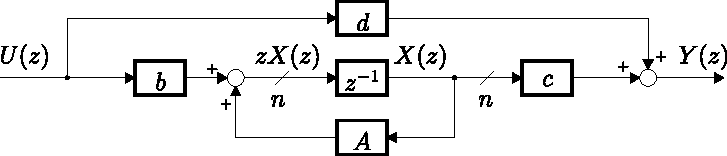
\includegraphics[width=\columnwidth, align=t]{images/diskrete_ZRD.pdf}
\end{minipage}
\hfill
\begin{minipage}[c]{0.35\columnwidth}
        \fbox{\parbox{0.9\columnwidth}{
            \vspace{-0.3cm}
            \begin{align*}
                x(k+1)  &= \bm{A} \cdot x(k) + b \cdot u(k) \\
                y(k)    &= b \cdot x(k) + d \cdot u(k)
            \end{align*}
            \vspace{-0.5cm}
    }}
\end{minipage}


\subsubsection{UTF aus diskreter ZRD}

\begin{minipage}[c]{0.44\columnwidth}
    Die diskrete UTF $G(z)$ kann jedoch eindeutig aus der ZRD bestimmt werden
\end{minipage}
\hfill
\begin{minipage}[c]{0.52\columnwidth}
    $$ G(z) = c \cdot (z \bm{I} - \bm{A})^{-1} \cdot b + d $$
\end{minipage}


\subsection{Stabilität}{245}

Das zeitdiskrete System ist \textbf{asymptotisch stabil}, wenn \textbf{alle Pole innerhalb des Einheitskreises liegen} (bzw. $\abs{z} < 1$ ist). \\
Unter Betrachtung der ZRD wird diese Bedingung interpretiert als:
Wenn alle \textbf{Eigenwerte} der \textbf{Systemmatrix} $\bm{A}$ (welche den Eigenwerten von $\bm{\Lambda} = \bm{A_{\rm Diag}}$ entsprechen)
einen \textbf{Betrag $< 1$} besitzen, ist das System \textbf{asymptotisch stabil}.

\vspace{-0.2cm}

$$ \boxed{ \det(\lambda \cdot \bm{I} - \bm{A}) \overset{!}{=} 0 \qquad \rightarrow \forall \lambda \quad  \abs{\lambda} < 1 \qquad \text{ \textrightarrow\ System asymptotisch stabil}}  $$

\textbf{Achtung: Umgekehrt gilt diese Aussage nicht!} Ein asymptotisch stabiles System bedeutet \textbf{nicht}, 
dass alle Eigenwerte der Systemmatrix $\bm{A}$ des Systems einen Betrag $< 1$ haben \textrightarrow\ Pol-/Nullstellenkürzungen


\subsection{Steuerbarkeit}{245}

\begin{outline}
    \1 Es gelten die (fast) äquivalenten Definitionen wie in zeitkontinuierlichen Systemen
    \1 Die Steuerbarkeit des Systems wird mit der Steuerbarkeitsmatrix bestimmt
\end{outline}


\subsubsection{Steuerbarkeitsmatrix $\bm{Q_S}$}

Ein System ist \textbf{vollständig steuerbar}, wenn
\begin{outline}
    \1 Der \textbf{Rang} der Steuerbarkeitsmatrix $\bm{Q_S}$ der Ordnung $n$ des Systems entspricht
        \2 Die Matrix $\bm{Q_S}$ hat somit vollen Rang
    \1 Bei Single-Input-System: ($m = 1$): Die \textbf{Determinante} von $\bm{Q_S}$ \textbf{ungleich Null ist}
\end{outline}

\vspace{-0.1cm}

$$
\boxed{ 
\bm{Q_S} = 
\begin{bmatrix}
    \bm{B} & \bm{A B} & \bm{A^2 B} & \cdots & \bm{A^{n-1} B} 
\end{bmatrix}
\qquad \qquad \text{ Dimension: } n \times (n \cdot m)
}
$$

\begin{minipage}[c]{0.48\columnwidth}
    \begin{tabular}{ll}
        $\bm{A}$    & Systemmatrix ($n \times n$)   \\
        $\bm{B}$    & Eingangsmatrix ($n \times m$) \\
    \end{tabular}
\end{minipage}
\hfill
\begin{minipage}[c]{0.48\columnwidth}
    \begin{tabular}{ll}
        $n$         & Zustände \\
        $m$         & Eingänge \\
    \end{tabular}
\end{minipage}


\subsection{Beobachtbarkeit}{245}

\begin{outline}
    \1 Es gelten die (fast) äquivalenten Definitionen wie in zeitkontinuierlichen Systemen
    \1 Die Beobachtbarkeit des Systems wird mit der Beobachtbarkeitsmatrix bestimmt
\end{outline}


\subsubsection{Beobachtbarkeitsmatrix $\bm{Q_B}$}

Ein System ist \textbf{vollständig beobachtbar}, wenn

\begin{outline}
    \1 Der \textbf{Rang} der Beobachtbarkeitsmatrix $\bm{Q_B}$ der Ordnung $n$ des Systems entspricht
        \2 Die Matrix $\bm{Q_B}$ hat somit vollen Rang
    \1 Bei Single-Output-System:  Die \textbf{Determinante} von $\bm{Q_B}$ \textbf{ungleich Null ist}
\end{outline}

\smallskip

\begin{minipage}[c]{0.4\columnwidth}
    $$
    \bm{Q}_B = 
    \begin{bmatrix}
        \bm{C} \\ \bm{C A} \\ \bm{C A^2} \\ \vdots \\ \bm{C A^{n-1}} 
    \end{bmatrix}
    $$
\end{minipage}
\hfill
\begin{minipage}[c]{0.58\columnwidth}
    \begin{tabular}{ll}
        Dimension:  & $(k \cdot n) \times n$ \\
        $\bm{A}$    & Systemmatrix ($n \times n$) \\
        $\bm{C}$    & Beobachtungsmatrix ($k \times m$) \\
        $n$         & Zustände \\
        $m$         & Eingänge \\
        $k$         & Ausgänge 
    \end{tabular}
\end{minipage}


\columnbreak


        \section{Direkter digitaler Reglerentwurf}

Beim direkten Reglerentwurf wird die Strecke $G_S(s)$ in zeitdiskrete Form $\overline{G}_S(z)$ gebracht.
Anschliessend wird für $\overline{G}_S(z)$ ein (zeitdiskreter) Regler $G_{\rm R, D}(z)$ entworfen.


\subsection{Direkter digitaler Reglerentwurf -- Vorgehen}

Das Vorgehen und die Berechnungen sind grundsätzlich gleich wie im zeitkontinuierlichen Bereich, weshalb in folgender Abbildung der Platzhalter $\cdot$ für $s$ oder $z$ verwendet ist.
Es müssen jedoch einige Voraussetzungen erfüllt sein.

\vspace{-0.2cm}

\begin{center}
    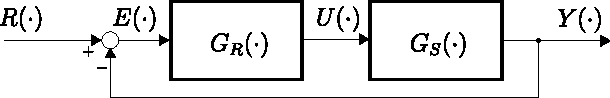
\includegraphics[width=0.75\columnwidth, align=t]{images/direkt_dig_reg_regelkreis.pdf}
\end{center}

$$ \text{Geschlossener Regelkreis} \quad  G_f(\cdot) = \frac{Y(\cdot)}{R(\cdot)} = \frac{G_S(\cdot) G_R(\cdot)}{1 + G_S(\cdot)G_R(\cdot)} $$


\subsubsection{Voraussetzungen}

\begin{outline}
    \1 Alle involvierten Teilsysteme müssen \textbf{'kompatibel'} sein
        \2 Entweder alles in $z$ formuliert oder alles in $s$ formuliert
    \1 Zeitdiskrete Systeme müssen \textbf{dieselbe Abtastzeit} haben
\end{outline}



\subsection{ZOH-Diskretisierung -- Überblick}
\label{ZOH-Diskretisierung -- Überblick}

Eine ZOH-Diskretisierung kann an einer UTF oder im Zustandsraum durchgeführt werden:

\vspace{-0.2cm}

\begin{center}
    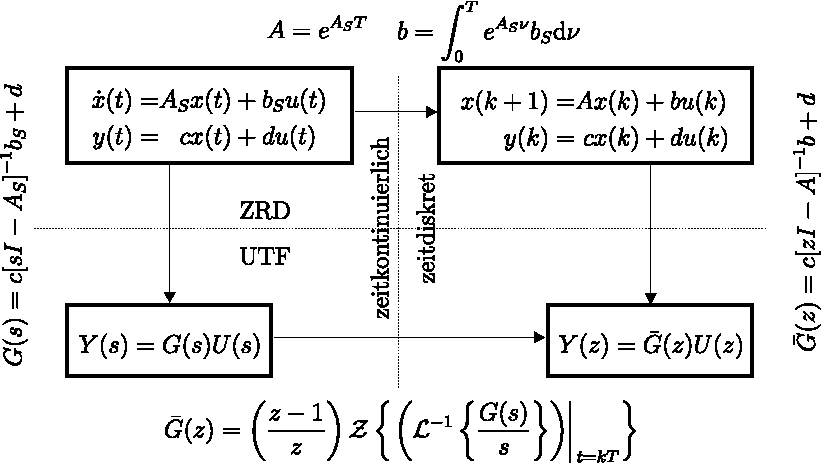
\includegraphics[width=0.9\columnwidth, align=t]{images/direkt_dig_reg_ZOH_konversion.pdf}
\end{center}

Beide Diskretisierungs-Arten werden in den Abschnitten \ref{ZOH-Diskretisierung mit UTF} und \ref{ZOH-Diskretisierung im Zustandsraum} genauer beschrieben.


\subsubsection{Steuerbarkeit / Beobachtbarkeit}{251-253}

Für Steuerbarkeit und Beobachtbarkeit bei der ZOH-Diskretisierung gilt:

\smallskip

\begin{outline}
    \1 Solange die Abtatzeit $T$ \textbf{sinnvoll gewählt} wird, bleiben diese Eigenschaften \textbf{erhalten}
    \1 Ein System kann durch Diskretisierung \textbf{nicht} steuerbar / beobachtbar \textbf{gemacht werden}
\end{outline}


\subsubsection{Stabilität}

Für die Stabilität gilt bei der ZOH-Diskretisierung:

\smallskip

\begin{outline}
    \1 Stabilität \textbf{bleibt} bei ZOH-Diskretisierung \textbf{erhalten}
        \2 Pole bzw. Eigenwerte gehorchen bei ZOH-Diskretisierung der Abbildung $z = e^{sT}$
\end{outline}

\smallskip


\paragraph{Abbildung $\bm{z = e^{sT}$}}

\begin{center}
    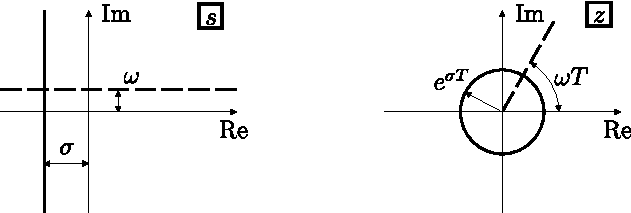
\includegraphics[width=0.8\columnwidth, align=t]{images/direkt_dig_reg_abbildung_geraden.pdf}
\end{center}


\begin{ctabular}{ccc}
    \toprule
    $\bm{s}$\textbf{-Ebene}             & \textlrarrow  & $\bm{z}$\textbf{-Ebene}       \\
    \midrule
    Gerade mit konstantem Imaginärteil  & \textlrarrow  & Halbgerade durch Nullpunkt    \\
    \midrule
    Geraden mit konstantem Realteil     & \textlrarrow  & Kreise um den Nullpunkt       \\
    \midrule
    Imaginärachse                       & \textlrarrow  & Einheitskreis                 \\
    \midrule
    Linke Halbebene                     & \textlrarrow  & Innerhalb des Einheitskreises \\
    \midrule
    Nullpunkt (Ursprung)                & \textlrarrow  & Punkt $(1 \, | \, 0)$         \\
    \bottomrule
\end{ctabular}


\example{Abblidung eines Streifens}

\begin{center}
    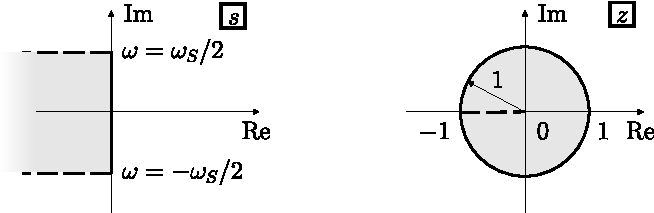
\includegraphics[width=0.8\columnwidth, align=t]{images/direkt_dig_reg_abbildung_beispiel.pdf}
\end{center}

\vspace{-0.2cm}


\subsection{ZOH-Diskretisierung mit UTF}{248-249}
\label{ZOH-Diskretisierung mit UTF}

Eine zeitkontinuierliche Strecke $G_S(s) = G(s)$ wird mit einem ZOH-Glied (zero-order-hold) \textbf{exakt} diskretisiert, weil der Eingang  zur zeitdiskreten Strecke als stückweise konstant angenommen werden kann.

\begin{minipage}[c]{0.78\columnwidth}
    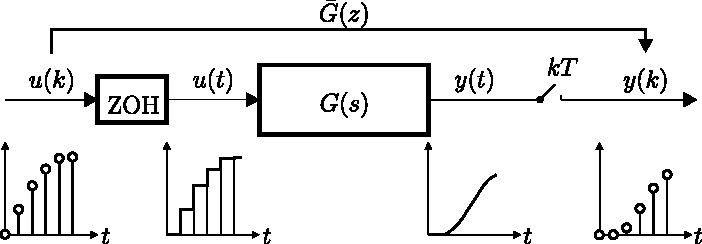
\includegraphics[width=\columnwidth, align=t]{images/direkt_dig_reg_ZOH_diskretisierung.pdf}
\end{minipage}
\hfill
\begin{minipage}[c]{0.2\columnwidth}
    $$ \overline{G}(z) = \frac{Y(z)}{U(z)} $$
\end{minipage}

\smallskip

Im Gegenzug zur ZOH-Diskretisierung ist die Approximation der Strecke mittels z.B. Tustin beim indirekten Reglerentwurf nicht exakt!


\subsubsection{Bestimmung der diskreten Stecke $\bm{\overline{G}_S(z)}$}

Die Bestimmung von $\overline{G}_S(z)$ wird vereinfacht durch Betrachtung der \textbf{Impulsantwort}. \\
Mit $u(k) = \{ 1, \, 0, \, 0, \, 0, \, \ldots \}$ ergibt sich am Ausgang die Impulsantwort $y(k) = g(k)$, deren \\
z-Transformierte $ G(z) \, (= \overline{G}_S(z))$ ist.

\smallskip

Als Formel kann die diskrete UTF $\overline{G}_S(z)$ ermittelt werden als:
\vspace{-0.2cm}
$$ \boxed{ \overline{G}_S(z)    = \left(\frac{z-1}{z} \right) \, \mathcal{Z} \left\{ \left( \mathcal{L}^{-1} \left\{ \frac{G_S(s)}{s} \right\} \right) \Bigg|_{t = kT} \right\}
                                = (1 - z^{-1}) \, \mathcal{Z} \left\{ \left( \mathcal{L}^{-1} \left\{ \frac{G_S(s)}{s} \right\} \right) \Bigg|_{t = kT} \right\} } $$
                       

\example{ZOH-Diskretisierung mit UTF}

Eine gegebene Strecke $G_S(s) = \frac{1}{s^2}$ soll mittels ZOH diskretisiert werden. 
Es soll also $\overline{G}_S(z)$ bestimmt werden, indem obige Formel Schritt für Schritt angewendet wird.
\vspace{-0.2cm}
\[
    \underbrace{ \frac{1}{s^2} }_{G_S(s)} \
    \underrightarrow{\div s} \quad 
    \frac{1}{s^3} \quad 
    \underrightarrow{\mathcal{L}^{-1}} \quad 
    \frac{t^2}{2} \quad
    \underrightarrow{t = kT} \quad 
    \frac{k^2 T^2}{2} \quad
    \underrightarrow{\mathcal{Z}} \quad 
    \frac{T^2}{2} \frac{z (z+1)}{(z-1)^3} \quad
    \underrightarrow{\cdot \left( \frac{z-1}{z} \right)} \quad 
    \underbrace{ \frac{T^2}{2} \frac{(z+1)}{(z-1)^2}}_{\overline{G}_S(z)}
\]

\vspace{-0.4cm}

\subsection{ZOH-Diskretisierung im Zustandsraum}{250-251}
\label{ZOH-Diskretisierung im Zustandsraum}

Eine zeitkontinuierliche ZRD kann in eine zeitdiskrete ZRD umgewandelt werden (entspricht dem Weg 'rechts herum' in Abschnitt \ref{ZOH-Diskretisierung -- Überblick}).
Die Variablen des Zustandsvektors bleiben bei der Diskretisierung erhalten, werden jedoch nur noch zum Abtastzeitpunkt evaluiert.

\smallskip

Die diskrete ZRD kann dargestellt werden als:

\vspace{-0.2cm}

\begin{minipage}[c]{0.4\columnwidth}
    \begin{align*}
        x(k+1)  &= \bm{A} \cdot x(k) + b \cdot u(k) \\
        y(k)    &= c \cdot x(k) + d \cdot u(k)
    \end{align*}
\end{minipage}
\hfill
\begin{minipage}[c]{0.58\columnwidth}
    \[
        \bm{A}  = e^{\bm{A_S} T} \qquad
        b       = \int\limits_0^T e^{\bm{A_S} \nu} \, \diff \nu \cdot b_S
    \]
\end{minipage}

\smallskip

\textbf{Hinweis:} $\bm{A_S}$ und $b_S$ entsprechen den zeit\myul{kontinuierlichen} ZRD-Werten 


\subsubsection{Bestimmung der diskreten Stecke $\bm{\overline{G}_S(z)}$}

Die diskrete UTF der Strecke $\bm{\overline{G}_S(z)}$ kann aus der diskreten ZRD ähnlich wie im zeitkontinuierlichen Bereich bestimmt werden:
\vspace{-0.2cm}
$$ \overline{G}_S(z) = c \cdot (z \bm{I} - \bm{A})^{-1} \cdot b + d $$


\subsection{Reglerentwurf -- WOK}{254}

Basierend auf den Pole / Nullstellen des offeren Regelkreises werden die Pole / Nullstellen des geschlossenen Regelkreises (bzw. die Pole des Reglers) platziert.
Da das Zeichnen der WOK (des \textbf{geschlossenen} Regelkreises) analog zum zeitkontinuierlichen Bereich erfolgt, wird dies hier nicht weiter erläutert (\textrightarrow\ siehe Anhang Abschnitt \ref{Wurzelortskurven (WOK)}).

\smallskip

Die (zeitdiskrete) UTF des geschlossenen Regelkreises mit einem P-Regler mit Verstärkung $K$ ergibt sich als
\vspace{-0.2cm}
$$ G_f(z) = \frac{K \cdot G_S(z)}{1 + K \cdot G_S(z)} = \frac{ K \cdot \frac{Z_S(z)}{N_S(z)} }{1 + K \cdot \frac{Z_S(z)}{N_S(z)}}
    = \frac{K \cdot Z_S(z) }{ \underbrace{N_S(z) + K \cdot Z_S(z) }_{\text{char. Polynom } N_f(s)} } = \frac{Z_f(z)}{N_f(z)} $$


Wird ein dynamischer Regler verwendet, so wird $G_0(z)$ in die \textbf{mathematisch verlangte Form} von aufgeteilt.
\vspace{-0.2cm}
$$ G_f(z) = \frac{G_R(z) \cdot G_S(z)}{1 + G_R(z) \cdot G_S(z)} = \frac{ \frac{Z_R(z)}{N_R(z)} \cdot \frac{Z_S(z)}{N_S(z)} }{1 + \frac{Z_R(z)}{N_R(z)} \cdot \frac{Z_S(z)}{N_S(z)}}
    = \frac{Z_R(z) \cdot Z_S(z) }{ \underbrace{N_R(z) \cdot N_S(z) + Z_R(z) \cdot Z_S(z) }_{\text{char. Polynom } N_f(s)} } = \frac{Z_f(z)}{N_f(z)} $$


\begingroup
\fbox{\parbox{0.97\columnwidth}{
    \raggedright
    \textbf{Hinweis:} Die Methode zur \textbf{Wurzel-Bestimmung} funktioniert für \textbf{jedes Polynom} $\bm{N_f(s)}$ (oder auch $N_f(z)$), wenn dieses in 
    die verlangte Form gebracht werden kann (und auch nur dann)!

    \vspace{-0.2cm}

    $$ N_f(s) = P_N(s) + \text{Faktor} \cdot P_Z(s) = N(s) + K \cdot Z(s) $$
}}
\endgroup

\smallskip

\textbf{Hinweis:} Wie eine WOK (in $s$) gezeichnet wird kann dem Anhang (Abschnitt \ref{Zeichnen von Wurzelortskurven}) entnommen werden.


\subsubsection{Platzierung der Pole}

\begin{outline}
    \1 Pole \textbf{innerhalb des Einheitskreises} platzieren ($\abs{z} < 1$)
    \1 Gebiet, welches Spezifikation erfüllt in z-Ebene transformieren und Pole innerhalb des transformierten Gebiets platzieren
    \1 Es können Interatoren (mit Polen bei $z = 1$) in den Regelkreis eingebaut werden
        \2 Somit wird der stationäre Fehler unterdrückt
\end{outline}


\subsection{Reglerentwurf -- Vorgabe des geschl. Regelkreises}{256-257}

Bei bekannter \textbf{diskreten} Regelstrecke $G_S(z)$ kann die benötigte UTF des Reglers $G_R(z)$ ermittelt werden, wenn die UTF des geschlossenen Regelkreises $G_f(z)$ vorgegeben ist.

\vspace{-0.2cm}

$$ G_f(z) = \frac{G_0(z)}{1 + G_0(z)} \quad \text{ \textlrarrow\ } \quad  G_0(z) = \frac{G_f(z)}{1 - G_f(z)}  \quad \text{und  } G_R(z) = \frac{G_0(z)}{G_S(z)}  $$


Daraus folgt für die UTF $G_R(z)$ des diskreten Reglers: 

\vspace{-0.1cm}

$$ \boxed{ G_R(z) = \frac{Z_f(z)}{N_f(z) - Z_f(z)} \cdot \frac{N_S(z)}{Z_S(z)} } \qquad \text{mit } G_S(z) = \frac{Z_S(z)}{N_S(z)} \text{ und  } G_f(z) = \frac{Z_f(z)}{N_f(z)} $$


\para{Bemerkungen}

\begin{outline}
    \1 Die Strecke $G_S(z)$ darf \textbf{keine} Pole ausserhalb des Einheitskreises haben
    \1 Die Strecke darf keine NS ausserhalb des Einheitskreises haben, ausser wenn dise in $G_f(z)$ übernommen werden
    \1 Die Strecke darf \textbf{Totzeiten} (ganzzahlige Vielfache der Abtastzeit) haben: $T_t = N \cdot T$
        \2 Stecke erhält dadurch $N$ zusätzliche Pole im Ursprung: $G_S(z) = \ldots \cdot z^{-N}$
    \1 Der relative Grad (\textbf{Polüberschuss}) der vorgegebenen UTF $G_f(z)$ muss mindestens so gross sein wie derjenige der Strecke $G_S(z)$
        \2 Regler ist sonst nicht realisierbar
\end{outline}
$$ \underbrace{ \mathrm{Ord}\{ N_S(z) \} - \mathrm{Ord}\{ Z_S(z) \} }_{\text{Polüberschuss Strecke}} \leq \underbrace{ \mathrm{Ord} \{N_f(z) \} - \mathrm{Ord} \{ Z_f(z) \} }_{\text{Polüberschuss geschl. System}} $$



\subsection{Reglerentwurf -- Deadbeat-Regler}{256-257}

Ein Deadbeat-Regler wird bei einem Führungsschritt der \textbf{Fehler in endlich vielen Abtastschritten Exakt zu Null}.
Der geschlossene Regelkreis $G_f(z)$ besetzt somit folgende Eigenschaften:

\begin{ctabular}{ll}
    \tabitem Alle Pole bei $z = 0$  & \tabitem Statische Verstärkung $G_f(1) = 1$
\end{ctabular}


\subsubsection{Einfachster Deadbeat-Regler}

Damit der Fehler zu Null, wird ist integrierendes Verhalten nötig. 
Der eifachste mögliche Regler $G_R(z)$ und der geschlossene Regelkreis $G_f(z)$ besitzen also die folgenden UTFs:

$$ G_R(z) = \frac{1}{z-1} \cdot \frac{1}{G_S(z)} \qquad \qquad \Rightarrow\ G_f(z) = \frac{1}{z} $$

Natürlich muss der Regler realisierbar sein (stabil, relativer Grad von $G_S$)


\subsection{Reglerentwurf -- Zustandsraum}{257-258}

Beim Reglerentwurf im Zustandsraum sind bei zeitdiskreten Systemen dieselben drei Komponenten von Interesse wie in zeitkontinuierlichen Systemen:

\smallskip

\begin{outline}
    \1 \textbf{Beobachter}, der den Zustandsvektor schätzt
    \1 \textbf{Zustandsrückführung}, die z.B. die Strecke stabilisiert
    \1 \textbf{Vorverstärkung}, für die statische Verstärkung \textrightarrow\ $G_f(1) = 1$
\end{outline}

\smallskip

Da die Konzepte weitgehend vom zeitkontinuierlichen Bereich übernommen werden können, werden nur ausgewählte Aspekte erwähnt.


\subsubsection{Polplatzierung}

\begin{outline}
    \1 Die Eigenwerte von $\bm{A} - \bm{BK}$ (und somit die Pole des Systems) ( \textrightarrow\ Zustandsrückführung) bzw. $\bm{A} - \bm{HC}$ ( \textrightarrow\ Beobachter) müssen nun innerhalb des Einheitskreises platziert werden
    \1 Es können dieselben Matlab-Funktionen verwendet werden wie bei einem zeitkontinuierlichen System
    \1 Separationsprinzip bleibt erhalten
\end{outline}


\subsubsection{LQR / LQG}

\begin{outline}
    \1 Es wird eine andere Zielfunktion $J$ optimiert, was zu einer anderen Ricatti-Gleichung führt
        \2 Mathematischer Lösungsweg ist anders
    \1 Matlab benötigt einen anderen Befehl: $\mylstbox{dlqr(...)}$ statt $\mylstbox{lqr(...)}$
\end{outline}



        
        %\pagebreak
        \part{Anhang}
        \section{Mathemathik-Hilfen}

\subsection{Trigonometrie}

% Copy-Paste from KomFour

\begingroup
\renewcommand{\arraystretch}{2}
\setlength{\tabcolsep}{0mm}
\scalebox{0.33}{
\Huge
\begin{tabularx}{3\columnwidth}{rp{1mm}V{3}*{17}{C}}
    \rowcolor{subsectioncolor!30}$\bm{\alpha}$\phantom{${}^{\circ}$} && $0$ & $\dfrac{\pi}{6\mathstrut}$ & $\dfrac{\pi}{4}$ & $\dfrac{\pi}{3}$ & $\dfrac{\pi}{2}$ & $\dfrac{2\pi}{3}$ & $\dfrac{3\pi}{4}$ & $\dfrac{5\pi}{6}$ & $\pi$ & $\dfrac{7\pi}{6}$ & $\dfrac{5\pi}{4}$ & $\dfrac{4\pi}{3}$ & $\dfrac{3\pi}{2}$ & $\dfrac{5\pi}{3}$ & $\dfrac{7\pi}{4}$ & $\dfrac{11\pi}{6}$ & $2\pi$ \\\hline
    \rowcolor{subsectioncolor!30}$\bm{\alpha^\circ}$ && \phantom{${}^\circ$}$0^\circ$ & $30^\circ$ & $45^\circ$ & $60^\circ$ & $90^\circ$ & $120^\circ$ & $135^\circ$ & $150^\circ$ & $180^\circ$ & $210^\circ$ & $225^\circ$ & $240^\circ$ & $270^\circ$ & $300^\circ$ & $315^\circ$ & $330^\circ$ & $360^\circ$ \\\hline
    $\bm{\sin(\alpha)}$ && $0$ & $\dfrac{1}{2\mathstrut}$ & $\dfrac{\sqrt{2}}{2}$ & $\dfrac{\sqrt{3}}{2}$ & $1$ & $\dfrac{\sqrt{3}}{2}$ & $\dfrac{\sqrt{2}}{2}$ & $\dfrac{1}{2}$ & $0$ & $-\dfrac{1}{2}$ & $-\dfrac{\sqrt{2}}{2}$ & $-\dfrac{\sqrt{3}}{2}$ & $-1$ & $-\dfrac{\sqrt{3}}{2}$ & $-\dfrac{\sqrt{2}}{2}$ & $-\dfrac{1}{2}$ & $0$ \\\hline
    $\bm{\cos(\alpha)}$ && $1$ & $\dfrac{\sqrt{3}}{2\mathstrut}$ & $\dfrac{\sqrt{2}}{2}$ & $\dfrac{1}{2}$ & $0$ & $-\dfrac{1}{2}$ & $-\dfrac{\sqrt{2}}{2}$ & $-\dfrac{\sqrt{3}}{2}$ & $-1$ & $-\dfrac{\sqrt{3}}{2}$ & $-\dfrac{\sqrt{2}}{2}$ & $-\dfrac{1}{2}$ & $0$ & $\dfrac{1}{2}$ & $\dfrac{\sqrt{2}}{2}$ & $\dfrac{\sqrt{3}}{2}$ & $1$ \\\hline
    $\bm{\tan(\alpha)}$ && $0$ & $\dfrac{\sqrt{3}}{3\mathstrut}$ & $1$ & $\sqrt{3}$ & $\pm\infty$ & $-\sqrt{3}$ & $-1$ & $-\dfrac{\sqrt{3}}{3}$ & $0$ & $\dfrac{\sqrt{3}}{3}$ & $1$ & $\sqrt{3}$ & $\pm\infty$ & $-\sqrt{3}$ & $-1$ & $-\dfrac{\sqrt{3}}{3}$ & $0$ \\\hline
    $\bm{\cot(\alpha)}$ && $\pm\infty$ & $\sqrt{3}$ & $1$ & $\dfrac{\sqrt{3}}{3\mathstrut}$ & $0$ & $-\dfrac{\sqrt{3}}{3}$ & $-1$ & $-\sqrt{3}$ & $\pm\infty$ & $\sqrt{3}$ & $1$ & $\dfrac{\sqrt{3}}{3}$ & $0$ & $-\dfrac{\sqrt{3}}{3}$ & $-1$ & $-\sqrt{3}$ & $\pm\infty$ \\
\end{tabularx}}
\endgroup


\subsection{Lineare Algebra -- Repetition}

Der Anhang B des Skripts (S. 279 ff.) beschreibt die Matrizenrechnung. Hier werden nur einige Ausschnitte erwähnt.


\subsubsection{Matrixmultiplikation}

Die Spaltenzahl von $\bm{A}$ muss mit der Zeilenzahl von $\bm{B}$ übereinstimmen! \\
Dimensionen: $\bm{A} \in \mathbb{C}^{m \times n}, \, \bm{B} \in \mathbb{C}^{n \times p} \quad \Rightarrow\ \bm{C} \in \mathbb{C}^{m \times p}$


\example{Matrixmultiplikation}
% Beispiel von LinAlg
$A =
	\begin{pmatrix}
		\crd{1} & \crd{2}   & \crd{4}   \\
		0       & 4         & -1
	\end{pmatrix}$, \qquad 
$B =
	\begin{pmatrix}
		\cbl{-2}    & 4     \\
		\cbl{-4}    & -5    \\
		\cbl{2}     & 4
	\end{pmatrix}$
	
\smallskip

$C = A \cdot B =
	\begin{pmatrix}
		\crd{1} \cdot ({\cbl{-2}}) + {\crd{2}} \cdot ({\cbl{-4}}) + \crd{4} \cdot \cbl{2}   &
		\crd{1} \cdot 4 + \crd{2} \cdot (-5) + \crd{4} \cdot 4                              \\
		0 \cdot ({\cbl{-2}}) + 4 \cdot (\cbl{-4}) + (-1) \cdot \cbl{2}                      &
		0 \cdot 4 + 4 \cdot (-5) + (-1) \cdot 4
	\end{pmatrix}
    = 
    \begin{pmatrix}
		-2  & 10    \\
        -18 & -24
	\end{pmatrix}$


\subsubsection{Übersicht zu (quadratischen) Matritzen}

Die Aussagen innerhalb einer Spalte sind jeweils äquivalent.

\begin{ctabular}{l c l}
    \toprule
    $A \in \mathbb{C}^{n \times n}$ ist regulär         & & $A \in \mathbb{C}^{n \times n}$ ist singulär            \\
    \midrule
    $\det(A) \neq 0$                                    & & $\det(A) = 0$                                           \\
    \midrule
    Die Inverse $A^{-1}$ existiert                      & & Die Inverse $A^{-1}$ existiert \textbf{nicht}           \\
    \midrule
    $n$ Spaltenvektoren von $A$                         & & $n$ Spaltenvektoren von $A$ sind                        \\
    sind linear unabhängig                              & & \textbf{nicht} linear unabhängig                        \\
    \midrule
    $n$ Zeilenvektoren von $A$                          & & $n$ Zeilenvektoren von $A$                              \\
    sind linear unabhängig                              & & sind \textbf{nicht} linear unabhängig                   \\
    \midrule
    $A$ hat vollen Rang:                                & & $A$ hat \textbf{nicht} vollen Rang:                     \\
    $\mathrm{rang}(A) = n$                              & & $\mathrm{rang}(A) < n$                                  \\
    \bottomrule
\end{ctabular}

\textrightarrow\ Die oberen drei Zeilen gelten \textbf{nur für quadratische Matritzen}


\subsubsection{Determinante}

Die Determinante ist nur für \textbf{quadratische} Matritzden definiert

\smallskip

\begin{minipage}[c]{0.38\columnwidth}
    \begin{itemize}
        \item $A = \begin{bmatrix} 
                        a_{11} 
                    \end{bmatrix} 
                    \quad \Rightarrow \det(A) = a_{11}$
    \end{itemize}
\end{minipage}
\hfill
\begin{minipage}[c]{0.6\columnwidth}
    \begin{itemize}
        \item $A = \begin{bmatrix}
                        a_{11}  & a_{12}    \\
                        a_{21}  & a_{22}
                    \end{bmatrix}
                    \quad \Rightarrow \det(A) = a_{11} a_{22} - a_{12} a_{21}$ 
    \end{itemize}
\end{minipage}


\begin{minipage}[c]{0.38\columnwidth}
    \begin{itemize}
        \item $A = \begin{bmatrix}
                        a_{11}  & a_{12}    & a_{13}    \\
                        a_{21}  & a_{22}    & a_{23}    \\
                        a_{31}  & a_{32}    & a_{33}    
                    \end{bmatrix}$
    \end{itemize}
\end{minipage}
\hfill
\begin{minipage}[c]{0.6\columnwidth}
    \begin{align*}
        \Rightarrow \det(A) &= a_{11} a_{22} a_{33} + a_{12} a_{23} a_{31} + a_{13} a_{21} a_{32}\\
                            &- a_{11} a_{23} a_{32} - a_{12} a_{21} a_{33} - a_{13} a_{22} a_{31}
    \end{align*}
\end{minipage}

\smallskip

\begin{itemize}
    \item Bei einer Diagonalmatrix oder einer Dreieicksmatrix entspricht die Determinante dem Produkt der Diagonalelemente
\end{itemize}


\subsubsection{Singuläre / Reguläre Matritzen}

\begin{itemize}
    \item Eine Matrix $A \in \mathbb{C}^{n \times n}$ ist singulär, falls $\det(A) = 0$
    \item Eine Matrix $A \in \mathbb{C}^{n \times n}$ ist regulär, falls $\det(A) \neq 0$
\end{itemize}


\subsubsection{Rang einer Matrix}

\begin{itemize}
    \item Der Rang einer Matrix $A \in \mathbb{C}^{m \times n}$ bestimmt sich als Anzahl linear unabhängiger Spaltenvektoren
        (was zugleich der Anzahl linear unabhängiger Zeilenvektoren ist)
    \item Der Maximal mögliche Rang ist $\min(m, \,n)$
\end{itemize}



\subsubsection{Inverse Matritzen}

Eine Matrix ist invertierbar, wenn sie regulär ist.

\smallskip

\begin{minipage}[c]{0.38\columnwidth}
    $A = \begin{bmatrix} 
            a_{11} 
        \end{bmatrix} 
        \quad \Rightarrow A^{-1} = \frac{1}{a_{11}}$
\end{minipage}
\hfill
\begin{minipage}[c]{0.6\columnwidth}
    $A = \begin{bmatrix}
            a_{11}  & a_{12}    \\
            a_{21}  & a_{22}
        \end{bmatrix}
        \quad \Rightarrow A^{-1} = \frac{1}{\det(A)} \begin{bmatrix}
                                        a_{22}      & - a_{12}    \\
                                        - a_{21}    & a_{11}
                                        \end{bmatrix}$
\end{minipage}

\smallskip

\begin{itemize}
    \item Für $n \geq 3$ empfiehlt sich der Gauss-Jordan Algorithmus
    \item Die Inverse von Diagonalmatritzen kann durch Inversion der Diagonalelemente berechnet werden
\end{itemize}
%------------------ neu ------------------
\subsubsection{Permutationsmatrix}

Eine Permutationsmatrix $P \in \mathbb{R}^{n \times n}$ entsteht durch Vertauschen von
Zeilen der Einheitsmatrix. Es gilt:
\[
P^{-1} = P^T, \qquad P^T P = I
\]

Eine Rotation um den Winkel $\alpha$ wird beschrieben durch:
\[
R(\alpha) =
\begin{pmatrix}
\cos\alpha & -\sin\alpha \\
\sin\alpha & \cos\alpha
\end{pmatrix}
\]
Eigenwerte:
\[
\lambda_{1,2} = e^{\pm j\alpha}
\]
Reell nur für $\alpha = k\pi$.
%-----------------------------------------------

\subsubsection{Lineare Gleichungssysteme lösen}

\vspace{-0.2cm}

$$ \bm{A} \cdot \vec{x} = \vec{b} \quad \Leftrightarrow \quad \vec{x} = \bm{A^{-1}} \cdot \vec{b} $$
%----------------------- neu ------------------
Ein lineares Gleichungssystem $A x = b$ besitzt genau dann eine eindeutige Lösung, wenn
\[
\det(A) \neq 0 \quad \Leftrightarrow \quad \mathrm{rang}(A) = n
\]
In diesem Fall gilt:
\[
x = A^{-1} b
\]
%-----------------------------------------------
\subsubsection{Transformationen}

\begin{minipage}[c]{0.7\columnwidth}
    \raggedright
    Die Transformationsmatrix $\bm{T}$ kann eine Drehung, Rotation, Projektion oder Permutation von $\vec{p}$ verursachen. \\
    Permutation: Reihenfolge ändern (\textrightarrow\ Permutationsmatritzen haben nur eine 1 pro Zeile und Spalte und sind orthagonal)
\end{minipage}
\hfill
\begin{minipage}[c]{0.25\columnwidth}
    $$ \vec{q} = \bm{T} \cdot \vec{p} $$
\end{minipage}



\subsubsection{Eigenwerte / Eigenvektoren}

Um die Eigenwerte $\lambda_i$ einer (quadratischen) Matrix $\bm{A}$ zu berechnen, muss die folgende Gleichung erfüllt sein:
$$ \det(\lambda \cdot \bm{I} - \bm{A}) \overset{!}{=} 0 $$
Die Lösungen dieser charakteristischen Gleichung entsprechen den Eigenwerten $\lambda_i$.

\smallskip

Die Eigenvektoren berechnen sich durch Einsetzen von $\lambda_i$ in die Gleichung(en)
$$ (\lambda_i \bm{I} - \bm{A}) \cdot \vec{v}_i = \vec{0} $$
\textrightarrow\ Eine Koordinate muss gewählt werden, die andere Koordinate ist linear abhängig!

\medskip


\para{Eigenschaften von Eigenwerten und Eigenvektoren}

\begin{outline}
    \1 Bei einer Diagonalmatrix / Dreiecksmatrix entsprechen die Diagonalelemente $a_{ii}$ den Eigenwerten
    \1 Eine singuläre Matrix hat mindestens einen Eigenwert bei Null
    \1 Zwei Eigenwerte $\lambda_i \neq \lambda_j$ haben unabhängig Eigenvektoren $\vec{v}_i$ und $\vec{v}_j$
    \1 Die Eigenwerte von $\bm{A}$ und $\bm{A^{\tps}}$ sind identisch
    \1 Reelle Eigenwerte haben reelle Eigenvektoren
\end{outline}
%----------------------- neu ------------------
\para{Geometrische Interpretation von Eigenvektoren}
Für $A v = \lambda v$ gilt:
\begin{itemize}
\item $|\lambda| > 1$: Streckung
\item $|\lambda| < 1$: Stauchung
\item $\lambda < 0$: Spiegelung
\end{itemize}

\para{Typische Zustandswahl}

Translation:

\[
    x=
    \begin{bmatrix}
        s\\
        \dot s
    \end{bmatrix}
\]

Rotation:

\[
    x=
    \begin{bmatrix}
        \varphi\\
        \dot\varphi
    \end{bmatrix}
\]
%-----------------------------------------------

\subsubsection{Positive Definitheit von Matritzen}

Die Definitheit einer Matrix kann auf mehrere Arten überprüft werden.
Eine Matrix $\bm{Q}$ ist positiv definit ($\bm{Q} > 0$), wenn

\smallskip

\begin{minipage}[t]{0.48\columnwidth}
    \begin{outline}
        \1 \textbf{Alle} Eigenwerte der Matrix grösser Null sind \textrightarrow\ $\lambda_i > 0$
        \1 \textbf{Alle} führenden Hauptminoren positiv sind
            \2 Alle Determinanten der gezeigten 'Untermatritzen' müssen $> 0$ sein
    \end{outline}
\end{minipage}
\hfill
\begin{minipage}[t]{0.48\columnwidth}
    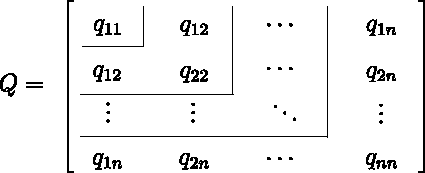
\includegraphics[width=\columnwidth, align=t]{images/hauptminoren.pdf}
\end{minipage}
%==========================================================================================================
\subsubsection{Lagrange-Verfahren}

\[
L=T-V
\]

\[
\frac{d}{dt}
\left(
\frac{\partial L}{\partial \dot q_i}
\right)
-
\frac{\partial L}{\partial q_i}
=
Q_i
\]

Ohne äussere Kräfte gilt:

\[
Q_i=0
\]

\vspace{0.1cm}

\textbf{Vorgehen:}

\begin{enumerate}
    \item $T$ bestimmen
    \item $V$ bestimmen
    \item $L=T-V$
    \item Lagrange-Gleichung anwenden
    \item DGL $\rightarrow$ ZRD $\rightarrow$ Linearisierung
\end{enumerate}
%===============================================================================

\subsubsection{Exponentialfunktion von Matritzen}
\label{Exponentialfunktion von Matritzen}

Die Exponentialfunktion von Matritzen berechnet sich aus der Definition der Taylor-Reihe.

$$ e^{\bm{A} t} = \bm{I} + \bm{A} t + \frac{\bm{A}^2}{2!} t^2 + \cdots + \frac{\bm{A}^k}{k!} t^k + \cdots 
    = \sum\limits_{k=0}^{\infty} \frac{\bm{A}^k t^k}{k!} $$


\paragraph{Spezialfall: Diagonalmatrix}

\vspace{-0.2cm}

$$
\bm{A} = 
\begin{bmatrix}
    a_{11}  & 0         & \cdots    & 0         \\
    0       & \ddots    & \ddots    & \vdots    \\
    \vdots  & \ddots    & \ddots    & 0         \\
    0       & \cdots    & 0         & a_{nn}
\end{bmatrix}
\quad \Rightarrow \quad
e^{\bm{A} t} =
\begin{bmatrix}
    e^{a_{11} \cdot t}  & 0         & \cdots    & 0                 \\
    0                   & \ddots    & \ddots    & \vdots            \\
    \vdots              & \ddots    & \ddots    & 0                 \\
    0                   & \cdots    & 0         & e^{a_{nn} \cdot t}
\end{bmatrix}
$$
%----------------------- neu ------------------
\subsubsection{MATLAB-Hinweis}
\[
A * B \text{ (Matrixmultiplikation)}, \qquad
A .* B \text{ (elementweise Multiplikation)}
\]
%-----------------------------------------------

\subsection[Dezibel \deci \bel]{Dezibel $\boldsymbol{\deci \bel$}}

\vspace{-0.2cm}

$$ \boxed{ |K|_{\deci \bel} = 20 \, \deci \bel \cdot \log_{10} |K| \quad \Leftrightarrow \quad 
            |K| = 10 ^{\big( \frac{|K|_{\deci \bel}}{20 \, \deci \bel}\big)}  } $$

\textbf{Hinweis:} Die Betragsstrichte nur Notation! $|K|$ kann sehr wohl negativ sein!


\subsubsection{Rechenregeln}

\begin{itemize}
    \item Multiplikation \textrightarrow\ Addition 
        \vspace{-0.2cm}
        $$ | K_1 \cdot K_2 |_{\deci \bel} = | K_1 |_{\deci \bel} + | K_2 |_{\deci \bel} $$
    \item Division \textrightarrow\ Subtraktion 
        $$ \Big| \frac{K_1}{K_2} \Big|_{\deci \bel} = | K_1 |_{\deci \bel} - | K_2 |_{\deci \bel} $$
    \item Kehrwert \textrightarrow\ Negatives Vorzeichen 
        $$ \Big| \frac{1}{K_1} \Big|_{\deci \bel} = | 1 |_{\deci \bel} - | K_1 |_{\deci \bel} = - | K_1 |_{\deci \bel} $$
\end{itemize}


\subsubsection[\deci \bel--Umrechnungstabelle]{$\boldsymbol{\deci \bel}$--Umrechnungstabelle}{133}

\begin{minipage}[c]{0.48\columnwidth}
    \begin{ctabular}{c c}
        \toprule
        \textbf{Faktor $\boldsymbol{[1]}$}  & \textbf{Dezibel $\boldsymbol{\deci \bel}$} \\
        \midrule
        $100$                   & $40$  \\ 
        $10$                    & $20$  \\
        $1$                     & $0$   \\
        $0.1$                   & $-20$ \\
        $0.01$                  & $-40$ \\
        \bottomrule
    \end{ctabular}
\end{minipage}
\hfill
\begin{minipage}[c]{0.48\columnwidth}
    \begin{ctabular}{c c}
        \toprule
        \textbf{Faktor $\boldsymbol{[1]}$}  & \textbf{Dezibel $\boldsymbol{\deci \bel}$} \\
        \midrule
        $2$                     & $6$   \\
        $\sqrt{2}$              & $3$   \\
        $\frac{1}{\sqrt{2}}$    & $-3$  \\
        $\frac{1}{2}$           & $-6$  \\
        \bottomrule
    \end{ctabular}
\end{minipage}


\subsection{Spezielle Ansätze PBZ}

\vspace{-0.2cm}

\renewcommand{\arraystretch}{2}
\begin{tabular}{ll}
    $f(x)$  & $ = \frac{5x^2-37x+54}{x^3-6x^2+9x} = \frac{A}{x}+\frac{B}{x-3}+\frac{C}{(x-3)^2} = \frac{A(x-3)^2+Bx(x-3)+Cx}{x(x-3)^2}$ \\ 
    $f(x)$  & $ = \frac{1.5x}{x^3-6x^2+12x-8} = \frac{A}{x-2}+\frac{B}{(x-2)^2}+\frac{C}{(x-2)^3 } =\frac{A(x-2)^2+B(x-2)+C}{(x-2)^3}$  \\
    $f(x)$  & $ = \frac{x^2-1}{x^3+2x^2-2x-12} = \frac{A}{x-2}+\frac{Bx+C}{x^2+4x+6} = \frac{A(x^2+4x+6)+(Bx+C)(x-2)}{(x-2)(x^2+4x+6)}$ \\
\end{tabular}
\renewcommand{\arraystretch}{1}


%\columnbreak

\subsection{Laplace-Transformation}
\label{Laplace-Transformation}


\subsubsection{Laplace-Transformierte einiger Funktionen}{21}
\label{Laplace-Transformierte einger Funktionen}

Alle Funktionen $f(t)$ sind implizit mit dem Einheitssprung $\varepsilon(t)$ multipliziert, sodass die Funktionen nur
für $t \geq 0$ definiert sind.

\vspace{0.2cm}

\begin{minipage}[t]{0.48\columnwidth}
    \begin{center}
        \renewcommand{\arraystretch}{1.4}
        \begin{tabular}{c c c}
            \toprule
            $\bm{f(t)}$                             & $\laplace$    & $\bm{F(s)}$                   \\
            \midrule
            $\delta(t)$                             & $\laplace$    & $1$                           \\
            \midrule
            $\delta(t - T_t)$                       & $\laplace$    & $e^{-T_t s}$                  \\
            \midrule
            $\varepsilon(t)$                        & $\laplace$    & $\frac{1}{s}$                 \\
            \midrule
            $t$                                     & $\laplace$    & $\frac{1}{s^2}$               \\
            \midrule            
            $t^2$                                   & $\laplace$    & $\frac{2}{s^3}$               \\
            \midrule
            $t^n$                                   & $\laplace$    & $\frac{n!}{s^{n+1}}$          \\
            \midrule   
            $e^{at}$                                & $\laplace$    & $\frac{1}{s-a}$               \\  
            \midrule
            $t \cdot e^{at}$                        & $\laplace$    & $\frac{1}{(s-a)^2}$           \\
            \bottomrule
        \end{tabular}
        \renewcommand{\arraystretch}{1}
    \end{center}
\end{minipage}
\hfill
\begin{minipage}[t]{0.48\columnwidth}
    \begin{center}
        \renewcommand{\arraystretch}{1.4}
        \begin{tabular}{c c c}
            \toprule
            $\bm{f(t)}$                             & $\laplace$    & $\bm{F(s)}$                   \\
            \midrule
            $t^n \cdot e^{at}$                      & $\laplace$    & $\frac{n!}{(s-a)^{n+1}}$      \\
            \midrule
            $\sin(bt)$                              & $\laplace$    & $\frac{b}{s^2 + b^2}$         \\
            \midrule
            $\cos(bt)$                              & $\laplace$    & $\frac{s}{s^2 + b^2}$         \\          
            \midrule
            $1 - e^{at}$                            & $\laplace$    & $\frac{-a}{s (s-a)}$          \\
            \midrule
            $e^{at} \cdot \cos(bt)$                 & $\laplace$    & $\frac{s-a}{(s-a)^2 + b^2}$   \\
            \midrule
            $e^{at} \cdot \sin(bt)$                 & $\laplace$    & $\frac{b}{(s-a)^2 + b^2}$     \\
            \midrule
            $\frac{e^{at} - e^{bt}}{a-b}$           & $\laplace$    & $\frac{1}{(s-a)(s-b)}$        \\
            \midrule
            $\frac{a \, e^{at} - b \, e^{bt}}{a-b}$ & $\laplace$    & $\frac{s}{(s-a)(s-b)}$        \\
            \bottomrule
        \end{tabular}
        \renewcommand{\arraystretch}{1}
    \end{center}
\end{minipage}

\vspace{0.2cm}

\textbf{Hinweis:} Der Einheitssprung $\varepsilon(t)$ äussert sich als eine $1$ in der Gleichung im Zeitbereich \\
\textbf{Hinweis:} Teilweise braucht es Umformungen, damit die Tabelle angewendet werden kann


\subsubsection{Eigenschaften der Laplace-Transformation}{22}

\resizebox{\columnwidth}{!}{
    \begin{tabular}{ccc}
        \toprule
        \textbf{Zeitbereich}                                                        & \textbf{Bildbereich}                          & \textbf{Operation im Zeitbereich}     \\
        \midrule
        $a_1 f_1(t) + a_2 f_2(t)$                                                   & $a_1 F_1(s) + a_2 F_2(s)$                     & Superposition                         \\
        \midrule
        $\dot{f}(t)$                                                                & $s F(s) - f(0)$                               & Differentiation ...                   \\
        \midrule
        $\ddot{f}(t)$                                                               & $s^2 F(s) - s f(0) - \dot{f}(0)$              & ...mehrfach angewendet                \\
        \midrule
        $\int_{0}^{t} f(\tau) \, \diff \tau$                                        & $\frac{1}{s} F(s)$                            & Integration                           \\
        \midrule
        $f(t - T_t) \quad [T_t \text{ reell, } \geq 0]$                             & $F(s) \cdot e^{- T_t \, s}$                   & Rechtsverschiebung                    \\
        \midrule
        $f_1(t) * f_2(t) = \int_{0}^{t} f_1(\tau) \cdot f_2(t - \tau) \, \diff t$   & $F_1(s) \cdot F_2(s)$                         & Faltung                               \\
        \midrule
        $f(a \cdot t) \quad [a \text{ reell, } > 0]$                                & $\frac{1}{a} \cdot F \Big( \frac{s}{a} \Big)$ & Skalierung                            \\
        \midrule
        $e^{\mp at} \cdot f(t)$                                                     & $F(s \pm a)$                                  & Dämpfung                              \\
        \bottomrule
    \end{tabular}
}

\subsubsection{Grenzwertsätze der Laplace-Transformation}{22}

\textbf{Achtung:} Grenzwertsätze dürfen nur angewendet werden, wenn Grenzwerte existieren!

\smallskip

\begin{itemize}
    \item Das Anfangswerttheorem gilt für Regelungstechniker immer
    \item Das Endwerttheorem gilt \textbf{nur}, wenn \textbf{System stabil} ist \\
        (Polstellen in linker Halbebene bzw. $\sigma < 0$)
\end{itemize}

\begin{center}
    \begin{tabular}{l c ll}
        \toprule
        \textbf{Zeitbereich}                &       & \textbf{Bildbereich}                          & \textbf{Bezeichnung}      \\
        \midrule
        $\lim\limits_{t \to 0} f(t)$        & $=$   & $\lim\limits_{s \to \infty} s \cdot F(s)$     & Anfangswerttheorem        \\
        \midrule
        $\lim\limits_{t \to \infty} f(t)$   & $=$   & $\lim\limits_{s \to 0} s \cdot F(s)$          & Endwerttheorem            \\
        \bottomrule
    \end{tabular}
\end{center}



\section{Wurzelortskurven (WOK)}
\label{Wurzelortskurven (WOK)}

% WOK aus RegT3
\subsection{Grundsätzliches Aussehen der WOK}

\begin{outline}
    \1 Char. Polynom $N_f(s) = N(s) + K \cdot Z(s)$ hat für jeden $K$-Wert $n$ Wurzeln (Nullstellen)
        \2 Visualisiert: $n$ kontinuierliche Linien (Äste)
    \1 WOK ist immer \textbf{symmetrisch} bezüglich der \textbf{reellen Achse}
    \1 Für $K = 0$ sind die $n$ Wurzeln von $N_f(s)$ und $N(s)$ identisch und entsprechen den $n$ Polen von $G(s)$
    \1 Anfangspunkte der Äste: $n$ Wurzeln von $N(s)$ \textrightarrow\ Kreuze
    \1 Endpunkte der Äste: $m$ Wurzeln von $Z(s)$ \textrightarrow\ Kreise \\
        $n-m$ Äste laufen ins Unendliche
\end{outline}


\subsection{Zeichnen von Wurzelortskurven}{96-98}
\label{Zeichnen von Wurzelortskurven}

\para{1. Pol- / Nullstellenplan}

Pole / Nullstellen von $G(s)$ werden in komplexer Zahlenebene eingetragen:

\vspace{0.1cm}

\begin{outline}
    \1 Pole $p_k$ ($k=1 \ldots n$) werden als $\times$ dargestellt \textrightarrow\ Startpunkte der $n$ Äste
    \1 Nullstellen $z_k$ ($k=1 \ldots m$) werden als $\circ$ dargestellt \textrightarrow\ Endpunkte von $m$ Ästen
\end{outline}

\medskip


\para{2. Reelle Achse}

\begin{enumerate}
    \item Start 'ganz rechts' (weiter rechts als alle Einträge $\times$ bzw. $\circ$) auf reeller Achse starten; Stift 'nicht schreibend' bzw 'oben'
    \item Nach links wandern und bei \textbf{jedem} $\times$ bzw. $\circ$ Stift toggeln \\
        ('nicht schreibend' \textlrarrow\ 'schreibend') \\
        \textrightarrow\ Doppel-Pole bzw. Doppel-Nullstellen entsprechend einem Punkt ('Doppel-Toggel')
\end{enumerate}

\begin{center}
    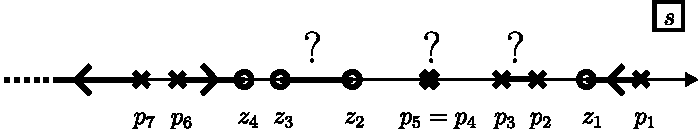
\includegraphics[width=0.78\columnwidth]{images/WOK_zeichnen_reelle_achse.pdf}
\end{center}

\textbf{ \textrightarrow\ Gültige WOK-Äste verbinden einen Pol mit einer Nullstelle.} \\
An den Stellen mit ? (Verbindung von Pol zu Pol bzw. NS zu NS) ist die Situation noch unbefriedigend, da $n > m$. \textrightarrow\ siehe 3. und 4. 

\medskip


\para{3. Asymptoten: Schnittpunkte und Richtungen}

Wenn $n > m$ gilt, dann streben $n-m$ Äste (\textbf{Geraden}) der WOK asymptotisch gegen Unendlich. Zu berechnen ist der \textbf{Schnittpunkt} und 
die \textbf{Richtung der ersten der Asymptoten}. Die weiteren Asymptoten sind dann \textbf{gleichmässig} versetzt.

\smallskip

\begin{minipage}{0.7\columnwidth}
    $$ \text{Schnittpunkt:} \quad \sigma_A = \frac{\sum_{k=1}^{n} \Re{p_k} - \sum_{k=1}^{m} \Re{z_k}}{n-m} $$
\end{minipage}
\hfill
\begin{minipage}{0.28\columnwidth}
    \begin{tabular}{@{}ll@{}}
        $n$ & \# Pole   \\
        $m$ & \# NS 
    \end{tabular}
\end{minipage}

\vspace{0.1cm}

$$ \text{Richtung 1. Asymptote} \quad \phi = \frac{\pi}{n-m} \qquad 
    \text{gleichmässig versetzt um} \quad \frac{2 \pi}{n-m} $$

\begin{center}
    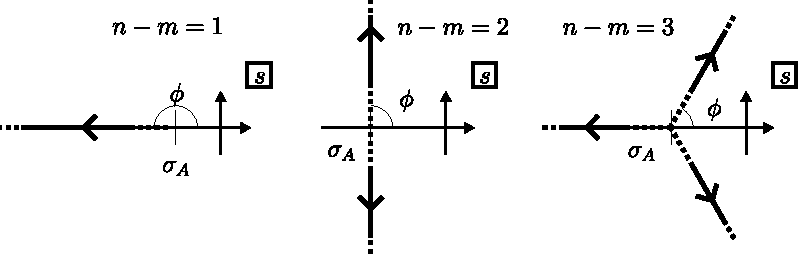
\includegraphics[width=0.8\columnwidth]{images/WOK_asymptoten.pdf}
\end{center}

\vspace{-0.2cm}

\textrightarrow\ Wenn $n-m$ ungerade, dann geht immer eine Asymptote auf reeller Achse nach links

\medskip


\para{4. Verzweigungspunkte / Vereinigungspunkte}

Bei Verbindung von Pol zu Pol bzw. NS zu NS treten Verzweigungen / Vereinigungen auf. In diesen Punkten gilt Folgendes:

\vspace{0.1cm}

\begin{outline}
    \1 Äste treten (meist) \textbf{rechtwinklig aus der reellen Achse} aus.
    \1 Verzweigungspunkt bzw. Vereinigungspunkt befindet sich \textbf{in der Mitte} des Pol- bzw. NS-Paares
    \1 Die \textbf{Form} der betreffenden Äste kann auf zwei Arten verlaufen:
        \2 Kreisförmig in Richtung \textbf{Asymptoten}, welche in der Nähe sind
        \2 Kreisförmig zum nächsten Verzweigungspunkt bzw. Vereinigungspunkt
\end{outline}

\begin{center}
    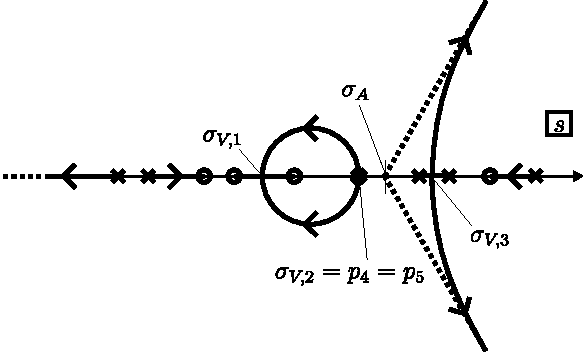
\includegraphics[width=0.7\columnwidth]{images/WOK_komplett.pdf}
\end{center}

\vspace{-0.2cm}

\begin{minipage}[c]{0.58\columnwidth}
    Die genauen Verzweigungspunkte / Vereinigungspunkte können auch mittels folgender impliziter Formel berechnet werden:
\end{minipage}
\hfill
\begin{minipage}[c]{0.4\columnwidth}
    $$ \underbrace{ \sum\limits_{k=1}^{n} \frac{1}{\sigma_V - p_k} }_{\text{Pole}} =
        \underbrace{ \sum\limits_{k=1}^{m} \frac{1}{\sigma_V - z_k} }_{\text{Nullstellen}} $$
\end{minipage}

\vspace{0.1cm}

\textbf{Achtung:} Die Formel kann unbrauchbare Lösungen (z.B. mit $\Im{\sigma_{V,i}} \neq 0$) liefern, welche 'aussortiert' werden müssen.


\subsection{WOK zu einigen geläufigen Pol- / NS-Verteilungen}{99}

\begin{center}
    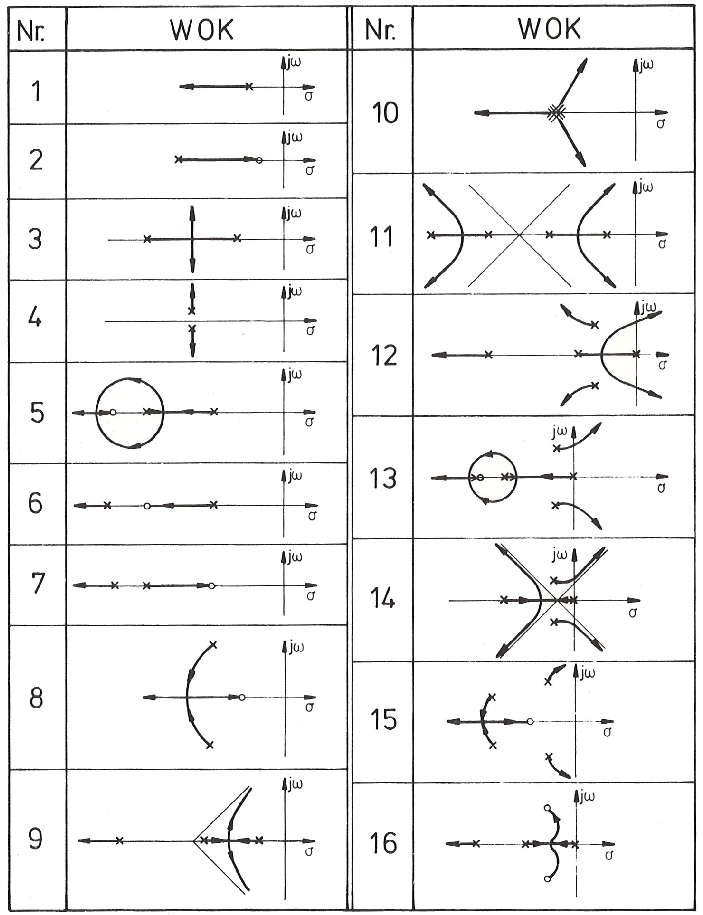
\includegraphics[width=0.9\columnwidth]{images/WOK_pol_NS_tabelle.pdf}
\end{center}



\subsection{Auslegen eines staischen P-Reglers mittels WOK}{{101-102}}

\subsubsection{Vorgehen -- P-Regler mit WOK auslegen}
\label{Vorgehen -- P-Regler mit WOK auslegen}

\begin{enumerate}
    \item WOK skizzieren (inkl. Dämpfung) gemäss Abschnitt \ref{Zeichnen von Wurzelortskurven}
    \item Pole, welche bei variablem $K$ auf Asymptoten wandern so platzieren, dass gewünschte \textbf{Dämpfung} erreicht ist
    \item \textbf{Bandbreite} $\bm{\omega_n}$ und \textbf{Verstärkung} $\bm{K}$ bestimmen, indem einer der in 2. platzierten Pole betrachtet wird \\
        Dabei werden von einem solchen Pol aus \textbf{Verbindungslinien} zu allen weiteren Polen ($\theta_i$) und allen Nullstellen ($\lambda_i$) gezeichnet.
        Die Verstäkung $K$ berechnet sich dann aus den entsprechenden \textbf{Abständen} $\theta_i$ und $\lambda_i$ gemäss
        $$ \boxed{ K = \frac{\prod_{i=1}^{n} \theta_i}{\prod_{i=1}^{m} \lambda_i} = \frac{\theta_1 \cdot \theta_2 \cdot \ldots \cdot \theta_n}{\lambda_1 \cdot \lambda_2 \cdot \ldots \cdot \lambda_m} } $$
        \textrightarrow\ Falls keine Nullstellen vorhanden sind, ist das entsprechende Produkt $=1$
    \item Weitere Verstärkungen (z.B. $K_R$) aus $K$ bestimmen
\end{enumerate}


\example{Auslegung eines P-Regler mittels WOK}

Eine (stabile) Strecke $G_S(s)$ soll mit einem P-Regler mit $G_R(s) = K_R$ mit \textbf{möglichst grosser 
Verstärkung} $\bm{K_R}$ geregelt werden, wobei alle Pole eine \textbf{minimale Dämpfung} $\bm{\zeta = 0.7}$ haben sollen.

\vspace{0.1cm}

Der offene Regelkreis $G_0(s)$ wird betrachtet als

\vspace{-0.1cm}

$$ G_0(s) = K_R \cdot \underbrace{ \frac{5}{s^2 + 6s + 8} }_{G_S(s)} 
    = \underbrace{K_R \cdot 5}_{K} \cdot \underbrace{ \frac{1}{s^2 + 6s + 8}}_{G_S(s)}  $$

Gemäss Abschnitt \ref{Vorgehen -- P-Regler mit WOK auslegen} kann nun der Regler ausgelegt werden und somit $K_R$ aus $K$ bestimmt werden.

\vspace{0.1cm}

\begin{minipage}[t]{0.3\columnwidth}
    \begin{center}
        \myul{\textbf{1. WOK skizzieren}}
    \end{center}

    \vspace{-0.2cm}

    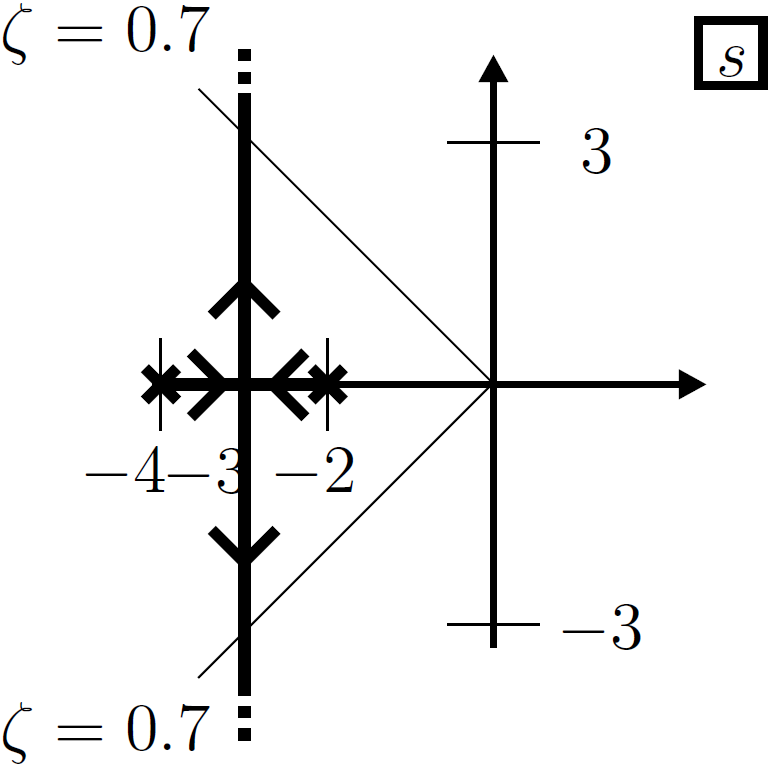
\includegraphics[width=\columnwidth, align=t]{images/WOK_P-Regler_WOK_zeichnen.png}
\end{minipage}
\hfill
\begin{minipage}[t]{0.3\columnwidth}
    \begin{center}
        \myul{\textbf{2. Pole platzieren}}
    \end{center}

    \vspace{-0.2cm}

    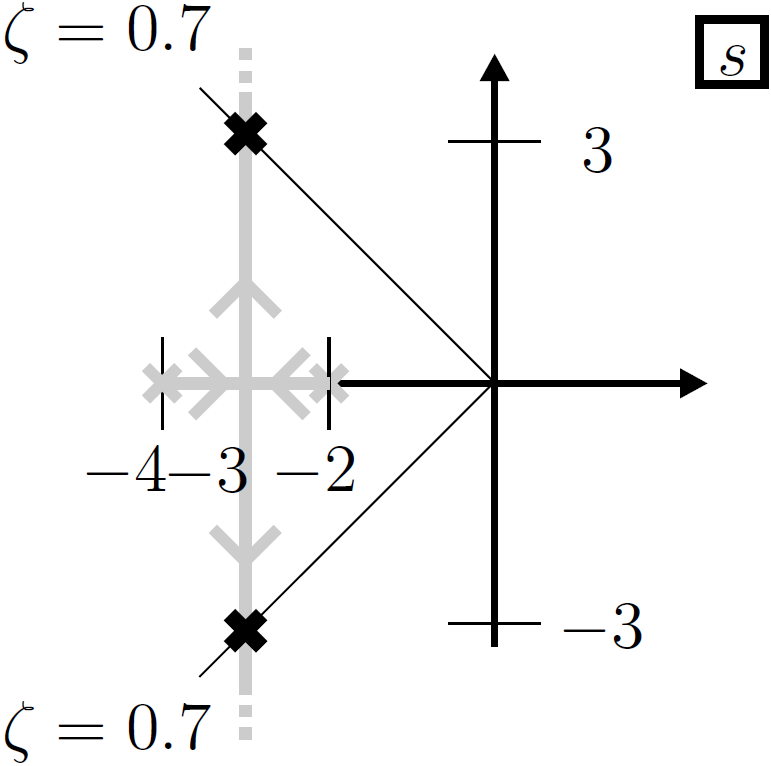
\includegraphics[width=\columnwidth, align=t]{images/WOK_P-Regler_daempfung.png}
\end{minipage}
\hfill
\begin{minipage}[t]{0.3\columnwidth}
    \begin{center}
        \myul{\textbf{3. $\bm{K}$ und $\bm{\omega_n}$ bestimmen}}
    \end{center}
    
    \vspace{-0.2cm}

    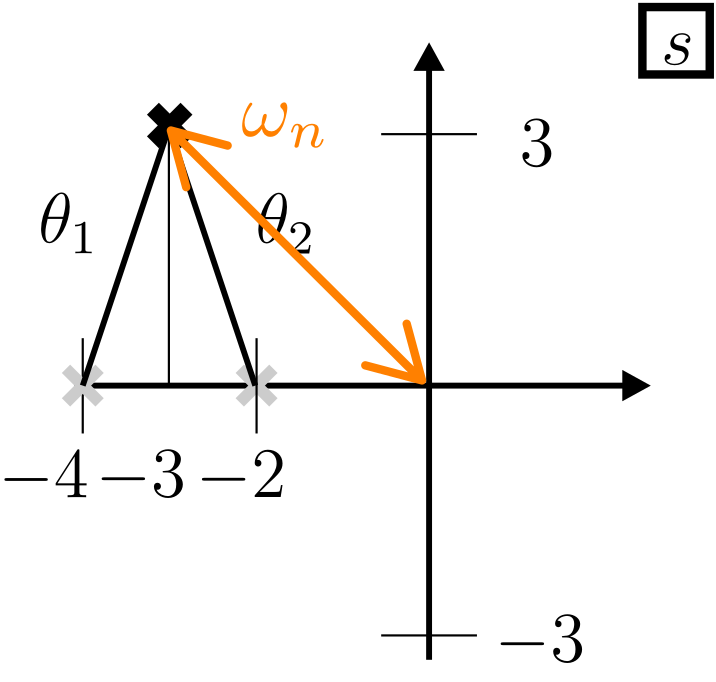
\includegraphics[width=\columnwidth, align=t]{images/WOK_P-Regler_verstaerkung.png}
\end{minipage}

\vspace{0.1cm}

\myul{\textbf{4. $\bm{K_R}$ bestimmen}}

Aus $K = \theta_1 \cdot \theta_2 = \sqrt{1^2 + 3^2} \cdot \sqrt{1^2 + 3^2} = 10$ und $K = 5 \cdot K_R$ ergibt sich $K_R = 5$


\subsubsection{Beantwortung der 'Grundfragen' für P-Regler}

\begin{itemize}
    \item Regelkreis ist stabil, wenn $K$ gross genug gewählt wird, dass alle Pole in RHE sind
    \item Bandbreite: $\omega_n$ aus WOK abgelesen: $\omega_n = \sqrt{3^2 + 3^2} = \sqrt{2 \cdot + 3^2} = \sqrt{2} \cdot 3 \, \frac{\radian}{\second}$
    \item Gewünschte Dämpfung $\zeta = 0.7$ ist einstellbar (Pole konnten so platziert werden)
    \item Stationärer Fehler: $e_{\infty} = \frac{E(s)}{R(s)} = \frac{1}{1 + G_0} \Big|_{s = 0} =\frac{4}{9}$
\end{itemize}


%\columnbreak

\section{Matlab}

\subsection{Zustandsraumdarstellung (ZRD)}

\subsubsection{Zustandsraum-Objekte (LTI-Objekte)}

\lstinputlisting[aboveskip=1mm, belowskip=0mm]{snippets/LTI-Objekte.m}


\subsubsection{Spezielle Matritzen im Zustandsraum}

\lstinputlisting[aboveskip=1mm, belowskip=0mm]{snippets/spezielle_matritzen_zustandsraum.m}


\subsection{Bode- und Nyquist}

\lstinputlisting[aboveskip=1mm, belowskip=0mm]{snippets/bode_nyquist.m}


\subsection{z-Transformation}

\lstinputlisting[aboveskip=1mm, belowskip=0mm]{snippets/z_transformation.m}


\subsection{Implementation eines diskreten Reglers}

\lstinputlisting[aboveskip=1mm, belowskip=0mm]{snippets/digitale_regler.m}


\subsection{Wurzelortskurven}

\lstinputlisting[aboveskip=1mm, belowskip=0mm]{snippets/wurzelortskurven.m}


\subsection{Zustandsrückführungen / Beobachter}

\lstinputlisting[aboveskip=1mm, belowskip=0mm]{snippets/zustandsrueckfuehrung.m}




\section{Statische Grundglieder (ohne Gedächtnis)}

Der Ausgang des Systems ist \textbf{nur} vom aktuellen Eingang abhängig 
$$ y(t) = f( u(t) ) $$
\textbf{Hinweis:} $u(t)$ entspricht meist $A \cdot \varepsilon(t)$ (skalierter Einheitssprung)


\subsection{P-Glied (Proportional)}

\vspace{-0.2cm}

$$ \boxed{ y(t) = K \cdot u(t) } $$

\begin{minipage}{0.23\columnwidth}
    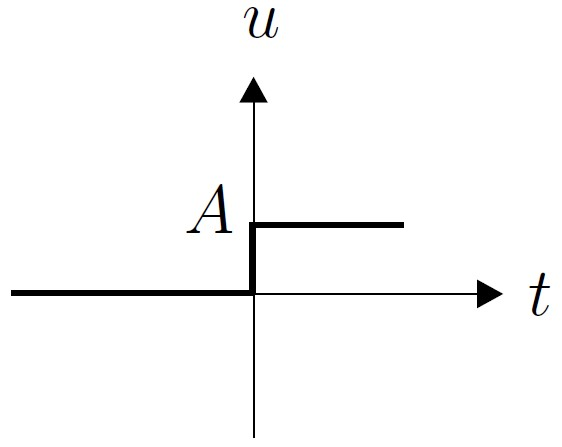
\includegraphics[width=0.8\columnwidth]{images/RegT1_grundglieder/eingangssignal_schrittantwort} 
\end{minipage}
\hfill
\begin{minipage}{0.23\columnwidth}
    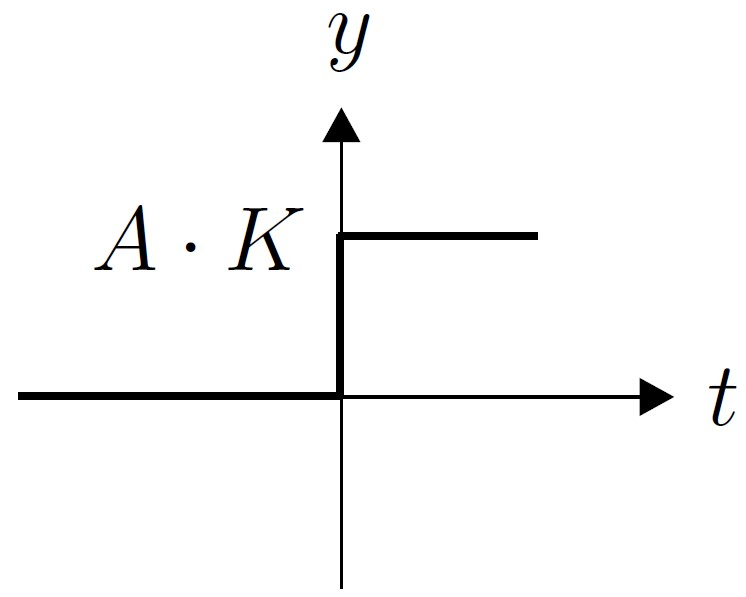
\includegraphics[width=0.8\columnwidth]{images/RegT1_grundglieder/schrittantwort_p-glied} 
\end{minipage}
\hfill
\begin{minipage}{0.23\columnwidth}
    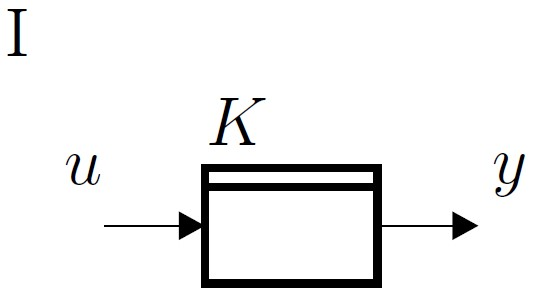
\includegraphics[width=0.8\columnwidth]{images/RegT1_grundglieder/symbol_p-glied_1}
\end{minipage}
\hfill
\begin{minipage}{0.23\columnwidth}
    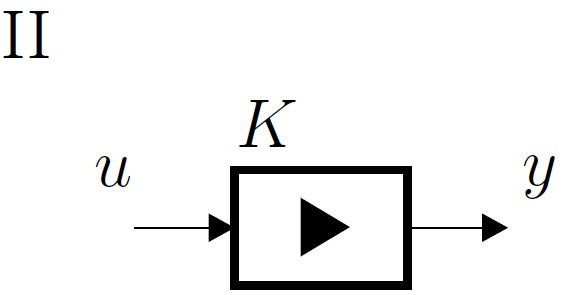
\includegraphics[width=0.8\columnwidth]{images/RegT1_grundglieder/symbol_p-glied_2}
\end{minipage}


\section{Dynamische Grundglieder (mit Gedächtnis)}

Der Ausgang des Systems ist vom aktuellen \textbf{und} von vergangenen Eingängen abhängig.
Vergangene Eingänge werden im System in einem Speicher, einem Zustand $x(t)$ abgelegt. 
$$ y(t) = f( u(t), \, x(t) ) $$


\subsubsection{Prozesse mit / ohne Ausgleich}

\begin{tabular}{ll}
ohne Ausgleich:     & Sprungantwort wächst grenzenlos an \\
mit Ausgleich:      & Sprungantwort strebt gegen endlichen Wert \\
				    & \textrightarrow\ \textbf{Gegenkopplung} am Ausgang
\end{tabular}


\subsection{Totzeit-Glied}

\vspace{-0.2cm}

$$ \boxed{ y(t) =  u(t - T_t) }  $$

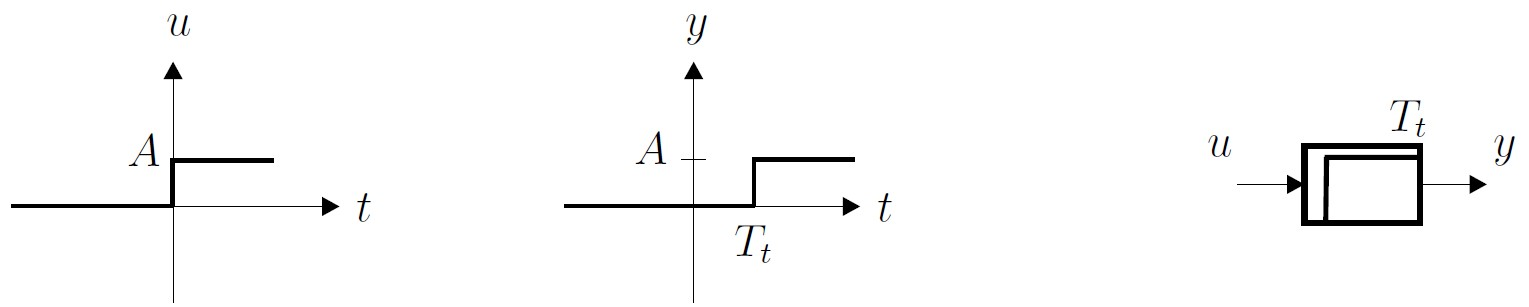
\includegraphics[width=0.9\columnwidth]{images/RegT1_grundglieder/totzeit-glied}


\subsection{I-Glied (Integrierer)}

\begin{minipage}{0.48\columnwidth}
    $$ \boxed{ \text{DGL: } \dot{y}(t) = K \cdot u(t) }  $$
\end{minipage}
\hfill
\begin{minipage}{0.48\columnwidth}
    $$ \boxed{ \scriptstyle{ y = \int\limits_{- \infty}^t u(\tau) \, \diff \tau = K \int\limits_{- \infty}^t u(\tau) \, \diff \tau + y(0) } }$$
\end{minipage}

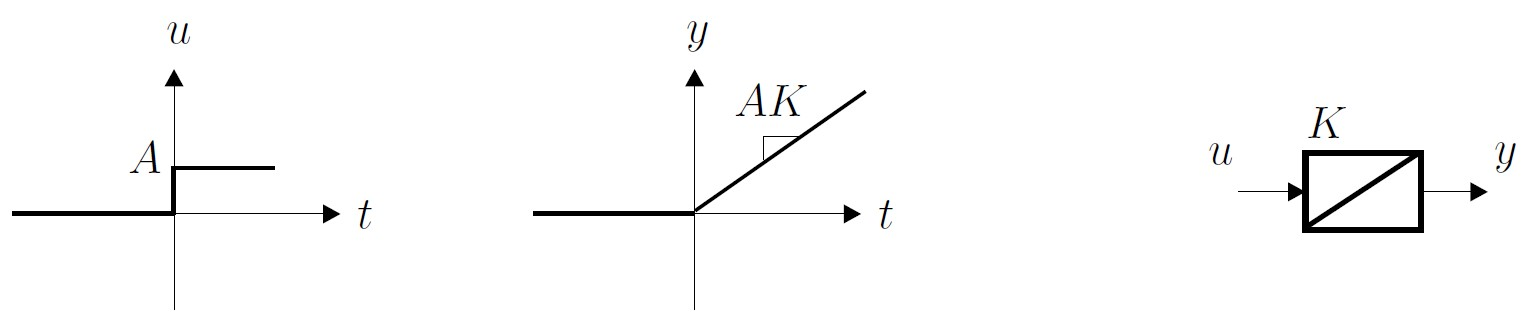
\includegraphics[width=0.9\columnwidth]{images/RegT1_grundglieder/i-glied} 


\subsection[PT1-Glied]{$\text{PT}_1$-Glied}

Ein Energiespeicher \textrightarrow\ System schwingt nicht

\begin{minipage}{0.48\columnwidth}
    $$ \boxed{ \text{DGL: } T \, \dot{y}(t) + y(t) = K \cdot u(t) }  $$
\end{minipage}
\hfill
\begin{minipage}{0.48\columnwidth}
    $$ \boxed{ y(t) = K \, A + (y_0 - K \, A) \cdot e^{- \frac{t}{T}} } $$
\end{minipage}


\begin{minipage}{0.5\columnwidth}
    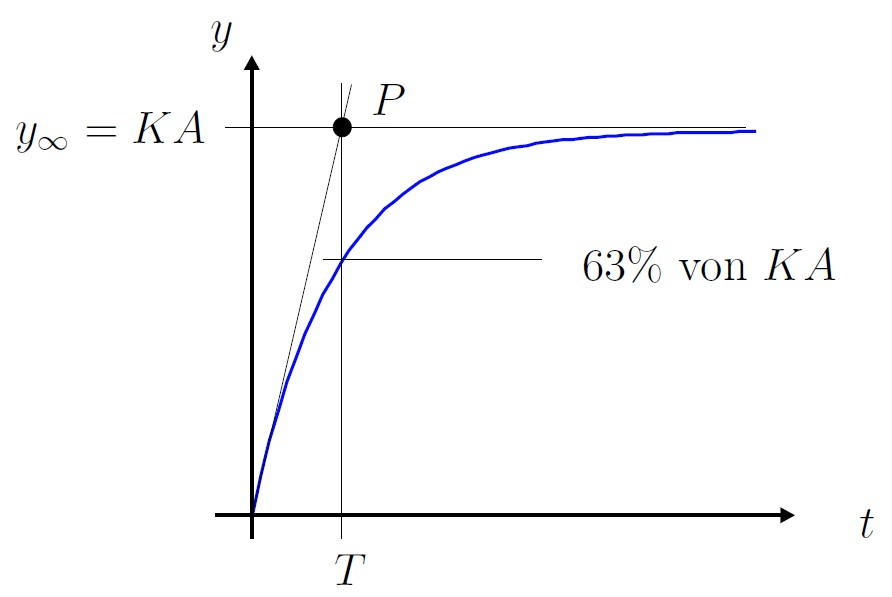
\includegraphics[width=\columnwidth]{images/RegT1_grundglieder/pt1-glied_kennlinie}
\end{minipage}
\hfill
\begin{minipage}{0.4\columnwidth}
    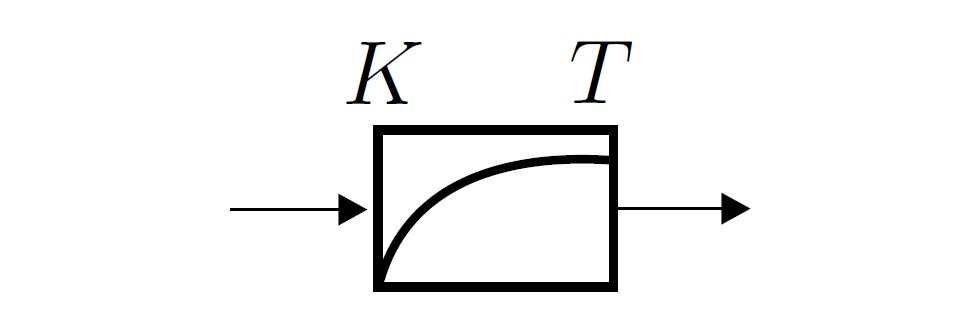
\includegraphics[width=0.8\columnwidth]{images/RegT1_grundglieder/symbol_PT1-glied}
\end{minipage}


\subsubsection{Modellierung einer $\text{PT}_1$ Regelstrecke}

\begin{itemize}
    \item Ausmessen der Sprungantwort $u(t) = A \cdot \varepsilon(t)$ \\
        \textrightarrow\ Die Sprungantwort entspricht dem Diagramm
    \item Parameter $K$ berechnen: $K = \frac{y_\infty}{A}$ 
    \item Parameter $T$ bestimmen: Tangente am Anfang durch Punkt $P$ \\
        oder: Zeit bis $y(T) = 0.63 \cdot K \, A$ erreicht ist \textrightarrow\ $T$ ablesen
\end{itemize}


\example{$\text{PT}_1$-Glied als Blockschaltbild}

\begin{minipage}{0.48\columnwidth}
    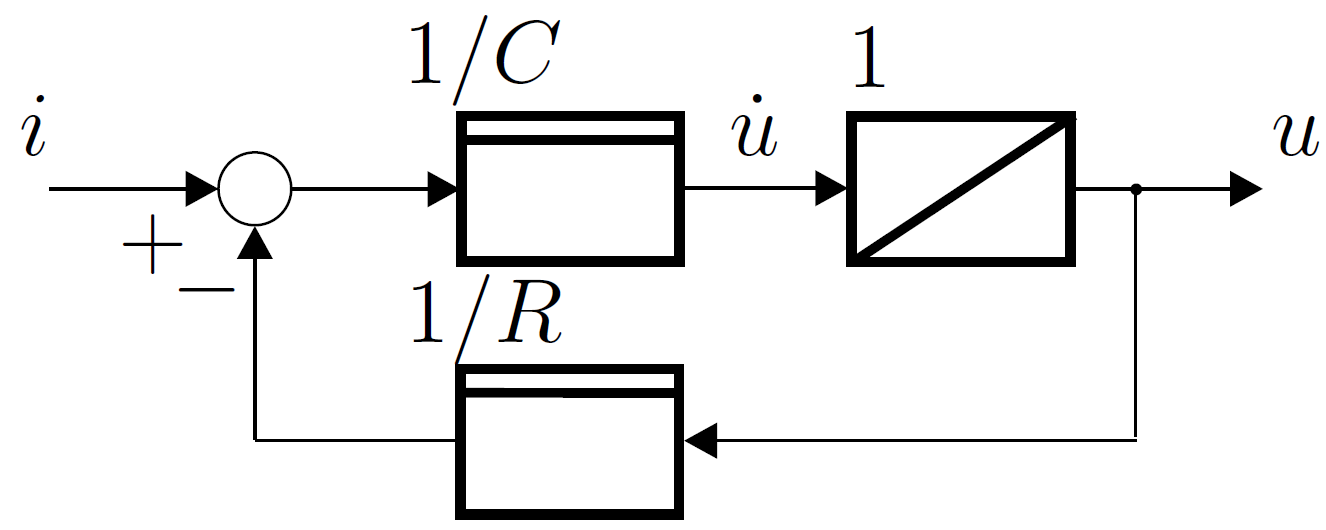
\includegraphics[width=\columnwidth]{images/RegT1_grundglieder/pT1_blockschaltbild}
\end{minipage}
\hfill
\begin{minipage}{0.48\columnwidth}
    $$ \boxed{ \text{Allg: } T \, \dot{y}(t) + y(t) = K \cdot u(t) }  $$
    $$ \boxed{ \text{Bsp: } RC \, \dot{u}(t) + u(t) = R \cdot i(t) }  $$
\end{minipage}

%\columnbreak


\subsection[PT2-Glied]{$\text{PT}_2$-Glied}

Zwei Energiespeicher \textrightarrow\ \textbf{System kann schwingen}

\vspace{-0.1cm}

\begin{minipage}{0.4\columnwidth}
    $$ \boxed{ \text{DGL: } T^2 \cdot  \ddot{y} + 2 \, \zeta \, T \cdot \dot{y} + y = K \cdot u } $$
\end{minipage}
\hfill
\begin{minipage}{0.58\columnwidth}
    $$ \boxed{ y(t) = K \: A \big[ 1 + e^{\sigma t} \big( - \cos(\omega t) + \frac{\sigma}{\omega} \sin(\omega t)  \big)  \big] }  $$
\end{minipage}


\begin{minipage}{0.55\columnwidth}
    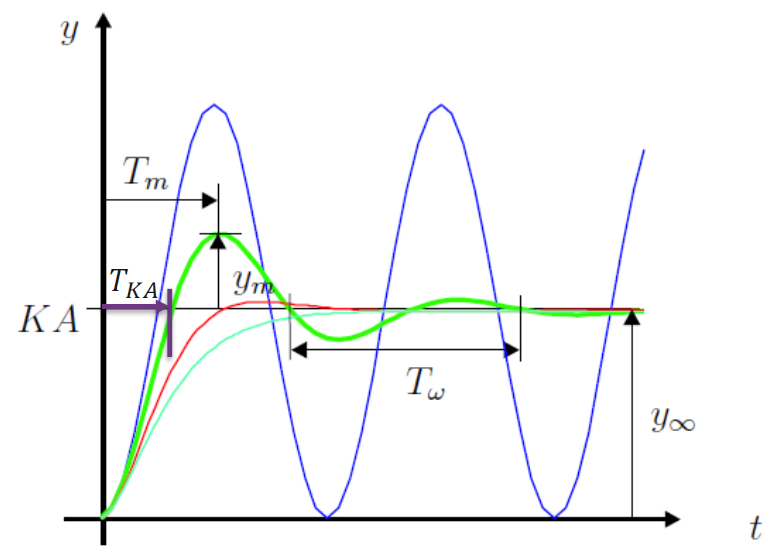
\includegraphics[width=\columnwidth]{images/RegT1_grundglieder/pT2_sprungantwort}
\end{minipage}
\hfill
\begin{minipage}{0.38\columnwidth}
    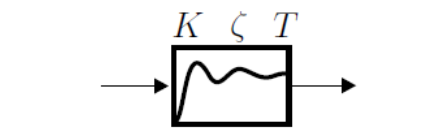
\includegraphics[width=0.75\columnwidth]{images/RegT1_grundglieder/pT2_symbol} 

    \begin{center}
        $ \omega = \omega_n \cdot \sqrt{1 - \zeta^2} $ \\
        $y_m = e^h \cdot y_{\infty}$ \\
    \end{center}
\end{minipage}


\begin{tabular}{c c c}
    $ K = \frac{y_{\infty}}{A}$                                                     & $ h = \ln \big( \frac{y_m}{y_{\infty}} \big)$                                 & $ \omega = \frac{2 \, \pi}{T_{\omega}} = \frac{\pi}{T_m} $ \\

    \rule{0pt}{10pt}$ \sigma = \frac{h \, \omega}{\pi} = - \omega_n \cdot \zeta$    & $ \omega_n = \sqrt{\omega^2 + \sigma^2} = - \frac{\sigma}{\zeta}$             & $ \zeta = - \frac{h}{\sqrt{h^2 + \pi^2}} $ \\

    \rule{0pt}{10pt}$T = \frac{1}{\omega_n}$                                        & $T_{KA} = T_M - \frac{1}{\omega} \arctan \big(  \frac{\omega}{\sigma} \big)$  & $y(T_{KA}) = K \: A$ \\
\end{tabular}

\vspace{0.2cm}
\textrightarrow\ $\zeta = \frac{1}{\sqrt{2}}$ entspricht 5 \% Überschwingen!


\subsection{D-Glied (Idealer Differenzierer)}

\vspace{-0.2cm}

$$ \boxed{  y(t) = K \cdot \frac{\diff u(t)}{\diff t} = K  \cdot \dot{u}(t) } $$

\begin{minipage}{0.25\columnwidth} 
    \begin{center}
        \myul{\textbf{ideal}}
    \end{center}

    \vspace{-0.1cm}

    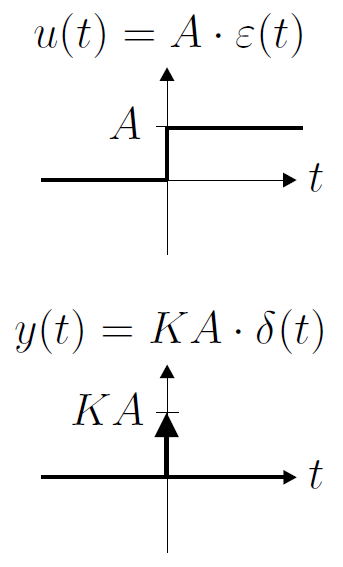
\includegraphics[width=0.65\columnwidth]{images/RegT1_grundglieder/D-glied_ideal}
\end{minipage}
\hfill
\begin{minipage}{0.25\columnwidth}
    \begin{center}
        \myul{\textbf{real}}
    \end{center}

    \vspace{-0.1cm}

    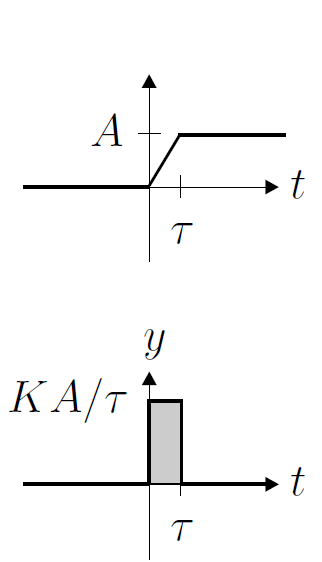
\includegraphics[width=0.6\columnwidth]{images/RegT1_grundglieder/D-glied_real}
\end{minipage}
\hfill
\begin{minipage}{0.25\columnwidth}
    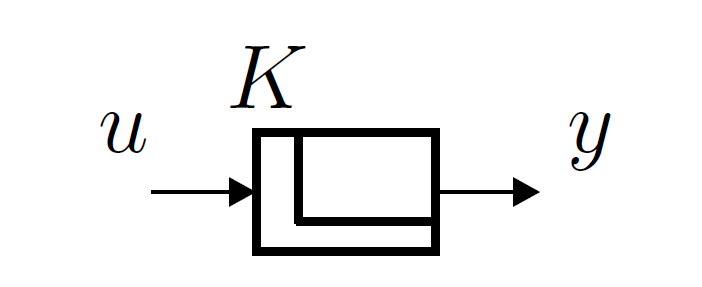
\includegraphics[width=0.9\columnwidth]{images/RegT1_grundglieder/D-glied_symbol}
\end{minipage}


\subsection[DT1-Glied (Realisierbarer Differenzierer)]{$\text{DT}_1$-Glied (Realisierbarer Differenzierer)}

\vspace{-0.1cm}

\begin{minipage}{0.48\columnwidth}  
    $$ \boxed{ w(t) = A \cdot (1 - e^{-\frac{t}{T}}) } $$
\end{minipage}
\hfill
\begin{minipage}{0.48\columnwidth}
    $$ \boxed{ y(t) = \frac{K \cdot A}{T} \,  e^{-\frac{t}{T}} } $$
\end{minipage}

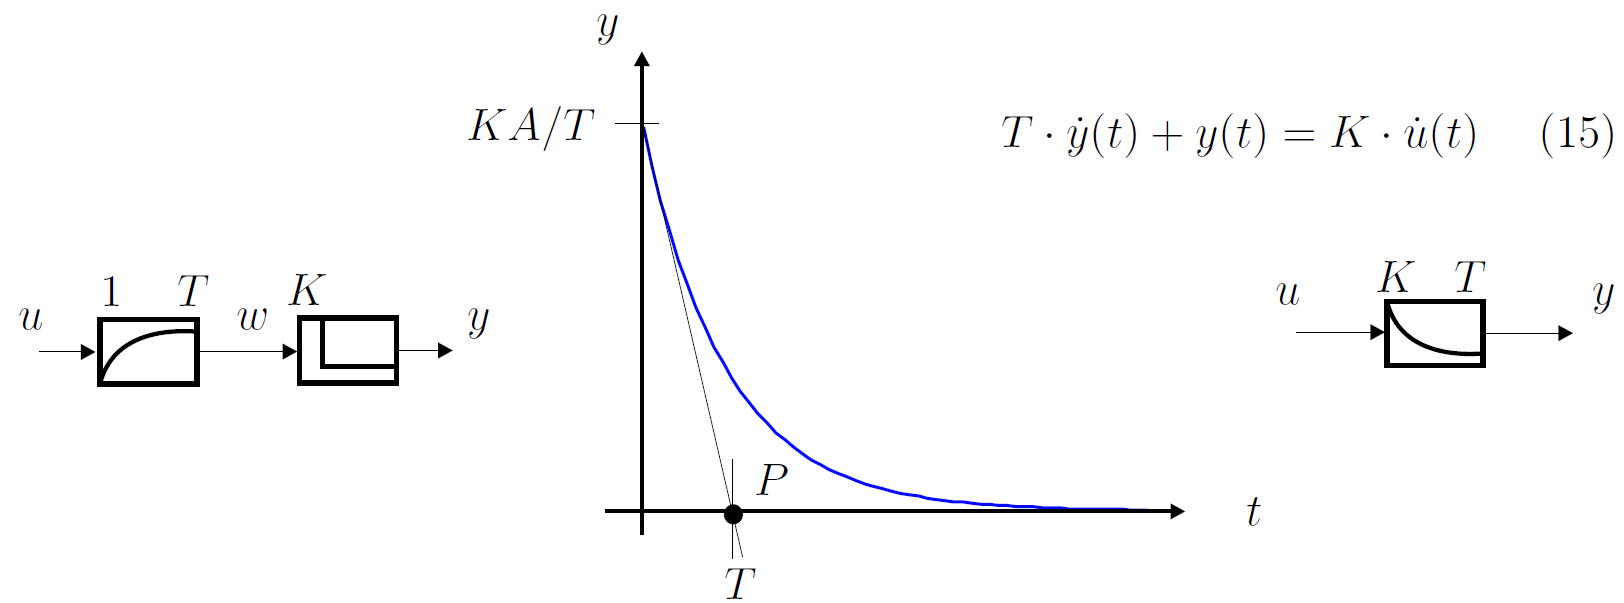
\includegraphics[width=\columnwidth]{images/RegT1_grundglieder/DT1-glied}


\example{Mögliche Realisierungen von $\text{DT}_1$-Gliedern}

\begin{minipage}[t]{0.48\columnwidth}
    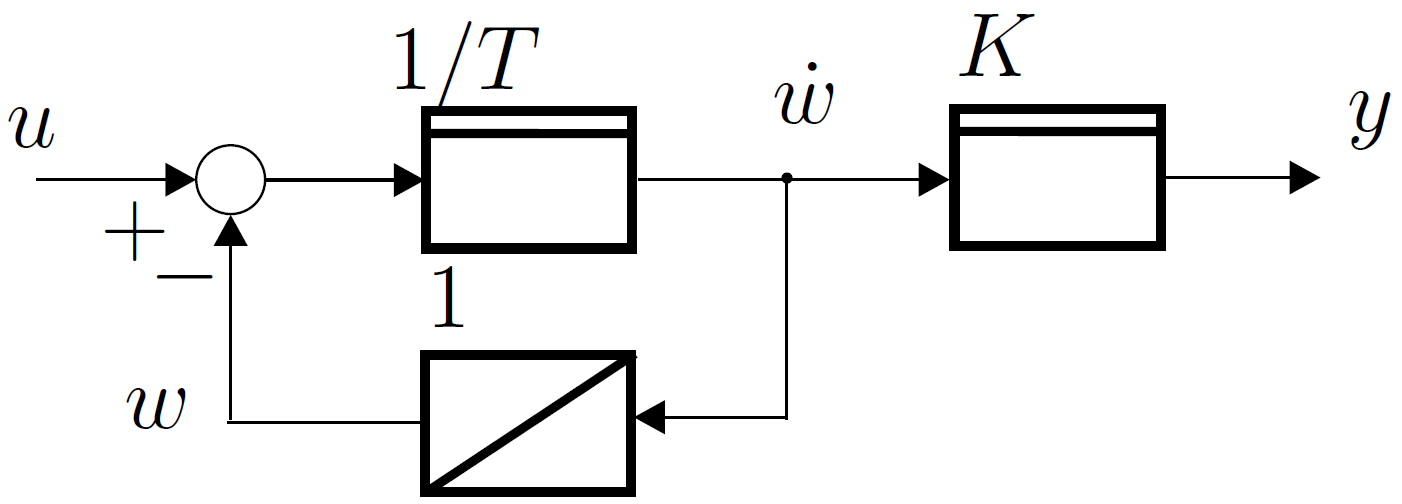
\includegraphics[width=\columnwidth, align=t]{images/RegT1_grundglieder/pT1_blockschaltbild_2}
\end{minipage}
\hfill
\begin{minipage}[t]{0.48\columnwidth}
    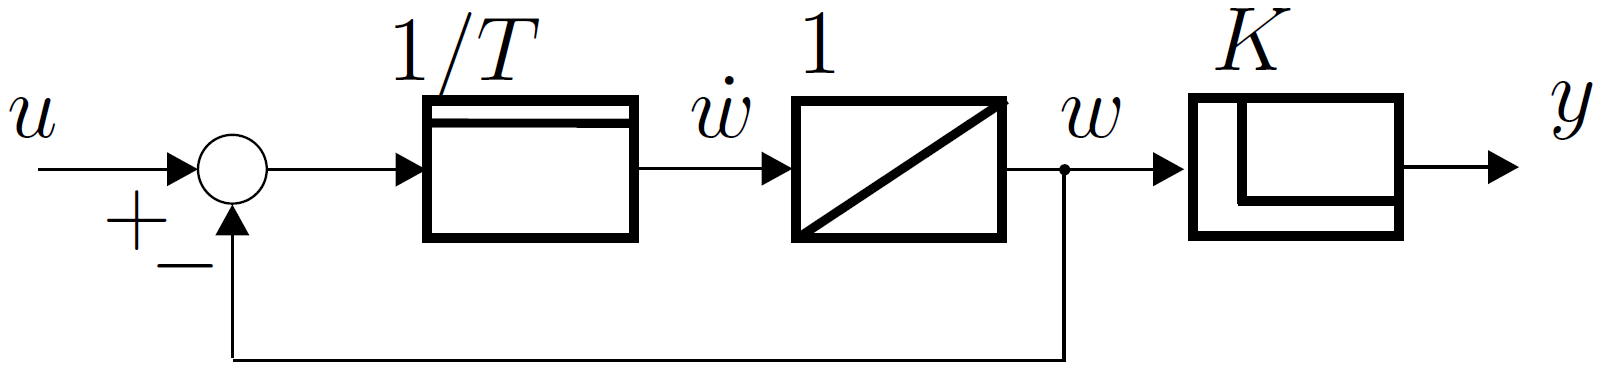
\includegraphics[width=\columnwidth, align=t]{images/RegT1_grundglieder/DT1-glied_blockschaltbild}
\end{minipage}



\subsection{Lead-Glied / Lag-Glied / Lead-Lag-Glied}

Lead-/ Lag-Glieder sind zwei Varianten von $\text{PDT}_1$-Gliedern. 

\begin{tabular}{ll}
    Lead:   & $K_P$ und $K_D$ haben \textbf{gleiches} Vorzeichen \\
    Lag:    & $K_P$ und $K_D$ haben \textbf{unterschiedliches} Vorzeichen \\
\end{tabular}

Lead- und Lag-Glieder können auch als Parallelschaltungen eines P- und eines $\text{PT}_1$-Glieds aufgefasst werden. 
Das Lead-Lag-Glied ist eine Serieschaltung aus Lead- und Lag-Glied.

\vspace{0.2cm}

\begin{minipage}[t]{0.45\columnwidth}
    \begin{center}
        \myul{\textbf{Lead-Glied}}
    \end{center}
    
    \vspace{-0.1cm}

    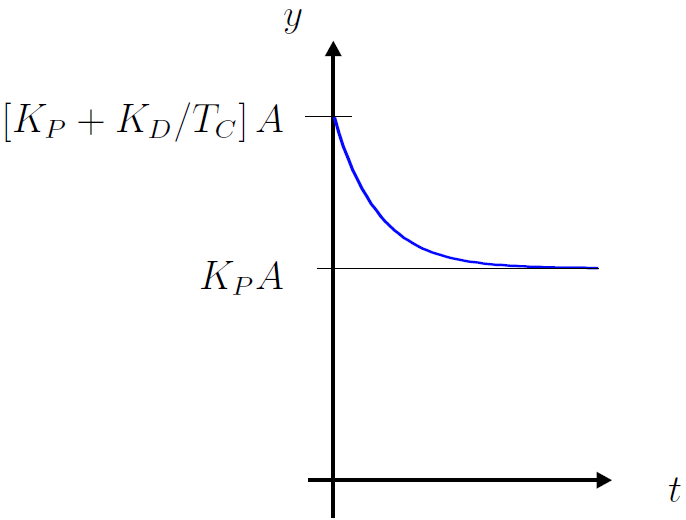
\includegraphics[width=0.9\columnwidth, align=t]{images/RegT1_grundglieder/lead-glied}
\end{minipage}
\hfill
\begin{minipage}[t]{0.45\columnwidth}
    \begin{center}
        \myul{\textbf{Lag-Glied}}
    \end{center}
    
    \vspace{-0.1cm}

    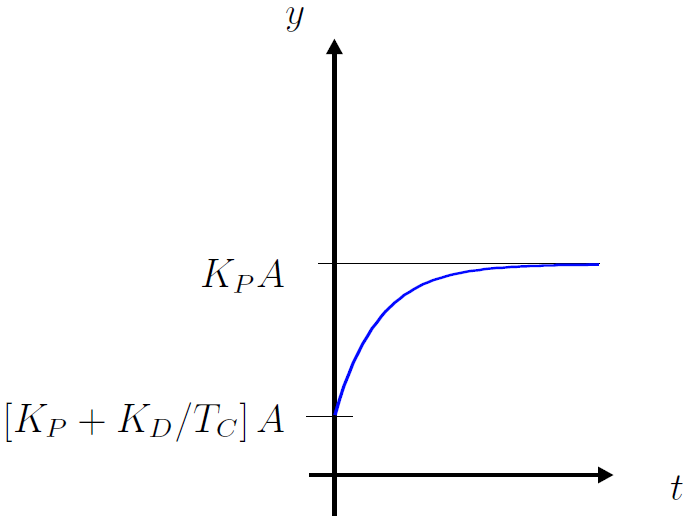
\includegraphics[width=0.9\columnwidth, align=t]{images/RegT1_grundglieder/lag-glied}
\end{minipage}

\section*{Prüfungscheck / Schnellreferenz}

\subsection*{Steuerbarkeit}
\[
Q_S=[B \;\; AB \;\; A^2B \;\; \dots \;\; A^{n-1}B]
\]

Vollständig steuerbar:
\[
\mathrm{rang}(Q_S)=n
\]

Steuerbar:
\[
\det(Q_S)\neq0
\]
(SISO-Fall)

\subsection*{Beobachtbarkeit}
\[
Q_B=
\begin{bmatrix}
C\\
CA\\
CA^2\\
\vdots\\
CA^{n-1}
\end{bmatrix}
\]

Vollständig beobachtbar:
\[
\mathrm{rang}(Q_B)=n
\]

\subsection*{Minimalität}
System minimal
\[
\Longleftrightarrow
\]
steuerbar \textbf{und} beobachtbar.

\subsection*{Zustandsrückführung}
\[
u=-Kx+r
\]

Geschlossener Kreis:
\[
\dot x=(A-BK)x+Br
\]

Pole:
\[
\lambda(A-BK)
\]

Polvorgabe nur möglich falls:
\[
\mathrm{rang}(Q_S)=n
\]

\subsection*{Beobachter}
\[
\dot{\hat x}=A\hat x+Bu+H(y-\hat y)
\]

\[
\hat y=C\hat x
\]

Beobachterpole:
\[
\lambda(A-HC)
\]

\subsection*{Transitionsmatrix}
\[
\Phi(t)=e^{At}
\]

\[
A=\dot{\Phi}(0)
\]

Diagonalform:
\[
e^{\Lambda t}
=
\mathrm{diag}
\left(
e^{\lambda_1 t},
\dots,
e^{\lambda_n t}
\right)
\]

\subsection*{Impulsantwort}
Kontinuierlich:
\[
g(t)=Ce^{At}B+D\delta(t)
\]

Diskret:
\[
g(k)=CA^{k-1}B
\qquad (k\ge 1)
\]

\subsection*{Stabilität}
Zeitkontinuierlich:
\[
\mathrm{Re}(\lambda_i)<0
\]

Zeitdiskret:
\[
|\lambda_i|<1
\]

\subsection*{Trajektorienbilder}
\begin{itemize}
\item $\lambda<0$: Ursprung attraktiv
\item $\lambda>0$: Ursprung abstossend
\item $\lambda=\pm j\omega$: Kreisbewegung
\item Jordanblock: Scherbewegung
\end{itemize}

\subsection*{Prüfungsklassiker}
\begin{itemize}
\item UTF $\leftrightarrow$ ZRD
\item Blockdiagramm $\rightarrow$ ZRD
\item Steuerbarkeit / Beobachtbarkeit
\item Polvorgabe
\item Transitionsmatrix
\item Impulsantwort / Faltung
\item ZOH-Diskretisierung
\item Wurzelortskurve
\end{itemize}

\subsection*{Sofortwissen}

\[
G(s)=C(sI-A)^{-1}B+D
\]

\[
\tilde A=PAP^{-1}
\]

\[
\tilde B=PB
\]

\[
\tilde C=CP^{-1}
\]

Eigenwerte bleiben bei der Ähnlichkeitstransformation unverändert.
    \end{layout}

    \include{sections/100_anhang_regt2_tabellen.tex}
\end{document}
